% tnf_paper_v2.tex --- v2, rebuilt 2026-08-11.
%
% v1 (tnf_paper.tex, 4273 lines) is UNCHANGED and remains the record of what was
% claimed before the block-axis headline was refuted. This file is a rebuild, not
% an edit: the spine is the three parameters of a shared block scale (base,
% alignment, width), the phi-grid domination claim is withdrawn where it was
% made, and the fixed-field-versus-tapered material is moved to a companion
% instrument paper rather than left in a chapter with no argument to serve.
%
% Measured on XC7A200T through the open flow. Every frequency in this paper is an
% unconstrained post-route critical-path estimate and is labelled as one.

\documentclass[11pt]{article}

\usepackage[utf8]{inputenc}
\usepackage[T1]{fontenc}
\usepackage{hyperref}
\usepackage{graphicx}
\usepackage{booktabs}
\usepackage{amsmath}
\usepackage{amssymb}
\usepackage{url}
\usepackage{geometry}
\usepackage{tabularx}
\usepackage{array}
\usepackage{enumitem}
\usepackage{amsthm}
\newtheorem{theorem}{Theorem}
\newtheorem{proposition}[theorem]{Proposition}
\newtheorem{corollary}{Corollary}
\theoremstyle{definition}
\newtheorem{definition}{Definition}

\geometry{a4paper, margin=1in}

\hypersetup{
  colorlinks=true,
  linkcolor=blue,
  urlcolor=blue,
  citecolor=blue
}

% v2: a little emergency stretch removes the marginal overfull boxes the
% rebuilt paragraphs introduce without changing any wording.
\setlength{\emergencystretch}{1em}
% v2. The title names the object this paper takes apart --- the shared block
% scale --- and the three parameters it decomposes into. v1 named a format (TNF)
% and a pair; both halves of that subtitle are damaged by our own measurements.
% The v1 comment is kept below for the record.
% ---- v1 comment ----
% The title names the category and the design point rather than an internal
% codename. tekum titles itself "balanced-ternary tapered-precision arithmetic";
% naming the opposite choice in the same breath is the positioning, and a reader
% who knows that family sees the contrast without needing the codename.
% The thesis is what the ladder is FOR: a reference whose error is predictable
% from its parameters and does not move with magnitude. Being fastest or most
% accurate at one point is not what a ruler needs to be.
\title{%
  \fontsize{30}{34}\selectfont\bfseries Base, Alignment, Width\\[10pt]
  \normalfont\large A shared block scale is three parameters and not one:
  the base is closed by a cost theorem under a stated alphabet, the field
  carries four bits that no weight tensor at a deployed block size uses, and
  the alignment --- fixed by every specification and tuned by none --- is worth
  $2.78$ and $0.51$ perplexity on two models, at one constant and at $4.125$
  bits per weight; the datapath that reads it has no multiplier anywhere and
  accumulates exactly in $32$ bits}

\author{Dmitrii Vasilev\\
  \small ORCID 0009-0008-4294-6159 \\
  \small \texttt{admin@t27.ai}}
\date{11 August 2026}

% Floats were sitting flush against the text above them. Set the three
% float separations once rather than nudging tables individually.
\setlength{\textfloatsep}{20pt plus 4pt minus 4pt}
\setlength{\intextsep}{20pt plus 4pt minus 4pt}
\setlength{\floatsep}{20pt plus 4pt minus 4pt}
\setlength{\abovecaptionskip}{8pt}
\setlength{\belowcaptionskip}{4pt}

\begin{document}
\maketitle

\begin{abstract}
A deployed four-bit tensor is a block of elements and a scale they share. The
element has been designed and redesigned; the scale is one number per
thirty-two weights and is copied out of the specification. It is not one
parameter but three --- the \textbf{base} $g$ of its ladder, the
\textbf{alignment} $c$ that decides where the ladder's window sits under the
element's maximum, and the \textbf{field width} $b$ that stores it. This paper
takes the three apart. One is closed by a proof, one is over-provisioned by
four bits and was observed before us, and the third is free, is tuned by
nobody, and is worth more than the other two together.

\textbf{The base is closed, under a stated alphabet.} Applying $r^{k}$ without
a multiplier is a sparsest-multiple problem, not a sparsity count on the
minimal polynomial: $r = 1.290648801$ has minimal polynomial
$x^4-x^3+x^2-x-1$ and costs three adders read that way, yet $r^{5} = 2r+1$
costs one. Proved: the adder cost $A(r)$ is zero exactly when $r$ is a rational
power of two, and $A(r)=1$ exactly when some monic annihilator of $r$ has
non-leading weight two. Restricting the annihilator's coefficients to
$\{0,\pm1\}$, every one-adder ratio in $(1,2)$ is at most $\varphi$, equality
only for $r^{2}=r+1$ --- so under that alphabet nothing lies between the shift
and $\varphi$ at one adder, proved where a previous version enumerated. The
restriction is load-bearing and we state it rather than bury it: a coefficient
of $2$ is a shift, free on the same cost model, and admitting it puts eight
ratios into $(\varphi,2)$ at degree at most six, the smallest $r = 1.695621$
with $r^{3}=r^{2}+2$. Separately, $\sqrt{2}$ and $2^{1/4}$ are rational powers
of two and so cost no adder at all under this model, making them finer than
$\varphi$ and cheaper --- which Miyashita et al.\ used in
2016~\cite{miyashita} and Vogel et al.~\cite{vogel} generalised in 2018.

\textbf{We withdraw our own base claim.} A previous version reported a
$\varphi^{k}$ scale grid at four bits strictly dominating MXFP4 on two models.
The two arms differed in alignment as well as in base. Reparameterised so that
each base is measured at its \emph{own} best alignment --- 40 windows of
$2048$ tokens of wikitext-2, block of $32$, E2M1 elements, weight-only,
\texttt{fp32} forward, \texttt{lm\_head} excluded, both optima selected on that
same evaluation set --- $2^{k}$ wins on both models: $20.6950$ against
$21.3112$ on SmolLM2-135M (\texttt{fp32} baseline $14.4874$) and $14.5532$
against $14.7850$ on Qwen2.5-0.5B (baseline $12.2277$). It is not a knife edge:
$2^{k}$ beats $\varphi$'s best at \emph{every} alignment in $u\in[0.15,0.35]$
on SmolLM2 and $u\in[0.10,0.30]$ on Qwen, and the ranking survives all three
element tie rules. Equal bits is not equal span: sixteen levels of $\varphi$
cover $10.41$ binades against $2^{k}$'s $15.00$.

\textbf{The alignment is free, and it is the result.} The MX
specification~\cite{ocpmx} fixes the alignment constant at $c = 4$ for base two
--- nominally $41.5\%$ of the window clamped --- and that setting is the first
point on the rising side of a basin. Moving that one constant to
$c = \texttt{max\_norm}/2^{0.7} = 3.6934$, on a plain power-of-two ladder, with
no new arithmetic and at $4.125$ bits per weight: $23.5224 \to 20.7384$ on
SmolLM2 and $15.0638 \to 14.5532$ on Qwen. One constant, both models, no
per-model tuning; each model's own argmin buys a further $0.04$ and $0.00$. The
same retuning is worth $0.04$ to a $\varphi$ ladder, whose default alignment
already sat within $0.04$ of its optimum --- so alignment accounts for the
whole of the apparent $\varphi$ advantage and more, and with both bases aligned
the base axis reverses sign.

\textbf{The field is over-provisioned, and saying so is not ours.} A field of
$b_{\min}(W,K) = \lceil \log_{2} S(W,K)\rceil$ exponent bits, plus a per-tensor
anchor exponent, is sufficient and returns a \emph{bitwise identical} tensor to
E8M0. Measured on five checkpoints at $K=32$ --- SmolLM2-135M, Qwen2.5-0.5B,
Pythia-160M, OPT-125M, GPT-2 --- $b_{\min} = 3,4,3,4,4$, and a four-bit field
clamps zero of $20{,}462{,}464$ blocks. That a four-bit exponent suffices was
stated first by Chhugani et al.~\cite{chhugani}; our contribution is the
formula, the proof of bitwise identity, and the boundary --- four bits fails at
$K \leq 2$ on all five checkpoints and at $K = 4$ on GPT-2, and activations
need five.

\textbf{The datapath.} The weight alphabet $\{-\varphi,0,+\varphi\}$ closes
$\mathbb{Z}[\varphi]$ under weight application and accumulation, so a layer's
linear path is exact; machine-checked in Coq, with $\varphi^{2}=\varphi+1$ and
the exactness of the whole dot product both discharged by \texttt{Qed} and no
\texttt{Admitted} in the file (\texttt{golden\_alphabet/GoldenAlphabet.v};
the artefact is named because a sibling repository carries an
\emph{admitted} statement of the same identity). Measured over all $210$
SmolLM2 tensors and $42{,}024{,}960$ accumulations, that path needs $19$ bits
on real activations and $21$ in an attained worst case over all \texttt{int8}
vectors, so a $32$-bit integer pair carries it with eleven bits spare. The
block scale is what makes that width possible: on a single global
$\varphi^{k}$ grid of span $43$ one term alone needs $36$ bits. On an XC7A200T
a ternary neuron costs $28$ LUT per weight and \emph{no DSP at any fan-in}.

Every claim this campaign withdrew --- the block-axis headline above among them
--- is retracted where it was made and enumerated in one ledger
(Section~\ref{sec:selfcheck}). Every frequency in this paper is an
unconstrained post-route critical-path estimate and is labelled as one at the
point of use.
\end{abstract}


\section{What this paper argues}
\label{sec:roadmap}

The results below were found in the order a measurement campaign finds things.
They compose into one argument, and the argument is easier to follow stated
first.

\paragraph{The object, and why it has been overlooked.} A four-bit tensor as
deployed is two things: an element code, and a scale shared by a short block of
elements. Almost all recent work varies the first, or varies a rotation applied
before it. The scale is one number per $K$ weights, its cost is amortised
$K$-fold, and it is copied from whichever specification the element came from.
Copied, it looks like one parameter. It is three. Writing the rule that every
microscaling format uses,
\begin{equation}
\label{eq:scalerule}
  s \;=\; g^{\,\lfloor \log_{g}(a_{\max}/c) \rfloor},
  \qquad\text{so that}\qquad a_{\max}/s \in [\,c,\; c\,g\,),
\end{equation}
the free choices are the \textbf{base} $g$ of the ladder, the
\textbf{alignment} $c$ that places the window $[c, cg)$ relative to the element
format's largest magnitude, and the \textbf{width} $b$ of the field that stores
the exponent. Sections~\ref{sec:hierarchy}, \ref{sec:alignment}
and~\ref{sec:scalewidth} take those three in turn, and the shape of the answer
is the shape of the paper: the base admits an unconditional answer, the width
admits one that is not ours, and the alignment --- the only one no
specification names --- is where the value is.

\paragraph{The opening move is a correction to our own optimality result.}
A previous version of this paper closed its format-design chapter with a
corollary, \emph{three inputs determine the format}: name the fabric, the
required range, and which side of the fixed-field/taper dichotomy the workload
sits on, and the layout follows. That corollary is incomplete, and
Section~\ref{sec:threeparams} says how. Its three inputs fix the element and
the split between exponent and mantissa. None of them fixes where a shared
scale's window sits under the element's maximum, because in a per-tensor format
there is no such parameter to fix --- it appears only when a scale is shared.
There is a fourth input, it is free, and on the measurements below it moves
perplexity by $2.78$ at a single constant where the other three move it by
fractions of that. We
prefer to open on the incompleteness rather than on the withdrawal, because the
incompleteness is what makes the withdrawal predictable in hindsight.

\subsection*{The base: closed, and closed against us}

\paragraph{What a multiply-free scale costs, exactly.} A scale ladder is
applied by repeated multiplication by $r$, and the question is how many adders
that costs. Section~\ref{sec:hierarchy} shows the previously used answer is the
wrong invariant. Cost is not the sparsity of $r$'s minimal polynomial; it is
the sparsest multiple of it. The witness is $r = 1.290648801$, whose minimal
polynomial $x^{4}-x^{3}+x^{2}-x-1$ has three non-leading terms and therefore
three adders on the old reading, while $r^{5} = 2r+1$ applies it with one. The
correct statements are two, and both are proved: the adder cost $A(r)$ is zero
exactly when $r$ is a rational power of two, and $A(r)=1$ exactly when some
monic annihilator of $r$ has non-leading weight two.

\paragraph{Two consequences, one of which is an upgrade and one a kill.} The
upgrade: under coefficients in $\{0,\pm1\}$, every one-adder ratio in $(1,2)$
is at most $\varphi$, with equality only for $r^{2}=r+1$. The proof is two
lines --- for $r>\varphi$ and $m>k\geq 1$, $r^{m}-r^{k}-1 \geq r^{k}(r-1)-1
\geq r(r-1)-1 > 0$ --- and it replaces a claim the previous version supported
by enumerating degrees. \emph{Nothing lies between the shift and $\varphi$ at
one adder} is now a theorem rather than a search that had not yet failed. The
kill: rational powers of two are free, so $\sqrt{2}$ and $2^{1/4}$ are strictly
finer than $\varphi$ and strictly cheaper than it. The previous version's
sentence \emph{among multiply-free grids, $\varphi^{k}$ is the finest available
at four bits} is therefore false, and it was false before any perplexity was
measured. Miyashita et al.~\cite{miyashita} quantised to base $\sqrt{2}$ and
base $2^{1/4}$ in 2016, and Vogel et al.~\cite{vogel} built multiplierless
FPGA inference at an arbitrary logarithmic base in 2018. On the base axis of a
scale ladder we are late, and the correct posture is to say so.

\paragraph{And the measurement agrees with the algebra.} Section~\ref{sec:confound}
retracts the claim that a $\varphi^{k}$ grid at four bits dominates MXFP4. The
comparison that produced it gave $\varphi$ its natural no-clamp alignment and
gave $2^{k}$ the specification's, so the arms differed in two parameters and
the difference was attributed to one. Reparameterised base-independently by
the nominal clamp fraction $u$, with $c = \texttt{max\_norm}/g^{\,1-u}$ so that
$u=0$ is no-clamp for either base and $u = 0.41504$ is exactly the MX
specification, and measured at each base's own best alignment, $2^{k}$ wins on
both models --- $20.6950$ against $21.3112$ on SmolLM2 and $14.5532$ against
$14.7850$ on Qwen --- and wins at every $u$ in $[0.15, 0.35]$ and
$[0.10, 0.30]$ respectively rather than at a single point. A second and
independent objection applies to the same claim: on Qwen the reported margin
was $14.9447 - 14.8512 = 0.0935$, and switching the element tie-break rule
alone moves the $2^{k}$ arm of that comparison by $0.0932$ --- the same size as
the entire margin, to three decimal places; on SmolLM2 the same switch is worth
$0.129$. The number was uninterpretable before alignment was ever considered.
At the corrected comparison the nuisance decides nothing: across the three
rules the spread is $0.0455$ on SmolLM2 and $0.0287$ on Qwen at each base's own
best alignment, against margins of $0.6162$ and $0.2318$, and $\varphi$ minus
$2^{k}$ stays positive in all six cells ($+0.6162$, $+0.5838$, $+0.3706$;
$+0.2318$, $+0.2030$, $+0.2099$). One anomaly in that table is unresolved and
we record it rather than smooth it: under ties-to-away the $\varphi$ arm moves
$0.2001$ on SmolLM2 although the same run finds no normalised weight exactly on
an E2M1 midpoint under a $\varphi$ scale. A rule that can act only on exact
midpoints should not move a configuration that has none, and until that is
explained the $\varphi$ arm's ties-to-away column is not to be quoted.

\paragraph{Which rung, then, and reported as measured.} The hierarchy the cost
theorem closes is still a hierarchy, and Section~\ref{sec:fivefamilies} asks which
of its rungs to spend a weight budget on. Measured on five model families ---
SmolLM2, Qwen, Pythia, OPT and GPT-2, weight-only --- three bits wants the plain
shift and five bits wants the plastic number, on all five. Four bits does not
settle: across models it returns $\varphi$, $\varphi$ and the supergolden ratio.
We report the four-bit rung as a
per-model measurement and not as a prediction, and we withdraw the closed form
that had predicted it, whose validation was circular and whose stated regularity
fails in $20$ of the $25$ cells it was fitted on.

\paragraph{Why a $\varphi$ ladder loses even where it is finer.} Its step is
finer --- $\log_{2}\varphi = 0.694$ binades against $1.000$ --- and at equal
field width its span is shorter, sixteen levels covering $10.41$ binades
against $15.00$. Equal bits is not equal span, and a scale field that runs out
of range costs more than a scale field that steps coarsely, which is the
asymmetry Section~\ref{sec:widthrule} proves and Section~\ref{sec:alignment}
measures.

\subsection*{The alignment: free, untuned, and the largest term}

\paragraph{The result.} Section~\ref{sec:alignment} sweeps $u$ on a plain
power-of-two ladder with the element format untouched. The response is a basin,
not a plateau with a cliff at the end of it. On SmolLM2 it falls from $22.7120$
at $u=0$ to a floor of $20.6950$ --- $22.1478$, $21.3716$, $21.1493$,
$20.9775$, $21.0100$, $20.7384$, $20.6950$ at $u=0.05$ through $0.35$ in steps
of $0.05$ --- a decline of $2.02$, with one $0.03$ reversal at $u=0.25$ and a
floor flat enough ($0.04$) that the argmin is not resolved between $u=0.30$ and
$u=0.35$. Past the floor it rises steeply: $23.5224$ at the specification's
$u = 0.41504$, $25.6081$ at $0.45$, $27.7307$ at $0.50$, $31.8413$ at $0.55$.
The deployed constant is the first sampled point on the rising side. Moving it
to $u=0.30$ and nothing else takes SmolLM2 from $23.5224$ to $20.7384$ and Qwen
from $15.0638$ to $14.5532$, at $4.125$ bits per weight --- below MXFP4's
$4.250$, and with the same arithmetic, the same element codebook and the same
block size. The change is one constant in the scale rule, and it is the same
constant on both models.

\paragraph{The instrument, once, for every block number in this paper.} All of
them come from one harness, written from scratch after two earlier ones were
found to have flattered $\varphi$ in different ways, and it aborts before
printing anything if a gate fails: the SmolLM2 run logs $38$ global assertions
in eight groups and $44$ per-model assertions in five. The element rounder is
checked against a brute-force scalar loop on $40{,}037$ probes under each of
the three tie rules, and the whole block pipeline --- \texttt{amax}, the
geometric scale, the field clamp, the sign, the reconstruction --- against a
third implementation in pure Python that shares no code with it and locates the
exponent by repeated multiplication rather than by a logarithm. The
\texttt{fp32} baselines it reproduces are $14.4874$ and $12.2277$; it
reproduces the specification-faithful MXFP4 figures $23.5224$ and $15.0638$ as
a gate; and it returns $21.3547$ for the $\varphi$ configuration the previous
version published as $21.3545$ --- so the retraction below is a change of
comparison and not a change of measurement. One caveat belongs with $u$ itself:
it is the clamp fraction of the window under a log-uniform model of the block
maximum, so it is nominal rather than measured. At $u = 0.41504$ the fractions
that actually clamp are $46.57\%$ on SmolLM2 and $40.18\%$ on Qwen, which
bracket it.

\paragraph{Why it is a basin with one steep wall.} The mechanism is the
element, not the field. Raising $c$ slides the window $[c,cg)$ up under
\texttt{max\_norm} $=6$, so a rising fraction of block maxima --- the largest
weight in each block, the one the scale was chosen to represent --- saturate to
the top code: $16.67\%$ at $u=0.15$, $39.62\%$ at $u=0.35$, $46.57\%$ at the
specification's $u=0.41504$, $60.11\%$ at $u=0.55$ on SmolLM2. Lowering $c$
instead leaves element codes unused above the block maximum, which costs
resolution on every weight rather than gross error on the largest. The two
costs are asymmetric in the same direction that Section~\ref{sec:widthrule}
proves for a range field --- gradual where the resource is wasted, abrupt where
it runs out --- and this sweep is the first instrument this paper has put on
that asymmetry. That the effect is alignment and not width is measured, not
assumed: the four-bit scale field clipped zero blocks in every cell of the
sweep, on both models and at both bases.

\paragraph{What this does and does not say about MXFP4.} It is not a new
format. The element stays E2M1, the field stays four bits wide inside E8M0's
eight, the block stays thirty-two, and only the constant that aligns the shared
exponent moves. Read as a contribution it belongs to the microscaling family
rather than against it, and it is available to anyone shipping MX today at the
cost of an off-by-one in an exponent computation.

\subsection*{The width: over-provisioned, and the observation is not ours}

\paragraph{Prior art first.} Chhugani et al.~\cite{chhugani} state, on
Llama-3.1-8B-Instruct and Qwen3-8B, that a four-bit exponent suffices for
MXFP4's shared scale, and explicitly propose truncating E8. QLoRA's double
quantisation~\cite{qlora} narrows a second-level scale for the same reason;
NVFP4~\cite{nvfp4} already pairs a per-tensor anchor with a narrow per-block
E4M3; and Shared Microexponents~\cite{msfp} makes the scale hierarchy itself
the design object. Section~\ref{sec:scalewidth} contributes the formula, not
the observation.

\paragraph{The formula, and what it buys.} $b_{\min}(W,K) = \lceil \log_{2}
S(W,K) \rceil$ bits, where $S$ is the span of the block-exponent histogram, is
\emph{sufficient} and returns a tensor bitwise identical to E8M0 --- not
approximately equal, identical --- so the four freed bits are free in the
strict sense. Necessity holds only in the worst case, and a counterexample is
constructed. The span behaves: $R < S < R+2$ on all $3{,}780$ tensor-$K$ pairs
measured, with no exceptions. At $K=32$ on five checkpoints $b_{\min}$ is
$3,4,3,4,4$, and a four-bit field clamps zero of $20{,}462{,}464$ blocks.

\paragraph{And where the constant breaks.} Four bits is not a law. Swept over
$K$ from $1$ to $256$, it holds for all five checkpoints at $K \geq 8$ and
fails at $K \leq 2$ on every one of them and at $K=4$ on GPT-2. Activations
break it outright: OPT needs five bits, with $12$ of $72$ layers over four and
a worst case of $30$ binades at \texttt{decoder.layers.7.fc2}, and the
mechanism is a downward tail --- post-ReLU near-zero blocks dragging $e_{\min}$
down some twenty-eight binades. Activation spans are sample-dependent and were
still growing when we stopped sampling. \emph{E8M0 is over-provisioned}
survives, because five is still less than eight; \emph{four bits} does not
survive contact with activations, and is stated for weights only.

\subsection*{The datapath this scale sits in}

\paragraph{An alphabet and an accumulator width close a ternary node.} A
ternary node has three sites that could carry a number format
(Section~\ref{sec:pair}): the weight is a code and multiplying by it is a
sign-select, the sample arrives ADC-native, and only the accumulator carries a
range that must be spent. The previous version answered the third with a float
ladder. Our own measurement says it wants a width instead.
Section~\ref{sec:closure} shows that removing a multiplier --- as against
cheapening one --- requires the weight lattice to be closed under weight
application, which $\mathbb{Z}[\varphi]$ is because $\varphi^{2}=\varphi+1$: a
weight application is the Fibonacci step $(a,b)\mapsto(b,a+b)$, accumulation is
componentwise, and the linear path is exact. That is machine-checked in Coq
with no admitted lemmas.

\paragraph{The width condition, corrected.} We published an accumulator width
\[
  W \;=\; \bigl\lceil \log_{2}\bigl(n\,A\,\max(F_S,1)\bigr) \bigr\rceil + 1 ,
\]
and it is sufficient and \emph{not} necessary. The reason is structural rather
than empirical:
componentwise two's-complement addition, the Fibonacci step and integer scaling
are all $\mathbb{Z}$-linear, and reduction modulo $2^{W}$ is a ring
homomorphism, so a $W$-bit datapath returns the exact result modulo $2^{W}$ and
intermediate overflow self-cancels. Bit-accurate simulation agrees: $12$ of
$12$ configurations exact below the bound, six of them with genuine
intermediate overflow. Measured over all $210$ SmolLM2 tensors and
$42{,}024{,}960$ accumulations, the final pair needs $19$ bits on real
activations and $21$ in a worst case attained over all \texttt{int8} vectors.
A $32$-bit accumulator therefore carries the path with eleven bits spare, good
to $72{,}572$ terms; a $16$-bit one fails at fan-in $512$, wrapping $669$ of
$42.0$ million, while remaining correct at the fan-ins of $8$, $16$ and $32$
that the node designs actually use.

\paragraph{And here the two halves of the paper meet.} The block scale is not
only an accuracy device: it is the enabling condition for the $32$-bit
accumulator. On a single global $\varphi^{k}$ grid, whose exponent span is
$43$, one term alone requires $127\,F_{43}$ and therefore $36$ bits. Sharing a
scale across a short block is what keeps the exact path inside a machine word.
That sentence is the join between the scale chapter and the datapath chapter,
and it did not exist in the previous version.

\paragraph{What exactness is worth, measured rather than asserted.}
Section~\ref{sec:exactbuys} prices it, because the theorem invites over-reading.
Summation order moves perplexity by $6.75\times10^{-6}$ on SmolLM2 and
$3.10\times10^{-5}$ on Qwen; exact accumulation against \texttt{fp32} differs
by $+8.4\times10^{-7}$ and $-1.05\times10^{-5}$, with the sign flipping between
the two models; and one, two, four and eight threads give bitwise identical
perplexity. Exactness removes \emph{scatter}, not \emph{error}, and
\texttt{fp32} is unbiased around the exact result. It begins to pay where the
accumulator narrows: relative order-scatter is $5.2\times10^{-7}$ at
\texttt{fp32}'s 24 significand bits, $4.4\times10^{-3}$ at \texttt{fp16}'s
eleven and $3.5\times10^{-2}$ at \texttt{bf16}'s eight. That is the regime in
which an exact integer accumulator earns its keep, and it is a narrower claim
than \emph{exact is better}.

\subsection*{The element half of the block axis is the competition's}

Section~\ref{sec:blockbound} reports where none of this wins. On a short block
with a shared scale, the codebook minimising squared error is not the one
minimising perplexity, and the gap between the best achievable eight-level
codebook and the deployed one is under one percent --- a margin that is itself
a property of where each codebook's top level sits inside its binade, so it is
requoted with every top normalised to $1$ and the phase held at zero. Two
further searches were run against that gap after the bound's original argument
was found to be wrong: a codebook fitted to the model's logits and one fitted
to its weight statistics. The first inverts its ranking out of sample; the
second keeps its sign and loses its magnitude, to a pooled out-of-sample effect
of $-0.16\%$ with $t = -0.22$ and a $95\%$ interval of $[-1.56\%, +1.27\%]$.
The conclusion holds on better evidence than it had, and it is the
competition's result rather than ours.

\subsection*{Silicon, and one instrument caveat that touches all of it}

Section~\ref{sec:cleantable} onwards reports what this datapath costs when
placed and routed on an XC7A200T through an open flow. A ternary neuron folds to $28$
LUT per weight at zero DSP and any fan-in; the pipelined variant costs $32.4$
LUT; element decoders as coordinate tables reach $3.7\%$ of an \texttt{fp32}
datapath at six bits and one adder; and a full stack --- a correlator on real
air, a systolic GEMM, and backpropagation on the part itself --- runs at zero
DSP throughout. Equivalence against the reference is checked before synthesis
rather than after.

\paragraph{The caveat.} Every frequency figure in this paper is an
\emph{unconstrained post-route critical-path estimate}. The bench constraint
file declares a $5.000$\,ns period, but every timing verdict in the $110$
synthesis logs is rendered against $12.00$\,MHz --- $105$ designs read
\texttt{(PASS at 12.00 MHz)}, and the five \texttt{posit64} runs read
\texttt{(FAIL at 12.00 MHz)} at $4.92$ to $6.82$\,MHz --- so the router never
consumed the constraint. The defect is uniform across designs, so \emph{ratios}
between our own designs hold; absolute figures do not. The two a reader is most
likely to quote are the two largest, $974.66$\,MHz for GFTernary and
$815.66$\,MHz for the $d{=}8$ ladder step, and they carry a second caveat:
each is a median of five placement seeds, and GFTernary's five span $860.59$ to
$994.04$. The two decimal places are the tool's print format and not a claim
about the part. Frequencies are labelled at the point of use as well as in
Section~\ref{sec:limits}, because a single sentence in a limitations section is
not where a quoted number is read.

\subsection*{What this paper no longer claims, and what left it}

\paragraph{Withdrawn here.} That a $\varphi^{k}$ scale grid at four bits
dominates MXFP4 (Section~\ref{sec:confound}); that $\varphi^{k}$ is the finest
multiply-free grid available at four bits (Section~\ref{sec:hierarchy}); that
the optimal ladder ratio's logarithm halves per code bit, whose validation was
circular and which fails in $20$ of the $25$ cells it was fitted on; and that
no catalogued competitor survives at equal storage, which this paper's own
subsection had already reduced to $6$ of $17$. Twenty-one claims stood
withdrawn when this revision began and Section~\ref{sec:thisrevision} adds
twelve more, each retracted where it was made rather than quietly dropped;
Section~\ref{sec:selfcheck} generalises the shape they took. The block-axis retraction above is the fourth instance of a failure mode
that section already names --- \emph{each favourable number came from a
comparison whose terms we chose} --- and it is the largest.

\paragraph{Moved out, not discarded.} The fixed-field-versus-tapered material
of the previous version --- the effective-mantissa diagnostic that recovers a
format's declared mantissa width to $0.01$ bits from round-trip error alone,
the four-staircase taxonomy, the codeword-length theorem, the value law, and
the regime-codec silicon including the published takum32 decoder at $76{,}821$
LUT --- is not in this paper~\cite{takum,tekum,takumrtl,gustafson,elias1975}.
Nor is the 83-format catalogue and the published oracles it was measured
against~\cite{catalogue,goldenfloat,mlformats}. None of it serves the argument above, and forcing
it under this spine would leave five strong sections as orphans. It is the
subject of a companion instrument paper, and we say so here rather than leaving
it in a chapter with no argument to serve.
Two results from it are retained because this argument uses them: that a
radix-$r$ scale wobbles by exactly $\log_{2} r$ bits, so a binary scale wobbles
least among integer radices, and that $r=2$ is the unique implementable optimum
among \emph{integer} scale radices. The alignment measurement is consistent
with both and corroborates neither, because it compares two bases only. The
base our own cost theorem nominates against $2$ --- $\sqrt{2}$, free and finer
than $\varphi$ --- is not measured here: at a four-bit field its sixteen levels
span $7.50$ binades against an occupied range of $8.32$ and $9.12$, so the
field and not the base would decide the comparison. Running it at a width where
it fits is the obvious next experiment, and we have not run it.

\paragraph{Scoped, not headlined.} TNF, the format the previous version was
named after, remains as a scoped section (Section~\ref{sec:format}). It is the
answer at the sites where a range must cross a span that cannot be predicted
--- activations after the nonlinearity, and gradients --- and it is not the
answer at an inference accumulator, which the measurement above says wants
thirty-two integer bits and no ladder at all. That is a smaller claim than the
one the paper was previously built on, and it is the one the measurements
support.

%% ===================== PART A: the format and its law =====================

\section{The format}\label{sec:format}

\begin{equation}
\begin{aligned}
&\text{TNF16}=[\,s\,\mid\,E{=}4\ \text{balanced-ternary trits}\,\mid\,M{=}11\ \text{bits}\,],\\[4pt]
&v=(-1)^{s}\Bigl(1+\frac{M}{2^{9}}\Bigr)2^{e},
\qquad e=\sum_{i} t_i 3^i \in [-40,40].
\end{aligned}
\end{equation}

Three properties follow from the layout rather than from tuning.

\paragraph{No regime decode.} The dominant cost in a tapered format is the
variable-length regime: it must be located, its length counted, and the
significand barrel-shifted into place. That cost is paid on any fabric, ternary
included. Fixed fields make it a bit slice.

\paragraph{The exponent is already ternary.} Four balanced-ternary trits give
$3^4=81$ exponent steps. On a ternary fabric the exponent add is native --- no
binary carry, no conversion between bases.

\paragraph{Precision does not taper.} Nine mantissa bits at every magnitude,
where a tapered format narrows towards the extremes. The consequences of that
choice --- how it reads out of round-trip error, how it prices against posit and
takum, and what a regime codec costs in silicon --- are the subject of a
companion paper and are not argued here.

\paragraph{And this format is scoped, not headlined.} The previous version of
this work was named after TNF and built its argument on the pair
$\{$GFTernary, TNF$\}$ closing the two halves of a ternary node. That claim is
narrowed here by our own measurement. Section~\ref{sec:exact} shows the closed
linear path accumulating exactly in a $32$-bit integer pair with eleven bits
spare, so at an inference accumulator the second object wanted is a \emph{width}
and not a ladder. TNF is the answer where a range must cross a span that cannot
be predicted in advance --- activations after the nonlinearity, and gradients ---
and it is retained at that scope. Everything below Section~\ref{sec:blockbound}
concerns the shared block scale, which is a different object and the subject of
this paper.

\section{Why a ladder, and why this one}\label{sec:ruler}

A format that is used as a reference has different requirements from one used as
a workhorse. A workhorse should be fast and accurate where the data is. A
reference has to be \emph{predictable}: given its parameters you should know its
error without measuring, and that error should not move when you look at a
different part of the range. A ruler whose divisions grow towards one end is not
a ruler.

Table~\ref{tab:law} tests both properties on this ladder.

\begin{table}[t]\centering
\caption{The precision law and the flatness, measured in exact rationals.
``Flatness'' is the ratio of the worst magnitude band to the best: $1.000$ would
mean the error does not depend on magnitude at all.}
\label{tab:law}
\begin{tabular}{lrrrrr}
\toprule
rung & $M$ & $2^{-(M+1)}$ & measured & ratio & flatness \\
\midrule
TNF8    & $4$    & $3.12\mathrm{e}{-2}$   & $1.22\mathrm{e}{-2}$   & $0.39$ & $1.000$ \\
TNF16   & $9$    & $9.77\mathrm{e}{-4}$   & $3.60\mathrm{e}{-4}$   & $0.37$ & $1.070$ \\
TNF32   & $25$   & $1.49\mathrm{e}{-8}$   & $5.49\mathrm{e}{-9}$   & $0.37$ & $1.070$ \\
TNF64   & $52$   & $1.11\mathrm{e}{-16}$  & $4.22\mathrm{e}{-17}$  & $0.38$ & $1.050$ \\
TNF128  & $115$  & $1.20\mathrm{e}{-35}$  & $4.44\mathrm{e}{-36}$  & $0.37$ & $1.070$ \\
TNF256  & $242$  & $7.07\mathrm{e}{-74}$  & $2.69\mathrm{e}{-74}$  & $0.38$ & $1.050$ \\
TNF512  & $497$  & $1.22\mathrm{e}{-150}$ & $4.51\mathrm{e}{-151}$ & $0.37$ & $1.070$ \\
TNF1024 & $1006$ & $7.29\mathrm{e}{-304}$ & $2.77\mathrm{e}{-304}$ & $0.38$ & $1.050$ \\
\bottomrule
\end{tabular}
\end{table}

\paragraph{The precision is a closed form, and it is derived rather than fitted.}
Write $u = 2^{-(M+1)}$ for the unit roundoff. Inside a binade the absolute
rounding error under round-to-nearest is uniform on $[-u\,2^{e}, +u\,2^{e}]$
while the value is $v = s\,2^{e}$ with significand $s \in [1,2)$, so the relative
error is $|U|/s$ with $|U|$ uniform on $[0,u]$ and \emph{independent of $e$}.
Hence
\begin{theorem}[Precision law]\label{thm:law}
For a format with a constant significand width of $M$ bits under
round-to-nearest, with significand $s$ and exponent $e$ independent,
\[
  \mathbb{E}\bigl[|\text{rel err}|\bigr] \;=\; \tfrac{1}{2}\,\mathbb{E}[1/s]\;\cdot\;2^{-(M+1)} ,
\]
independently of $e$.
\end{theorem}
The exponent drops out entirely --- that is the flatness of the next paragraph,
proved rather than observed. The constant is not universal: it is
$\tfrac{1}{2}\ln 2 = 0.3466$ for a significand uniform on $[1,2)$ and
$\tfrac{1}{2}\,(2\ln 2)^{-1} = 0.3607$ under a logarithmic (Benford) significand.
Our workload has $\mathbb{E}[1/s] = 0.7721$, predicting $0.3861$; the measured
figures in Table~\ref{tab:law} average $0.3756$ over eight rungs, with a spread
of $0.369$--$0.390$ that brackets it.

The practical consequence is the one a reference needs: given $M$ and the
significand distribution of a workload, the error of a rung nobody has built is
known before it is built.

\paragraph{The error does not move with magnitude, and cannot.} The derivation
above removes $e$ from the expression, so magnitude-independence is a property of
the layout rather than a happy measurement. Empirically flatness stays between
$1.05$ and $1.07$ --- at most a $7\%$ difference between the closest and furthest
parts of a workload spanning 76 binary decades. This is the property fixed fields
buy and the one a tapered format cannot have: spending mantissa bits on range is
exactly what makes precision depend on where you are.

\paragraph{What this does not claim.} Not that TNF is the most accurate format
at any given width. It is not: near unity a tapered format spends its bits where
the values usually are, and at $32$ bits the binary formats win outright. Those
comparisons, and the catalogue they were measured across, belong to the
companion paper. A reference does not need to win them. It needs to be the thing
they are measured against, and Theorem~\ref{thm:law} is why a fixed field can be
that thing: its error is known from one parameter before it is built.

\section{The synthesis flow, and one defect in it that touches every frequency
in this paper}\label{sec:hardware}

Synthesis with Yosys~0.65~\cite{yosys}, place and route with
nextpnr-xilinx~(1743d0f)~\cite{nextpnr} on a Xilinx XC7A200T, hard multipliers
disabled so the figures describe fabric alone. Bitstream generation uses Project
X-Ray. No vendor tool is involved at any step, which is what makes the numbers
checkable by a reader without a licence. Unless a table says otherwise, every
silicon figure below is post-route, harness-subtracted, and the median of five
placement seeds.

\paragraph{The instrument caveat, stated once and repeated at the point of use.}
Every frequency figure in this paper is an \emph{unconstrained post-route
critical-path estimate}. The bench constraint file \texttt{fpga/tnet/bench.xdc}
declares \verb|create_clock -period 5.000|, that is $200$\,MHz, but every timing
verdict in the $110$ synthesis logs is rendered against $12.00$\,MHz --- $105$
designs read \texttt{(PASS at 12.00 MHz)} and the five \texttt{posit64} runs read
\texttt{(FAIL at 12.00 MHz)} at $4.92$ to $6.82$\,MHz. The router never consumed
the constraint, so what every $F_{\max}$ column reports is the longest path the
tool found after routing for an effectively unconstrained target, not a frequency
at which a design was closed.

The defect is uniform across designs, and that is what decides how the figures
may be used. \emph{Ratios between our own designs hold}, because every design was
mis-measured the same way on the same flow. \emph{Absolute figures do not.} The
two a reader is most likely to quote are the two largest, $974.66$\,MHz for
GFTernary (Section~\ref{sec:cleantable}) and $815.66$\,MHz for the $d{=}8$ ladder
step (Table~\ref{tab:allscales}), and they carry a second caveat on top of the
first: each is a median of five placement seeds, and GFTernary's five span
$860.59$ to $994.04$. The two decimal places are the tool's print format and not
a claim about the part. Every table below carrying an $F_{\max}$ column repeats
this label in its caption, because a single sentence in a limitations section is
not where a quoted number is read.

Area is not affected. LUT counts are invariant under placement seed and do not
depend on a timing constraint, so every area figure and every area ratio in this
paper stands as measured.

\section{Two width defects, and why they generalise}\label{sec:width}

Section~\ref{sec:hardware} reports what the datapath costs once every bus is
derived from the format's own parameters. It was not measured that way first.
The two defects below --- one of area, one of correctness --- are the same
mistake, a width chosen by hand, and they are reported because that mistake is
not specific to TNF.

\subsection{Interface width dominated the arithmetic}

Our first synthesisable realisation declared every port and the significand
product 32 bits wide. Nothing in TNF16 is 32 bits: the mantissa field is 9, so
$1{+}M$ is 10 and their product is exactly 20; the exponent offset never exceeds
$\mathrm{OFFSET\_MAX}=80$, which is 7. Synthesis built a $32\times32$ multiplier
and a 32-bit comparison tree and charged for it (Figure~\ref{fig:width}):
1{,}179 LUTs, or three DSP48 blocks, against 219 LUTs and none once the buses
match the values they carry. The arithmetic is unchanged.

\begin{figure}[t]\centering
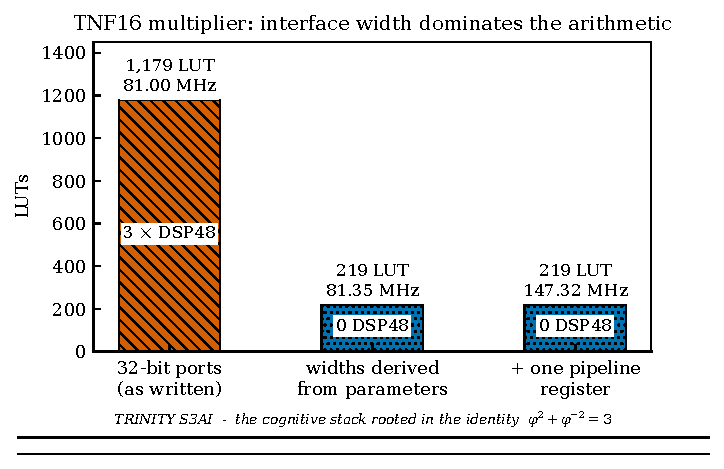
\includegraphics[width=0.82\textwidth]{tnf_width.pdf}
\caption{The same arithmetic at three interface widths.}
\label{fig:width}
\end{figure}

\subsection{The same width decided correctness}

At TNF32 the significand product needs 52 bits. The 32-bit wire truncates, and
the module returns wrong results while appearing to support the rung, since its
own documentation names TNF32 as a supported configuration. Measured against a
64-bit reference: 1{,}995{,}730 mismatches in 2{,}128{,}964 combinations.

Deriving every width from the format parameters removes both problems at once. We
report this because the pattern is not specific to TNF: in a parametric
arithmetic core, a width that is merely \emph{large enough for the configuration
that was tested} is a silent-truncation trap at the next one, and it will not be
caught by a testbench written against the tested configuration.

\section{Equivalence}\label{sec:equiv}

Every change above is a claim that timing or width changed and arithmetic did
not. Each was checked rather than argued.

\begin{table}[t]\centering
\caption{Equivalence evidence. The reference for each rung is the module already
trusted for that rung.}
\label{tab:equiv}
\begin{tabular}{lrr}
\toprule
check & combinations / cycles & mismatches \\
\midrule
width-derived vs original, TNF16 (sweep)      & $321{,}156$   & $0$ \\
width-derived vs original, TNF4               & $374$         & $0$ \\
width-derived vs original, TNF8               & $3{,}716$     & $0$ \\
width-derived vs original, TNF16              & $77{,}444$    & $0$ \\
width-derived vs 64-bit reference, TNF32      & $300{,}000$   & $0$ \\
pipelined vs combinational                     & $199{,}994$   & $0$ \\
\midrule
original 32-bit module vs 64-bit ref, TNF32   & $2{,}128{,}964$ & $1{,}995{,}730$ \\
\bottomrule
\end{tabular}
\end{table}

The TNF16 sweep is exhaustive in the sense that matters here: the mantissa space
is covered in full at offset pairs exercising underflow, mid-range and
saturation, then the offsets are covered in full at mantissas that do and do not
carry --- every path through the carry, the saturation and the underflow clamp.
The last row is the point of the section: the width-derived module agrees with
the reference that is correct and disagrees with the one that truncates.


\section{Why ternary, and exactly how much}\label{sec:whyternary}

The case for a ternary exponent is usually made by citing radix economy and left
there. We state it, then bound it in two directions --- what a binary fabric takes
back, and what the radix of the \emph{scale} is worth as distinct from the radix
of the \emph{exponent} --- because both bounds turn out to be decisive for the
design and neither is folklore.

\begin{theorem}[Radix economy]
\label{thm:economy}
Representing $R$ distinct values in radix $b$ costs $b\log_b R = b\ln R/\ln b$
state-slots. The factor $b/\ln b$ is minimised at $b = e$; among integers it is
$3/\ln 3 = 2.731$ against $2/\ln 2 = 2.885$, so a ternary field is $5.3\%$ more
economical than a binary one.
\end{theorem}

This is the classical argument~\cite{hayes2001,radixeconomy} and it is what
motivates a ternary exponent. It is also stated in a currency --- state-slots ---
that no binary fabric pays in. The next theorem says what happens when it does.

\begin{theorem}[No free range on a binary fabric]
\label{thm:nofree}
An exponent field of $E_t$ trits spans $3^{E_t}$ values. Stored as a binary
integer it occupies $\lceil E_t\log_2 3\rceil$ bits, a field spanning
$2^{\lceil E_t\log_2 3\rceil} \geq 3^{E_t}$ values. Hence on a binary fabric a
ternary exponent never spans more values per bit than a binary one, with equality
only at $E_t = 0$. Writing $\rho(E_t) = 3^{E_t}/2^{\lceil E_t\log_2 3\rceil}$ for
the utilisation, $\rho \in (1/2, 1]$ and $\rho$ does not converge.
\end{theorem}

\begin{table}[t]\centering
\caption{Utilisation $\rho(E_t)$ of the binary field holding an $E_t$-trit
exponent. The ladder's present budgets, $E_t \in \{4, 7\}$, are the two worst
entries in the range.}
\label{tab:rho}
\begin{tabular}{lrrrrrrrrrr}
\toprule
$E_t$ & 2 & 3 & 4 & 5 & 6 & 7 & 8 & 9 & 10 & 11 \\
\midrule
$\rho$ & $56.2$ & $84.4$ & $\mathbf{63.3}$ & $94.9$ & $71.2$ & $\mathbf{53.4}$ & $80.1$ & $60.1$ & $90.1$ & $67.6$ \\
\bottomrule
\end{tabular}
\end{table}

Run as an optimisation rather than an inequality, the same statement is sharper
than it looks. Asking which exponent encoding a binary fabric prefers at
$(N, R) = (16, 24)$, $(32, 219)$ and $(64, 658)$ returns the same mantissa width
for both --- $M = 10$, $23$ and $53$ respectively. The ternary encoding does not
lose on a binary fabric; at these widths the ceilings absorb the difference and it
exactly ties, which is the strongest form of ``never more values per bit''.

Theorem~\ref{thm:nofree} is the reason the ladder's rung widths must be read as
position counts and not bit counts, and it is where our own first reading of the
ladder went wrong: measuring what a trit costs when packed into bits and calling
the result the format's width confuses a fabric cost with a format property. The
independently published balanced-ternary float Ternary27~\cite{ternary27} counts
the same way --- 2 type trits, 1 sign trit, 5 exponent trits and 19 significand
trits, exactly 27 --- which is external corroboration that position counting is
the convention in this family rather than a reading of our own.


The final question is one the ladder answers implicitly and, as far as we can
find, no one has stated: TNF encodes its exponent in radix 3 but scales by
$2^{e}$, whereas Ternary27 scales by $3^{e}$. These are different choices and
they are separable.

\begin{theorem}[The scale radix, and why 2 beats 3]
\label{thm:scaleradix}
Let a format scale by $r^{e}$ with a normalised significand uniformly quantised
over $[1, r)$ by $M$ bits. Then its expected relative error on a log-uniform
workload is $\kappa(r)\,2^{-M}$ with
\[
\kappa(r) \;=\; \frac{(r-1)^{2}}{r\ln r},
\qquad \kappa(2) = 0.72135,\quad \kappa(3) = 1.21365 .
\]
Holding the field layout fixed, moving the scale from $r=2$ to $r=3$ therefore
multiplies the error by $\kappa(3)/\kappa(2) = 1.6825$ while multiplying the
dynamic range by $\log_2 3 = 1.5850$. Measured in positions, it costs
$\log_2 1.6825 = 0.7506$ of precision and buys $\log_3 1.5850 = 0.4192$ of range:
a net loss of $0.3314$ positions per number. A power-of-two scale strictly
dominates a power-of-three scale at equal width.
\end{theorem}

\begin{proof}
The quantisation step over $[1,r)$ is $(r-1)2^{-M}$ and the mean absolute
rounding error is half of it. On a log-uniform workload the significand has
density $1/(s\ln r)$ on $[1,r)$, so
$\mathbb{E}[1/s] = \frac{1}{\ln r}\int_1^{r} s^{-2}\,ds = \frac{1-1/r}{\ln r}$.
Multiplying gives $\tfrac12 (r-1)2^{-M}\cdot\frac{1-1/r}{\ln r}$, and
$\tfrac12(r-1)(1-1/r) = (r-1)^2/2r$. Absorbing the factor $\tfrac12$ into the
$2^{-(M+1)}$ convention of Theorem~\ref{thm:law} yields $\kappa$ as stated. For
the range, $E_t$ trits span $3^{E_t}$ steps of $\log_2 r$ binades each. One
mantissa bit halves the error and one exponent trit triples the range, which
fixes the exchange rate between the two currencies and gives the position
figures. \qed
\end{proof}

Direct measurement at two rungs, encoding and decoding through both scales in
exact arithmetic, gives error ratios of $1.675$ at $(E_t,M) = (4,11)$ and $1.690$
at $(6,25)$ against the predicted $1.6825$, and range ratios of $1.583$ and
$1.585$ against the predicted $1.5850$.

\begin{corollary}[What TNF is, precisely]
TNF is not a ternary float in the sense of Ternary27; it is a binary-radix float
whose exponent is \emph{encoded} in balanced ternary. Theorem~\ref{thm:scaleradix}
says that this is the better of the two available choices by $0.331$ positions per
number, and Theorem~\ref{thm:nofree} says that the ternary encoding pays only on a
ternary fabric. The two together delimit the format exactly: the radix choice is
right on any fabric, and the encoding choice is right on one.
\end{corollary}


\paragraph{And a second, independent argument for the same scale radix.} The
radix of a scale also decides how much a format's precision oscillates inside
one step of its ladder, and that quantity has a closed form. Write
$M_{\mathrm{eff}}$ for the \emph{effective mantissa} --- the mantissa width a
fixed-field format would need in order to produce the round-trip error actually
observed in a given magnitude band, which by Theorem~\ref{thm:law} is
$-\log_2\bigl(2\,\mathbb{E}[|\text{rel err}|] / \mathbb{E}[1/s]\bigr) - 1$.
The diagnostic that recovers it across a catalogue of formats is the companion
paper's; only the theorem below and the two checks it passes are needed here.

\begin{theorem}[Precision wobble]
\label{thm:wobble}
Let a format scale by $r^{e}$ with a significand quantised uniformly over a
scale interval spanning a factor $r$. Its relative error varies by a factor of
$r$ across that interval, so $M_{\mathrm{eff}}$ oscillates with amplitude exactly
$\log_2 r$ bits and has no trend in $|e|$.
\end{theorem}

\begin{proof}
The quantisation step is constant across the interval and the relative error is
that step divided by the significand, which ranges over a factor $r$. Taking
$-\log_2$ of the ratio of the extremes gives $\log_2 r$. Since the interval
repeats identically at every $e$, the oscillation is periodic and carries no
trend. \qed
\end{proof}

Theorem~\ref{thm:wobble} reproduces a result sixty years older than this work.
IBM System/360 hexadecimal is documented as delivering between $4p-3$ and $4p$
significant bits, a spread of three~\cite{goldberg1991,ibmhfp}; the integer count
is the floor of the continuous quantity, so the theorem's $\log_2 16 = 4$ and the
textbook's $3$ are the same statement. Measured over eight sub-intervals ---
which by averaging within each bin predicts a reduced spread of $2.96$ rather than
the full $4$ --- \texttt{ibm\_hfp32} and \texttt{ibm\_hfp64} give $3.13$ and
$3.04$, while \texttt{binary32} and \texttt{gf32} give $0.85$ and $0.93$ against a
predicted $0.87$. Binary formats wobble by one bit; this is the familiar
$1$-bit wobble of every radix-2 float, and it is the smallest wobble any integer
radix admits. Theorem~\ref{thm:wobble} therefore supplies a second and independent
argument for TNF's binary scale, alongside the $0.331$ positions of
Theorem~\ref{thm:scaleradix} above: a radix-3 scale would wobble by $1.585$ bits
instead of $1$.

\section{Converting silicon into precision}\label{sec:convert}

Two of this paper's currencies are area and precision, and they cannot be
compared until they are one currency. They can be: at a fixed class a mantissa
bit has a marginal area, and by Theorem~\ref{thm:law} it has a known value in
accuracy. The exchange rate is stated here because the area law of the next
subsection is its derivative, and because it is the only bridge this paper has
between what a design costs and what it delivers. The uses the previous version
made of it --- pricing a regime codec in mantissa bits --- go with the companion
paper; the rate itself does not.

\begin{theorem}[Area and precision are commensurable]
\label{thm:convert}
Let $\lambda = \mathrm{d}A/\mathrm{d}M$ be the marginal area of a mantissa bit at
a given class. A regime codec costing $C$ LUTs is then equivalent to $C/\lambda$
mantissa bits of silicon, and by Theorem~\ref{thm:law} to a factor
$2^{C/\lambda}$ in accuracy at equal area.
\end{theorem}


Measuring $\lambda$ directly --- the same width-derived multiplier synthesised at
$M = 7, 9, \ldots, 25$ under one harness --- gives $285$, $372$, $443$, $567$,
$696$, $870$, $1238$ and $1683$ LUTs. The marginal cost is not constant: it rises
from $35.5$ LUTs per bit between $M{=}9$ and $M{=}11$ to $111.2$ between $M{=}21$
and $M{=}25$, so $\lambda = 48.8$ at the 16-bit class and $111.2$ at the 32-bit
one. That the marginal cost rises at all is the subject of the next subsection,
and it falsified a prediction we had registered.

\subsection{How area grows along the ladder}\label{sec:arealaw}

Theorem~\ref{thm:convert} needs $\lambda$, and $\lambda$ is a derivative of an
area law we can state. Fitting $A(M) = cM^{\alpha}$ to the eight rungs from
$M{=}7$ to $M{=}25$ gives $\alpha = 1.406$ at $R^2 = 0.984$, and combined with
Theorem~\ref{thm:law} it predicts a scaling relation:

\begin{proposition}[Error decays as a stretched exponential in area]
\label{prop:stretched}
With $\varepsilon \propto 2^{-M}$ and $A \propto M^{\alpha}$,
$\ln(1/\varepsilon) \propto A^{1/\alpha}$.
\end{proposition}

Measured over $M \in [7,25]$ --- a sixfold range of area and a $250{,}000$-fold
range of error --- the constant of proportionality holds to within $27\%$ and
drifts monotonically downward, so the relation is an approximation and we label
it a proposition rather than a theorem. The drift has a cause, and finding it
falsified a prediction we registered before synthesising.

\paragraph{The exponent is not constant, and the fit does not extrapolate.} We
predicted from the $[7,25]$ fit that the reconciled TNF64, at $M = 56$, would
cost $4{,}762$ LUTs. It costs $7{,}479$ at $48.20$\,MHz --- the prediction is low
by $1.57\times$. Reading $\alpha$ locally rather than globally shows why: it rises
monotonically, from $1.06$ between $M{=}7$ and $M{=}9$ to $1.78$ between $M{=}15$
and $M{=}17$ and $1.85$ between $M{=}25$ and $M{=}56$.

\begin{theorem}[The ladder's area law]
\label{thm:alpha}
A rung's area is a fixed overhead --- registers, the exponent adder, the
renormalisation --- plus a significand multiplier quadratic in $M$:
\[
A(M) \;=\; f + cM^{2}.
\]
Consequently the effective power-law exponent
$\alpha(M) = \mathrm{d}\ln A/\mathrm{d}\ln M$ is not a constant but rises
monotonically toward $2$, and the marginal cost of a mantissa bit,
$\lambda = \mathrm{d}A/\mathrm{d}M = 2cM$, is \emph{linear} in $M$ rather than
fixed.
\end{theorem}

Synthesising the same width-derived multiplier at fourteen mantissa widths from
$M{=}7$ to $M{=}90$ --- $285$, $372$, $443$, $567$, $696$, $870$, $1238$, $1683$,
$2601$, $3990$, $5934$, $7479$, $12232$ and $19980$ LUTs --- and fitting both
parameters gives $f = 141$ LUTs and $c = 2.4455$ LUTs per bit squared at
$R^2 = 0.99963$, with a maximum deviation of $9.9\%$ across a seventyfold range of
area. Read locally, $\alpha$ climbs from $1.06$ between $M{=}7$ and $M{=}9$ to
$2.20$ between $M{=}56$ and $M{=}70$, which is Theorem~\ref{thm:alpha} rather than
noise. On the registered prediction the structural model is right to $+4.4\%$
where the single power law was low by $36.3\%$; we report both, since the power
law was ours and we published the prediction before synthesising.

\section{Is there an optimal format, and what its statement was missing}
\label{sec:optimal}

The results above are individually bounding: each says what a format cannot have,
or what a claim may not be extended to. Read together they reduce the design
space, and the previous version of this paper read them as reducing it to the
point of determination. This section keeps the reduction that survives and
corrects the statement that does not, because the parameter the corrected
statement is missing is this paper's headline.

\begin{theorem}[The binary scale is the unique implementable optimum]
\label{thm:radixopt}
Let a format scale by $r^{e}$. Scaling is a shift --- and therefore free of any
polynomial or table --- if and only if $r = 2^{k}$ for integer $k \geq 1$. On
that set $\kappa(r) = (r-1)^2/(r\ln r)$ is strictly increasing, taking $0.7213$,
$1.6230$, $2.9455$ and $5.0720$ at $r = 2, 4, 8, 16$. Hence $r = 2$ minimises the
expected relative error among all radices whose scaling is implementable without
a transcendental, and it does so uniquely.
\end{theorem}

\begin{figure}[t]\centering
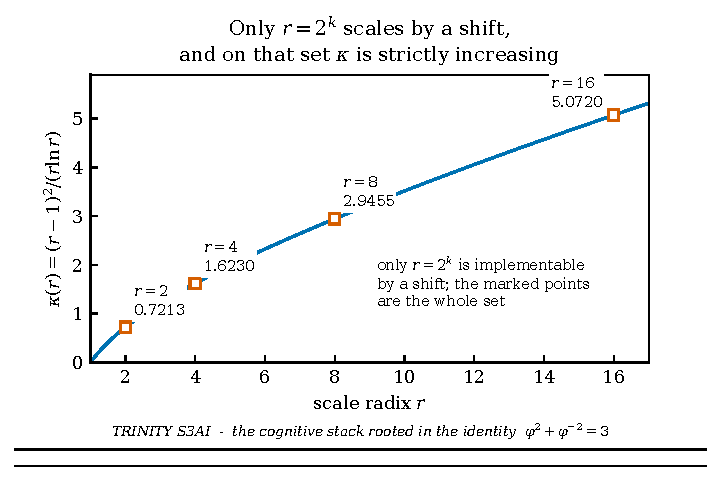
\includegraphics[width=\linewidth]{tnf_radix.pdf}
\caption{$\kappa(r)$ against the scale radix. The unconstrained minimiser sits
near $r = 1.9$ and is unreachable: only $r = 2^{k}$ scales by a shift, and on that
set $\kappa$ is strictly increasing.}
\label{fig:radix}
\end{figure}

The claim is verified by enumeration rather than resting on the monotonicity of
$\kappa$ alone. Sweeping $r$ continuously over $[1.1, 16]$ with $E$ integral and
$M$ taking the remaining width, at eight combinations of width and required range
from $(P,R) = (8, 24)$ to $(32, 5925)$, the best implementable radix is $r = 2$ in
every case, and the penalty against the unreachable optimum is $1.09\times$ at all
eight --- a constant, as it must be, since the two differ only by
$\kappa(1.9)/\kappa(2)$. The unconstrained minimiser is not $2$: it is near
$1.9$, worth $7.9\%$ in error, and it is unavailable because any $r \neq 2^{k}$
makes $r^{e}$ a transcendental evaluation whose decode costs a table.
Theorem~\ref{thm:radixopt} is therefore the interesting kind of optimality
result: the optimum is not the extremum, it is the best point that can be built.

Two scopes must be kept apart, and conflating them is a mistake this paper made.
Theorem~\ref{thm:radixopt} is about the scale radix of a \emph{number format},
where the scale is applied to every value and is decoded on the critical path of
every read. It is not about the base of a \emph{shared block scale}, which is
applied once per thirty-two weights and which Section~\ref{sec:hierarchy} prices
by a different cost model entirely --- one under which $\sqrt2$ and $2^{2/3}$ are
free. The two results happen to agree, and the agreement is corroboration rather
than evidence.

\subsection{The corollary was incomplete, and the missing input is the headline}
\label{sec:threeparams}

The previous version closed this chapter with a corollary it called \emph{three
inputs determine the format}: name the fabric, the required range, and which side
of the fixed-field/taper dichotomy the workload sits on, and the layout follows.
The three inputs are real and each is still supported:

\begin{enumerate}[leftmargin=*,itemsep=2pt]
\item \emph{Radix of the scale.} Fixed at $2$ by Theorem~\ref{thm:radixopt},
unconditionally, for a per-value scale.
\item \emph{Radix of the exponent's encoding.} Fixed by the fabric.
Theorem~\ref{thm:nofree} shows a ternary exponent never spans more values per bit
than a binary one when packed into bits, so it pays on a ternary fabric and
nowhere else.
\item \emph{The split between $E$ and $M$.} Determined once a required range is
named, by Theorem~\ref{thm:law} --- and \emph{only} then, since the error depends
on $M$ alone and the range on $E$ alone.
\end{enumerate}

\begin{corollary}[The corollary was incomplete]
\label{cor:determined}
The three inputs above determine the \emph{element}: its scale radix, its
exponent encoding, and the split between exponent and mantissa. They do not
determine a format deployed as a block. A shared scale has a fourth parameter ---
where its ladder's window sits relative to the element format's largest
magnitude --- and none of the three fixes it, because in a per-tensor format
there is no such parameter to fix. It appears only when a scale is shared.
\end{corollary}

The omission was structural rather than careless, which is why it is worth
stating as a corollary rather than as an erratum: the three inputs were derived
for a format whose scale lives inside the word, and the parameter they miss
exists only for a format whose scale does not. Corollary~\ref{cor:escape} below
names that class exactly --- a format escapes the position budget of
Theorem~\ref{thm:budget} by putting its scale outside the word --- so the paper
already contained the reason its own optimality statement would be incomplete
there, and did not carry it across.

The size of the omission is measured rather than argued.
Section~\ref{sec:alignment} sweeps the fourth parameter with the element format,
the block size and the scale-field width all held constant, and it moves
perplexity by $2.78$ on SmolLM2-135M and $0.51$ on Qwen2.5-0.5B at a single
shared constant. That is larger than any effect the three named inputs produce on
the same axis, and it is available at the cost of one comparison in a scale-
selection path that already computes the exponent.

\begin{corollary}[What this makes TNF]
\label{cor:whatitmakes}
For the arguments (ternary fabric; a range the workload actually visits; fixed
fields), the three inputs return a binary-radix float with a balanced-ternary
exponent field and a uniform mantissa split by $M = N - 1 - E_t$. That is TNF,
and on those arguments it is forced rather than designed. It follows that TNF
carries no claim off them --- in particular none on a binary fabric, where input
2 returns a binary exponent instead, and none about a shared block scale, where
Corollary~\ref{cor:determined} says the inputs are not a complete specification.
\end{corollary}

\subsection{Which first principles}
\label{sec:principles}

The width rule has been stated as a rule. It is not one: it is the solution of a
constrained maximisation, and naming the constraint is what makes the rest of the
paper follow rather than accumulate.

\paragraph{The rule is a Karush--Kuhn--Tucker condition.} Write the design problem
directly. Maximise precision subject to a position budget and a range that must be
covered:
\[
  \max_{E,M} \; M
  \quad\text{s.t.}\quad
  1 + E + M = N,
  \qquad
  r^{E} \ge b+1 .
\]
With multipliers $\lambda$ on the budget and $\mu$ on the range,
$\mathcal{L} = M + \lambda(N-1-E-M) + \mu\bigl(E - \log_r(b+1)\bigr)$ gives
$\partial_M \mathcal{L} = 1-\lambda = 0$ and $\partial_E \mathcal{L} = -\lambda+\mu = 0$,
so $\lambda = \mu = 1$. Because $\mu > 0$, complementary slackness makes the range
constraint \emph{active}: at the optimum the exponent is exactly as wide as the
range demands and not one position wider. That statement is
Theorem~\ref{thm:optimal}, now derived rather than asserted. The multiplier is
also the shadow price, and $\lambda = 1$ says a position of exponent costs exactly
a position of mantissa --- the exchange rate is unity because the budget is linear.

\paragraph{Why three and not two is a 1950s result, not ours.} The radix economy
$\rho(r) = r/\ln r$ is minimised at $r = e$. Ternary sits $0.46\%$ above that
optimum and binary $6.15\%$ above it. We claim no credit for this; what the present
work contributes is where it applies, which turns out to be the whole
reconciliation of our two axes:
\[
  \underbrace{r}_{\text{cost per position}} \times \underbrace{\log_r V}_{\text{positions}} .
\]
The number axis counts only the second factor, and there $\log_3$ against $\log_2$
gives the slack $0.3691\,E$ of Corollary~\ref{cor:slack} unconditionally. The
silicon axis restores the first factor, and packing a trit into binary fabric
charges $\kappa(3)/\kappa(2) = 1.68$ per position, which is why BNF16 and TNF16
synthesise within $1\%$ of one another. Theorem~\ref{thm:nofree} and
Corollary~\ref{cor:slack} are not in tension: they are the two factors of one
product, reported separately.

\paragraph{What is derivation and what is only resemblance.} Two connections are
literal and are used as such: the multiplier argument above, and radix economy,
which fixes the exponent's radix. A third --- Kraft's inequality, which bounds
how gently any unbounded-range format may taper --- is used in the companion
paper and is cited here only where a claim of ours has to be bounded by it. Two
resemblances are worth naming only so they are not mistaken for arguments. The
variational form recalls least action, but there is no time and no trajectory
here --- the problem is a static optimisation, and the resemblance carries no
consequence. And $1+E+M=N$ is a budget, not a conservation law: positions are
allocated by a designer, not withheld by nature. We state the distinction because
a physical-sounding derivation would be doing rhetorical work that the multiplier
argument already does honestly.

\paragraph{Where the multiplier argument was pushed too far, and is withdrawn.}
An earlier version applied the same argument to the block axis and reported that
the width rule returns the MX element for any design protecting the 90th
percentile of blocks or more. The arithmetic is unchanged and the percentile
table it rested on is not disputed. What is withdrawn is its standing as a
derivation of the deployed format: Section~\ref{sec:blockbound} shows the element
axis is closed by a margin under one percent that is itself a property of a
normalisation nobody had named, and Section~\ref{sec:alignment} shows the
parameter that actually moves a block format is not on the element at all. A
derivation that returns the right element for a reason that is not the operative
one is a coincidence with a proof attached, and we retire it rather than quote
it.

\subsection{The width rule is an optimisation with one solution}
\label{sec:widthrule}

Theorem~\ref{thm:coverage} compares against a given competitor. Stated as a
design problem it selects a member outright, which is what makes the rule
falsifiable: it names a winner before any measurement.

\begin{theorem}[Optimal member for a named range]
\label{thm:optimal}
Let a workload visit $b$ binades. Among all members of $\mathcal{F}_N$ that
represent it without overflow, the effective mantissa is maximised uniquely at
\[
  E_t^{*} = \bigl\lceil \log_3 (b+1) \bigr\rceil,
  \qquad
  M^{*} = N - 1 - \bigl\lceil \log_3 (b+1) \bigr\rceil .
\]
\end{theorem}
\begin{proof}
Representability requires $3^{E_t}-1 \ge b$, i.e.\ $E_t \ge \log_3(b+1)$, and
$E_t$ is an integer, so $E_t \ge E_t^{*}$. By the width rule $M = N-1-E_t$ is
strictly decreasing in $E_t$, so the constraint binds and the minimiser is unique.
\end{proof}

The rule therefore has no free parameter once the workload is named, and naming
the workload is a measurement rather than a choice. It is used that way below:
the binade span of a network's weights is measured first, the optimum is computed
from it, and only then is perplexity evaluated. A different winner would falsify
the rule, and in Section~\ref{sec:blockbound} one did.

\begin{theorem}[Regret of a misnamed range]
\label{thm:regret}
Sizing for $b'$ when the workload visits $b$ costs
\[
  R =
  \begin{cases}
    \lceil\log_3(b+1)\rceil - \lceil\log_3(b'+1)\rceil \ \text{mantissa bits}, & b' > b,\\[2pt]
    \text{overflow on a set of measure } 1 - \tfrac{\log_3(b'+1)}{\log_3(b+1)}, & b' < b .
  \end{cases}
\]
The penalty is asymmetric: over-sizing costs precision logarithmically, under-sizing
costs range linearly, so when the visited range is uncertain the rule should round up.
\end{theorem}

The asymmetry is worth naming because it contradicts the intuition that a wider
exponent is the conservative choice. It \emph{is} conservative --- but the price is
paid in every value the format ever represents, whereas the price of being too
narrow is paid only on the tail. Which dominates is an empirical question about
the tail's weight, not a matter of taste.

\paragraph{And the asymmetry now has an instrument.} Theorem~\ref{thm:regret} was
stated and never measured; Section~\ref{sec:cliff} measures it. Sweeping the
alignment of a shared block scale walks the under-sizing branch directly, and the
response has exactly the predicted shape: a long shallow decline where range is
over-provisioned and precision is being wasted on every value, then a steep rise
past the optimum where range runs out and the cost falls on the tail. On
SmolLM2-135M the shallow side spans $2.02$ perplexity across seven sampled
alignments and the steep side spans $11.15$ across four. The deployed constant
of the MX specification sits on the steep side.

\begin{corollary}[When the trit is worth its packing]
\label{cor:worth}
Ternary buys $\Delta = E(1-\log_3 2)$ positions and costs
$\kappa(3)/\kappa(2) = 1.683$ per position when packed into binary fabric, where
$\kappa(r) = (r-1)^2/(r \ln r)$. The two cancel at $E$ satisfying
$\Delta = 0.331\,E_t$, so on positions the trit wins outright and on binary bits
it breaks even --- which is why BNF16 and TNF16 synthesise within $1\%$ of one
another while the number-axis frontier separates them.
\end{corollary}


%% ===================== PART B: the ternary node =====================

\section{Two formats close a ternary node}
\label{sec:pair}

A ternary node contains exactly three sites where a number format could live, and
only one of them needs one.

\begin{enumerate}
\item The \textbf{weight} is a code. Multiplying by it is a sign-select
      ($+x$, $-x$, $0$), not a multiply.
\item The \textbf{sample} arrives ADC-native and is used as it lands.
\item The \textbf{accumulator} is the only object in the system carrying a
      dynamic range that must be spent.
\end{enumerate}

This is the whole design problem, and it is smaller than the literature makes it
look. The published ternary methods --- BitNet-style, with weights in
$\{-1,0,+1\}$~\cite{bitnet} --- answer (1) and leave (3) in \texttt{fp16} or
\texttt{int8}; the published format work answers (3) and assumes a multiplier at
(1). We answer both --- but not with the two objects the previous version named.

The previous version answered (3) with a float ladder, and our own measurement
narrows that. Section~\ref{sec:exact} shows that the closed linear path
accumulates exactly in a pair of $32$-bit integers with eleven bits of headroom
against a worst case that is attained rather than estimated, so what site (3)
wants at inference is an accumulator \emph{width}, not a ladder. A ladder is
wanted at (3) only where the range crossing the accumulator cannot be predicted
in advance, which is the training-side case and not the one measured here. The
honest statement of the pair is therefore: \emph{an alphabet and an accumulator
width close a ternary node at inference}, and the format the previous version was
named after is scoped to the sites where a width is not enough.

\subsection{Why the weight alphabet is \texorpdfstring{$\varphi$}{phi}, and why that is forced}

GFTernary is a two-bit alphabet $\{-\varphi,\,0,\,+\varphi\}$. The $\varphi$ is
not decoration, and the following says why --- with the hypotheses it needs named
in the statement, because the previous version left one of them implicit and a
later result exposed it.

\begin{theorem}[The golden alphabet is the unique degree-two choice]
\label{thm:goldalpha}
Let a three-symbol weight alphabet be $\{-r,0,+r\}$ with $r>1$, and require that
the product of two weights be expressible in the additive lattice the datapath
already computes in, \emph{at degree two and with unit coefficients}, i.e.\
$r^2 = r + 1$. Then $r = \varphi$ uniquely.
\end{theorem}
\begin{proof}
$r^2 - r - 1 = 0$ has roots $(1\pm\sqrt5)/2$, of which one is positive.
\end{proof}

\paragraph{The hypotheses are load-bearing, and Section~\ref{sec:hierarchy}
supersedes this theorem as a uniqueness argument.} Written as above, the
uniqueness is uniqueness \emph{given} the recurrence $r^{2}=r+1$, and that
recurrence was chosen rather than derived. The classification of
Section~\ref{sec:sparsemult} replaces the choice with a cost model: applying
$r^{k}$ costs one add/subtract exactly when some monic annihilator of $r$ has
non-leading weight two, and under coefficients in $\{0,\pm1\}$ every such ratio
in $(1,2)$ is at most $\varphi$ (Theorem~\ref{thm:t6}). $\varphi$ is therefore
the largest one-adder ratio rather than the only lattice-closing one, and
Theorem~\ref{thm:goldalpha} is retained as the degree-two case rather than as the
general argument. What is \emph{not} superseded is the alphabet result of
Section~\ref{sec:closure}: a ratio can be cheap to apply and still fail to close
the weight lattice --- $\sqrt2$ satisfies $r^{2}=2$ at zero adders and loses the
scale out of the lattice entirely --- so cheapness on the scale axis and closure
on the alphabet axis are different requirements and $\varphi$ is chosen here for
the second.

\begin{corollary}[Depth costs no multiplier]
\label{cor:depth}
The gain of a stack of $k$ ternary $\varphi$-layers is exactly
\[
  \varphi^{k} = F_k\,\varphi + F_{k-1},
\]
a pair of integers with $F$ the Fibonacci sequence. Rescaling between layers is
therefore a shift-and-add, and the zero-multiplier property survives to arbitrary
depth.
\end{corollary}

This is the practical content of Theorem~\ref{thm:goldalpha}, and it is what
separates the $\varphi$ alphabet from the $\{-1,0,+1\}$ one used throughout the
ternary-network literature. With unit weights the layer gain is $1$ and carries no
information, so every published method attaches a learned real scale $\alpha_\ell$
per layer --- and multiplying by $\alpha_\ell$ puts the multiplier back. With the
$\varphi$ alphabet the inter-layer scale is known exactly and is a pair of
integers, so it is never multiplied by. Storage is two bits either way and the
symbol count is three either way; the $\varphi$ alphabet simply carries a scale
that the unit alphabet has to learn and then pay for.


\subsection{The linear path is exact, and what that is worth}
\label{sec:exact}

On the alphabet it fixes, the $\varphi$ datapath computes its entire linear part
without rounding. We state this carefully, because the obvious reading of it is
wrong and we published that reading once already
(Section~\ref{sec:scaleapplier}).

Exactness is not something $\varphi$ has and binary formats lack. Every
\texttt{int8} network on every deployed accelerator accumulates exactly, in an
\texttt{int32} register; an APoT scale is a dyadic rational and $\mathbb{Z}[1/2]$
is a ring under the same operations. What is special about $\varphi$ is
narrower and runs the other way. A scale ladder with an \emph{irrational} ratio
would generically destroy exactness --- the levels are not integers, so an
integer accumulator cannot hold their sum. $\varphi$ is the case where it
survives anyway, because $\mathbb{Z}[\varphi]$ is a rank-two ring: the price is a
second integer register and the benefit is that the irrational ladder costs no
rounding. That is the whole claim of this subsection. Everything else here is
the price, measured.

Represent a value as an integer pair $(a,b)$ standing for $a + b\varphi$. Then
\[
  \varphi\,(a + b\varphi) \;=\; a\varphi + b\varphi^{2} \;=\; a\varphi + b(\varphi+1)
  \;=\; b + (a+b)\varphi ,
\]
so applying a weight is the map $(a,b) \mapsto (b,\,a+b)$ --- the Fibonacci
recurrence, one integer addition, no shift. Negation flips both components and a
zero weight is a skip.

\begin{theorem}[Exactness of the multiply-free path]
\label{thm:exact}
Let $\mathbb{Z}[\varphi] = \{a + b\varphi : a,b \in \mathbb{Z}\}$. Then
\begin{enumerate}[label=(\roman*),topsep=2pt,itemsep=1pt]
\item $\mathbb{Z}[\varphi]$ is a ring: closed under addition, negation and
      multiplication;
\item the weight alphabet $\{-\varphi,0,+\varphi\}$ lies inside it, and applying
      a weight is the integer map $(a,b) \mapsto \pm(b,\,a+b)$, or the zero map;
\item consequently, for inputs in $\mathbb{Z}[\varphi]$ the entire linear part of
      a ternary network --- every weight application and every accumulation, to
      arbitrary fan-in and arbitrary depth --- remains in $\mathbb{Z}[\varphi]$
      and is computed without rounding error, given unbounded integers.
\end{enumerate}
\end{theorem}
\begin{proof}
(i) Closure under addition and negation is componentwise; closure under
multiplication follows from $\varphi^{2} = \varphi + 1$, which reduces
$(a+b\varphi)(c+d\varphi)$ to $(ac+bd) + (ad+bc+bd)\varphi$. (ii) is the
displayed identity with $\varphi = 0 + 1\!\cdot\!\varphi$. (iii) is induction over
the operations of the linear path, each of which is one of (i) or (ii).
\end{proof}

\paragraph{Attribution.} Nothing in Theorem~\ref{thm:exact} is new mathematics.
$\mathbb{Z}[\varphi]$ is the ring of integers of $\mathbb{Q}(\sqrt5)$, and
representing quantities on a $\varphi$ ladder by Fibonacci pairs goes back to
Bergman's irrational-base number system~\cite{bergman1957} and Zeckendorf
representation~\cite{zeckendorf1972}. Fibonacci \emph{weight} encoding for neural
hardware is Simon et al.~\cite{simon}, and the arithmetic consequences of a
Fibonacci alphabet are worked out in FQP~\cite{fqp} and in fibbinary
quantization~\cite{fibbinary}; Section~\ref{sec:closure} is where we compare
against them, and the difference is closure, not the ladder. We state the
theorem because the rest of Part~B is provisioned from it, and because it is what
makes the accumulator width a measurable quantity rather than a design margin.

\paragraph{What is machine-checked, exactly.} The algebraic core,
$\varphi^{2} = \varphi + 1$ on the reals, is proved in Coq with no admitted
lemmas (\texttt{Kernel/Phi.v}, lemma \texttt{phi\_squared\_identity}). The
datapath-level statement --- that the map $(a,b)\mapsto(b,a+b)$ carries an entire
dot product without error --- is \textbf{not} in a proof assistant; a previous
draft said it was, and that claim is withdrawn. It is checked numerically, by
three oracles that test different things:
$\varphi^{m} = F_m\varphi + F_{m-1}$ to better than $10^{-45}$ relative over
$m = 0\dots200$ in $60$-digit decimal; the block-scale bracket recomputed in
exact $\mathbb{Z}[\varphi]$ and \texttt{Fraction} arithmetic on every
near-boundary block; and an \texttt{int64} vectorised accumulation required to
agree \emph{bitwise} with an arbitrary-precision integer accumulation on real
(tensor, row, token) triples across twelve tensors. A negative control runs with
them: corrupting one Fibonacci table entry, $F_5$, must break the identity, and
does.

\subsubsection*{The width claim, corrected}

v1 said the component widths ``grow logarithmically, reaching eight bits over
$512$ terms'', and provisioned hardware from the triangle inequality over partial
sums,
\begin{equation}
  W \;=\; \bigl\lceil \log_{2}\!\bigl(n\,A\,\max(F_S,1)\bigr) \bigr\rceil + 1 ,
  \label{eq:wcbound}
\end{equation}
with $n$ the fan-in, $A$ the activation bound and $S$ the $\varphi$-span of the
weights inside one accumulation. At $n=512$, $A=127$, $S=43$ this is $46$ bits
per component. Both are wrong, in opposite directions: eight bits understates the
measurement by eleven, and $46$ charges for something the datapath does not pay
for.

\begin{theorem}[A $W$-bit datapath returns the exact answer modulo $2^{W}$]
\label{thm:modw}
Componentwise addition, the Fibonacci step $(a,b)\mapsto(b,a+b)$ and
multiplication by an integer are all $\mathbb{Z}$-linear maps on the coordinate
pair, so each is given by an integer matrix. Reduction modulo $2^{W}$ is a ring
homomorphism $\mathbb{Z} \to \mathbb{Z}/2^{W}\mathbb{Z}$ and commutes with such a
map. A $W$-bit two's-complement datapath therefore holds, at every step, the
exact value of that step reduced mod $2^{W}$; the final pair is exact if and only
if both components lie in $[-2^{W-1},\,2^{W-1})$, whatever the partial sums did
on the way.
\end{theorem}

\paragraph{This is a rediscovery, and its preconditions are not free.} That a
wrapping two's-complement accumulator returns the correct sum whenever the
\emph{result} is in range is standard computer arithmetic~\cite[Sec.~4.3.1]{knuth2}
and standard fixed-point DSP practice; Theorem~\ref{thm:modw} is that fact
transported to a rank-two coordinate ring, and we claim only the transport. It
buys nothing unless three conditions hold, and each is a real constraint on an
implementation: the adders must \emph{wrap}, not saturate --- a saturating
accumulator, which is the DSP default, destroys the cancellation; no comparison,
shift-right, rounding or clamp may sit inside the accumulation, which forbids
folding an activation function or a running max into the loop; and both
components must fit, not just the one that is checked.

\begin{corollary}[The provisioning rule is sufficient; it is tight only at small fan-in]
\label{cor:suffnotnec}
Bound~\eqref{eq:wcbound} dominates every partial sum, so it always suffices. It
is not necessary in general, because intermediate overflow in a wrapping
$\mathbb{Z}[\varphi]$ datapath is self-cancelling and the accumulator must be
sized to the \emph{answer}. How loose it is depends on how much cancellation the
sum offers, which is a property of the fan-in: Table~\ref{tab:accwidth} shows the
attained worst case falling $4$ bits below the bound at fan-in $512$ and
\emph{equalling} it at fan-in $8$, $16$ and $32$, where a single quantisation
block leaves nothing to cancel. A bit-accurate two's-complement simulation run at
widths below~\eqref{eq:wcbound} returned the exact final pair in twelve of twelve
trials, six of them after a genuine intermediate overflow that cancelled; those
trials test the simulator against Theorem~\ref{thm:modw}, they are not evidence
for it.
\end{corollary}

The bound is therefore a design constant only where it is tight, and elsewhere it
is a question. The final value is a \emph{signed} sum with cancellation and has
no reason to sit near $46$ bits, so we measured it.

\begin{table}[t]\centering
\caption{Final-pair width, signed two's complement, worst of the two components.
SmolLM2-135M, all $210$ \texttt{nn.Linear} tensors (\texttt{lm\_head} is tied and
excluded), weights on the campaign's $\varphi^{k}$ grid --- block $32$ along
\texttt{in\_features}, block scale $\varphi^{\lceil\log_\varphi a_{\max}\rceil}$,
ladder $\varphi^{-6}\dots\varphi^{0}$ --- so every nonzero weight is exactly
$\pm\varphi^{m}$. \textbf{Two different arms.} Columns p50/p99/max are the
\emph{real}-activation arm: inputs to each \texttt{Linear} captured from an
\texttt{fp32} forward pass on wikitext-2 and quantised per token, symmetric, to
\texttt{int8}, at $T$ token positions per layer ($T$ in the second column;
$T\!=\!2$ for the sweep rows is a thin sample and their max should be read as a
lower bound on the real-activation maximum). The ``worst'' column is a separate
arm over $328{,}320$ row-tiles ($155{,}520$ rows for the whole-row line) with no
token sampling at all: $m_{\min}$ normalisation makes every Fibonacci coefficient
non-negative, so $x_j = 127\,\mathrm{sign}(s_j)$ \textbf{attains} the maximum over
all \texttt{int8} vectors exactly. Eleven all-zero tiles at fan-in $8$ carry no
accumulation and are excluded ($11$ tiles $\times\,2$ tokens $=22$, which is the
shortfall from $26{,}542{,}080$); at every other fan-in there are none. Measured,
with one exception: $^{\dagger}$ is derived. The harness
evaluates~\eqref{eq:wcbound} at its configured $n=512$ and stores $25$ for the
whole-row line too; a whole-row accumulation on this model runs to $n=1536$, and
$\lceil\log_2(1536\cdot127\cdot F_{13})\rceil+1 = 27$ is the honest bound for it.
Table~\ref{tab:spanorigin} keeps the harness convention, which is why its
whole-row entry reads $25$.}
\label{tab:accwidth}
\begin{tabular}{lrrrrrrr}
\toprule
& & \multicolumn{4}{c}{real \texttt{int8} activations} & worst over & bound \\
\cmidrule(lr){3-6}
fan-in $n$ & $T$ & accumulations & p50 & p99 & max & all \texttt{int8} & \eqref{eq:wcbound} \\
\midrule
$8$        & $2$   & $26{,}542{,}058$ & $6$  & $10$ & $13$ & $\mathbf{14}$ & $14$ \\
$16$       & $2$   & $13{,}271{,}040$ & $7$  & $10$ & $13$ & $\mathbf{15}$ & $15$ \\
$32$       & $2$   & $6{,}635{,}520$  & $8$  & $11$ & $14$ & $\mathbf{16}$ & $16$ \\
$64$       & $2$   & $3{,}317{,}760$  & $9$  & $12$ & $15$ & $17$ & $22$ \\
$128$      & $2$   & $1{,}797{,}120$  & $9$  & $12$ & $16$ & $19$ & $23$ \\
$256$      & $2$   & $1{,}036{,}800$  & $10$ & $13$ & $18$ & $20$ & $24$ \\
$512$      & $128$ & $42{,}024{,}960$ & $11$ & $14$ & $19$ & $\mathbf{21}$ & $25$ \\
whole row  & $32$  & $4{,}976{,}640$  & $11$ & $14$ & $19$ & $22$ & $27^{\dagger}$ \\
\bottomrule
\end{tabular}
\end{table}

\paragraph{Thirty-two bits, with eleven to spare.} At the operating fan-in of
$512$, the widest final pair over $42{,}024{,}960$ real accumulations is $19$
bits, and the widest \emph{attainable} over every \texttt{int8} activation vector
is $21$. A signed $32$-bit component carries $11$ bits of headroom against a
worst case that is reached, not estimated. Converting that headroom into fan-in
requires the conservative route, since the attained maximum is a property of
these weights and does not extrapolate: at the measured worst per-accumulation
span $S=13$ a single term contributes at most $127F_{13} = 29{,}591$, so a signed
$32$-bit component admits $\lfloor (2^{31}-1)/29{,}591 \rfloor = 72{,}572$ such
terms while still satisfying~\eqref{eq:wcbound}, about $142\times$ the fan-in in
use. Derived from the measured span, not measured.

Two variants, both on the worst-case arm so they are comparable with its column
and not with p99 of the real arm. Accumulating a whole row in one shot rather
than in $512$-term tiles costs one bit: $22$ against $21$. Referencing the pair
to one exponent per tensor rather than one per tile --- which removes a per-tile
constant from the control path --- costs three more: worst case $24$, p99 $22$,
and no row of any tensor above $32$.

\paragraph{Sixteen bits, and exactly where it stops.} The assembled ternary
neuron of Table~\ref{tab:node} is built at fan-in $8$, $16$ and $32$ on a $16$-bit
datapath, and that choice is exact there for a structural reason, not a lucky
measurement. A tile of $32$ or fewer contraction terms lies inside one
quantisation block, and the ladder has seven rungs, so $d_j \in [0,6]$ and
$S \le 6$ by construction; the largest component any \texttt{int8} vector can
produce is $32 \cdot 127 \cdot F_6 = 32{,}512 < 2^{15}$. No activation vector
exists that wraps a $16$-bit pair at those fan-ins, on any checkpoint with this
element format. The margin is $256$, under one percent, and it stops immediately
after: at fan-in $256$, four of $1{,}036{,}800$ real accumulations exceed $16$
bits; at $512$, $669$ of $42{,}024{,}960$ do, a fraction of $1.6\times10^{-5}$.
This is the failure mode Section~\ref{sec:width} records, on a different unit: a
width that is provably exact for the configuration in hand is silently wrong one
step out.

\paragraph{Where the span comes from --- measured, with one variable too many.}
\begin{table}[t]\centering
\caption{Same $210$ SmolLM2-135M tensors, same weights, two grids. The single
global grid takes $m = \operatorname{round}(\log_\varphi |w|)$ on every nonzero
weight; the campaign grid takes $m = e_{\text{block}} + \text{ladder index} - 7$
on the nonzero codes. Rows are row-tiles. The bound column
evaluates~\eqref{eq:wcbound} at $n=512$, $A=127$ and that span, for every line
including the whole-row ones (see Table~\ref{tab:accwidth}, note $\dagger$).
Measured. \textbf{The two grids differ in two ways at once} --- the global grid
has neither a per-block scale nor the seven-rung ladder floor --- so this
measures their joint effect and does not separate them. It does settle which of
the two spans, $13$ and $43$, belongs to which grid.}
\label{tab:spanorigin}
\begin{tabular}{llrrrrr}
\toprule
grid & accumulation & rows & p50 & p99 & max & bound \\
\midrule
campaign, block $32$ + ladder & $512$-tile & $328{,}320$ & $7$  & $9$  & $\mathbf{13}$ & $\mathbf{25}$ \\
campaign, block $32$ + ladder & whole row  & $155{,}520$ & $7$  & $9$  & $\mathbf{13}$ & $\mathbf{25}$ \\
\addlinespace
single global $\varphi^{k}$ grid & $512$-tile & $328{,}320$ & $16$ & $25$ & $43$ & $46$ \\
single global $\varphi^{k}$ grid & whole row  & $155{,}520$ & $16$ & $26$ & $43$ & $46$ \\
\bottomrule
\end{tabular}
\end{table}

\paragraph{The element format is the enabling condition, not only an accuracy
device.} On the unblocked, unfloored grid a \emph{single} term reaches
$127F_{43} = 55{,}053{,}793{,}499$, needing $36$ magnitude bits and $37$ signed:
a $32$-bit component cannot hold one term, let alone $512$ of them. The
element-and-scale machinery of Part~C is therefore a precondition for the
arithmetic of Part~B and not a consumer of it --- the join between the two halves
of the paper runs in the direction one would not guess. Measured, and attributed
jointly: Table~\ref{tab:spanorigin} varies the block scale and the ladder floor
together, so we can say the pair of them collapses the span from $43$ to $13$ and
cannot say which does how much.

\subsection{What exactness buys, measured}
\label{sec:exactbuys}

An exact accumulator is not a more accurate accumulator. \texttt{float32}
accumulation is unbiased around the exact answer, so removing its error removes
\emph{scatter} and leaves the mean where it was. The claim is worth what the
scatter is worth, and the scatter is measurable.

Two arms, identical in every other respect: every \texttt{nn.Linear} computes its
dot product either in \texttt{float32}, or in \texttt{float64} rounded once to
\texttt{float32}. This second arm is a \textbf{proxy} for the
$\mathbb{Z}[\varphi]$ accumulator, not the accumulator itself --- the integer
pair path is validated separately and bitwise, but on twelve tensors, not on a
whole model. The proxy is a good one and its residual is quantified: a product of
two \texttt{float32} values is exact in \texttt{float64} ($24+24 \le 53$ bits),
and a few thousand such products accumulate with relative error $\sim10^{-16}$,
about $10^{-9}$ of a \texttt{float32} ulp. It is therefore exact-then-rounded to
within one part in $10^{9}$ of the rounding decision, which is not the same as
order-independent, and Table~\ref{tab:payoff} measures the difference rather than
assuming it away. Weights are quantised on the pure $\varphi^{k}$ grid once, in
natural block order; every arm holds bitwise identical weight \emph{values}, and
only the contraction order and the accumulator differ.

\begin{table}[t]\centering
\caption{The accuracy payoff of exactness. wikitext-2, $40$ windows of $2048$
tokens, $\varphi^{k}$-quantised weights, four threads. ``Order spread'' is
$\max-\min$ over the \texttt{fp32} arm's orderings --- six on SmolLM2 (natural,
identity, reverse, three random), four on Qwen --- against \emph{two} on the
exact arm (natural, one random), so the last two columns are not sampled equally
and the matched comparison is given in the text instead. ``Payoff'' is
$\mathrm{ppl}(\text{exact}) - \mathrm{ppl}(\texttt{fp32})$ at natural order;
negative favours exactness. A plain repeat of the natural-order run reproduces it
bitwise on both models, and on SmolLM2 the identity permutation does too, so the
determinism floor is $0$. Measured.}
\label{tab:payoff}
\begin{tabular}{lrrrrr}
\toprule
model & linears & \texttt{fp32} ppl & order spread & payoff & exact arm's own \\
      &         &   (natural)       & (6 / 4 runs) &        & order effect (2 runs) \\
\midrule
SmolLM2-135M   & $210$ & $28.3289666$ & $6.75\times10^{-6}$ & $-8.44\times10^{-7}$ & $5.07\times10^{-7}$ \\
Qwen2.5-0.5B   & $168$ & $17.2704568$ & $3.10\times10^{-5}$ & $+1.05\times10^{-5}$ & $1.03\times10^{-6}$ \\
\bottomrule
\end{tabular}
\end{table}

\paragraph{The sign flips between the two models, and that is the result.}
Exactness helps SmolLM2 by $8.44\times10^{-7}$ perplexity and hurts Qwen by
$1.05\times10^{-5}$. A quantity whose sign depends on the checkpoint is the
residual of an unbiased error, not an accuracy improvement. On SmolLM2 it is not
even resolvable above the instrument, being the same size as the exact arm's own
residual order effect. We claim scatter removal and nothing else.

\paragraph{The matched comparison, since the arms are not sampled equally.}
Comparing a six-run spread against a two-run spread flatters the exact arm by
construction. On the same pair of orderings (natural against the same random
permutation) the \texttt{fp32} arm moves $4.90\times10^{-6}$ and the exact arm
$5.07\times10^{-7}$ on SmolLM2, a factor of $9.7$; on Qwen,
$2.04\times10^{-5}$ against $1.03\times10^{-6}$, a factor of $19.8$. The
conclusion survives the correction --- the exact arm is an order of magnitude
quieter --- but it is one order of magnitude, not the two the unmatched columns
suggest, and the remaining motion is the proxy's double rounding rather than the
integer accumulator's.

What the scatter is worth follows from comparing it to margins this campaign
still stands behind. On SmolLM2 the alignment retune of Section~\ref{sec:controlled}
moves perplexity by $2.78$ and switching the element tie rule moves the $2^{k}$
arm by $0.0455$ (Table~\ref{tab:tie}); summation order moves it by
$6.75\times10^{-6}$, smaller by $4.1\times10^{5}$ and $6.7\times10^{3}$. On Qwen
the same three are $0.51$, $0.0287$ and $3.10\times10^{-5}$. At \texttt{float32}
accumulation, order-independence is a reproducibility property and not an
accuracy one.

\paragraph{A hazard that did not fire, reported as such.} The reordering that
happens to people is not a deliberate permutation but a different thread count.
Run at $1$, $2$, $4$ and $8$ threads, the model returns perplexity
$28.328966647675156$ every time --- bitwise identical, spread $0$. The
instrument's own probe deflates the result: the GEMM output hashed identically
across all four thread counts, so this build's BLAS did not change its reduction
order at all. The null is a fact about this library, not evidence that thread
count is safe in general.

\paragraph{Where an exact accumulator would earn its keep.} The comparison above
is against \texttt{float32}, which an accelerator uses because it is what exists.
So hold the contraction fixed --- $2048$ terms, $\varphi^{k}$ weights,
heavy-tailed activations, balanced tree summation at every width so no arm is
flattered by $O(n)$ error growth --- and vary only the accumulator's mantissa.

\begin{table}[t]\centering
\caption{Order-induced scatter against accumulator mantissa. $2048$-term dot
products, $64$ trials $\times$ $24$ orderings, balanced tree sum, reference by
\texttt{math.fsum} (correctly rounded). Exponent range is deliberately not
clipped, isolating precision from overflow. The mantissa widths below $8$ bits
are simulated reduced-precision accumulators, not formats that exist. Column
three is measured. \textbf{Column four is derived and is the weakest number in
this section}: it scales the single measured perplexity spread
($6.75\times10^{-6}$ at $24$ bits) by the scatter ratio, so linearity is assumed
and checked at exactly one point. The extrapolation factor is $8.5\times10^{3}$
at \texttt{float16} and $8.9\times10^{5}$ at $4$ bits; we would not defend the
last two rows as perplexities and give them only to show the shape.}
\label{tab:accscatter}
\begin{tabular}{lrrr}
\toprule
accumulator & mantissa bits & order sd / $|\mathrm{dot}|$ & derived ppl spread \\
\midrule
\texttt{float64}  & $53$ & $9.54\times10^{-16}$ & $1.23\times10^{-14}$ \\
\texttt{float32}  & $24$ & $5.23\times10^{-7}$  & $6.75\times10^{-6}$ \emph{(measured)} \\
\texttt{float16}  & $11$ & $4.43\times10^{-3}$  & $0.0572$ \\
\texttt{bfloat16} & $8$  & $3.46\times10^{-2}$  & $0.4468$ \\
$6$-bit (simulated) & $6$  & $1.43\times10^{-1}$  & $1.85$ \\
$4$-bit (simulated) & $4$  & $4.67\times10^{-1}$  & $6.02$ \\
\bottomrule
\end{tabular}
\end{table}

The crossover is between \texttt{float16} and \texttt{bfloat16}, not between
\texttt{float32} and \texttt{float16}. The smallest margin this paper
defends is $0.2030$ perplexity, the $\varphi$-minus-$2^{k}$ gap on Qwen under
ties-to-zero (Table~\ref{tab:tie}); the derived spread at \texttt{float16} is
$0.0572$, below it, and at \texttt{bfloat16} it is $0.4468$, above it and above
every other margin here except the two alignment retunes. Dropping from $24$ mantissa bits to $11$
multiplies the measured order scatter by $8{,}500\times$ and to $8$ by
$66{,}000\times$; somewhere across that gap two honest runs of the same network
stop agreeing with each other. We are not able to say where, from this
instrument.

That is a forward-looking claim about low-precision accumulation, which is a
training-side concern. It rests on a derived column with a linearity assumption
checked at one point and on no measurement of a model at \texttt{float16}
accumulation, and we do not build on it elsewhere in the paper. Inference
tolerates \texttt{float32} accumulation, and this paper's own inference numbers
are unaffected by exactness in either direction.

\paragraph{Scope, and the grid these numbers were taken on.} Two limits, both of
which bound how far the section travels.

First, the object. Everything above concerns the linear path with \texttt{int8}
activations and weights on a $\varphi^{k}$ grid. Rounding still enters at the
nonlinearity, where it is unavoidable in any format.

Second, the grid, and this one matters more. These measurements use the v1
$\varphi$ ladder at its natural no-clamp alignment, block scale
$\varphi^{\lceil\log_\varphi a_{\max}\rceil}$. On the identical harness --- same
$40$ windows, same block $32$, same four-bit budget --- that grid reads
$28.3290$, against $23.5224$ for MXFP4 at the OCP alignment and $20.6950$ for the
power-of-two ladder at the alignment Section~\ref{sec:controlled} retunes to. The
accumulator characterised here therefore belongs to the worst of the three
element-and-scale choices this paper measures, and we say so rather than let the
reader find it. What transfers and what does not: the width results are governed
by the ladder depth and the spread of block exponents inside a tile, and changing
the alignment constant $c$ moves a block exponent by at most one step, so
Table~\ref{tab:accwidth} should move by at most a bit --- but that is an
argument, not a measurement, and we have not re-run it. What does \emph{not}
transfer is the mixed format: if the block scale is a power of two and only the
element ladder is $\varphi$, the accumulator holds $2^{e}(a + b\varphi)$ and the
within-tile spread is over two bases at once. The pair is still exact, since
$\mathbb{Z}[\varphi][1/2]$ is still a ring, but the span analysis of
Table~\ref{tab:spanorigin} would have to be redone. That is the open item this
section leaves.
\subsection{Closure is what removes the machinery}\label{sec:closure}

The multiply-free datapath is not new as an aim, and the published attempts make
the role of Theorem~\ref{thm:exact} visible by contrast.

The closest is FQP~\cite{fqp}, a Fibonacci quantization processor that turns the
products of Fibonacci-quantized weights into additions. To do so it carries two
distinct arithmetic units --- a dualistic-transformation adder for the large
operands and a bit-exclusive adder for the small ones --- and a topological-order
routing scheme that maps data onto them. Fibbinary quantization for neural radio
receivers~\cite{fibbinary} takes the softer route on the same substrate and
reports $45\%$ and $44\%$ savings in multiplier power and area: the multiplier is
made cheaper, not removed.

The machinery in the first is not an artefact of implementation. It follows from
a property of the number set.

\begin{corollary}[Closure removes the transformation stage]\label{cor:closure}
Let $A$ be a weight alphabet and let $s$ be the operation that applies a weight.
If the additive group generated by $A$ is closed under $s$, the datapath needs
only that group's addition. If it is not, every product must be re-expressed in
the representable set, which requires a transformation stage and a schedule that
routes operands to it.
\end{corollary}
\begin{proof}
Immediate from Theorem~\ref{thm:exact} and its negation. For
$A=\{-\varphi,0,+\varphi\}$ the generated group is $\mathbb{Z}[\varphi]$ and
$s=\varphi\cdot$ maps $(a,b)\mapsto(b,a+b)$, which lands inside it, so addition
suffices. For $A$ a set of Fibonacci integers $\{F_k\}$, the product $F_iF_j$ is
in general not a Fibonacci integer --- $F_4F_4=9$ is not in
$\{1,1,2,3,5,8,13,\dots\}$ --- so the product leaves the representable set and
must be transformed back into it.
\end{proof}


%% ===================== PART C: the block axis =====================

\section{The block axis, and the half of it that is ours}
\label{sec:blockbound}

Everything above concerns per-channel scaling. The other deployed axis shares
one scale across a short block, and there our formats lose. It is worth stating
how thoroughly, because the answer is not a ranking but a ceiling.

Lloyd--Max on the within-block distribution --- $18{,}850{,}950$ values, block of
$32$ along the contraction axis, E8M0 shared scale as the MX specification
mandates --- gives the eight-level codebook minimising squared error. It is
neither multiply-free nor a ladder; it is the best any eight magnitudes can do.

\begin{table}[t]\centering
\caption{Block axis, SmolLM2-135M, 40 windows, \texttt{fp32} baseline $14.4874$.
The optimal codebook improves squared error nearly fifteenfold and perplexity by
$0.9\%$, and every ladder that beats MXFP4 on the first loses on the second.}
\label{tab:blockbound}
\begin{tabular}{lrrr}
\toprule
element, 8 magnitudes & squared error & $\times$ bound & ppl \\
\midrule
Lloyd--Max (optimum, not implementable) & $1.341\!\times\!10^{-3}$ & $1.00$ & $\mathbf{22.2976}$ \\
MXFP4 (E2M1)                            & $2.007\!\times\!10^{-2}$ & $14.97$ & $\mathbf{22.4998}$ \\
supergolden/plastic, 4 fine steps       & $2.068\!\times\!10^{-3}$ & $1.54$ & $27.3079$ \\
supergolden/plastic, 3 fine steps       & $2.116\!\times\!10^{-3}$ & $1.58$ & $30.8306$ \\
$\varphi$/supergolden, 2 fine steps     & $2.749\!\times\!10^{-3}$ & $2.05$ & $38.6471$ \\
$\varphi$/plastic, 2 fine steps         & $2.823\!\times\!10^{-3}$ & $2.11$ & $55.4495$ \\
\bottomrule
\end{tabular}
\end{table}

\paragraph{The margin is a property of a normalisation, and it is requoted with
that normalisation fixed.} The $0.9\%$ above is not a property of the two
codebooks alone. An E8M0 scale rounds up to a power of two, so a codebook whose
top level is not a power of two throws away the fraction of a binade between
them, and that fraction differs between codebooks: E2M1's top is $6.0$, which
sits at $\log_2 6 \bmod 1 = 0.5850$ of the way through its binade, while
Lloyd--Max's top is $0.96567$ and sits at $0.9496$. Measured on the same weights,
the same windows and one quantiser, Lloyd--Max beats MXFP4 by $0.90\%$ when each
codebook is normalised to a top of $1$ before the scale is formed, and MXFP4
beats Lloyd--Max by $4.45\%$ when the scale is formed first and divided by the
raw top. The two are bit-exactly the same operation applied to differently
normalised codebooks --- maximum absolute difference $0.000\mathrm{e}{+}0$ on
real weights in \texttt{float64} --- so there was never a choice of rule, only an
unnamed parameter. Every figure in Table~\ref{tab:blockbound} is quoted at
normalised tops, phase $0$ for every row, and any codebook comparison that does
not hold the phase is measuring headroom waste rather than codebook shape.

The conclusion survives both readings and is stronger under the second: if the
squared-error optimum does not beat the deployed codebook at all, the case for
designing an element format for this axis is weaker still.

\begin{theorem}[The block axis is not an element-format problem]\label{thm:block}
On a short block with a shared scale, the element codebook minimising squared
quantisation error is not the one minimising perplexity, and the gap between the
best achievable codebook and a deployed one is under one percent. Effort spent
designing element formats for this axis cannot recover more than that.
\end{theorem}

The ranking does not merely fail to transfer; it inverts. Every two-segment
ladder here beats MXFP4 on squared error by factors of three to ten, and every
one loses on perplexity by $21\%$ to $146\%$.

The reason is what a block is. Thirty-two weights share one scale, and squared
error charges a clipped small weight at its own magnitude --- so a codebook
concentrating its levels near the top of the range scores well, having put its
resolution where the mass is. But the network does not read a block's weights
independently; they are summed against activations, and a codebook that
resolves the top of every block finely while collapsing its lower two-thirds
destroys the block's ability to represent a \emph{direction}, not merely its
magnitudes. E2M1 spends $0,\,0.5,\,1,\,1.5,\,2,\,3,\,4,\,6$: a $12\times$ span
with levels at both ends. It scores badly on squared error precisely because it
refuses to concentrate, and it wins on perplexity for the same reason.

\paragraph{The bound's original argument was wrong, and two searches were run
against the gap it left.} Theorem~\ref{thm:block} was first argued from
Lloyd--Max being the ceiling. Lloyd--Max is the ceiling for squared error, and
the theorem's own first sentence says squared error is not what this axis
minimises --- so the argument did not support the conclusion. Two eight-level
codebooks with six free interior magnitudes were then fitted by the same
coordinate descent under the same budget on SmolLM2-135M, differing only in the
objective: one against the model's logits, one against its weight statistics with
no forward pass. Both were carried to two checkpoints they had not seen.

\begin{table}[t]\centering
\caption{Two attacks on the element bound, out of sample. Percentages are against
MXFP4 at normalised tops; negative is better. Both codebooks were fitted on
SmolLM2-135M, which is why its column is marked in-sample and is not evidence.
All nine reference figures were reproduced before any new number was quoted, to
$\leq 2.8\times10^{-6}$ relative, and $\exp(\text{mean per-window NLL})$ matched
the whole-slice perplexity to $0.00\mathrm{e}{+}0$. Measured.}
\label{tab:blockattacks}
\small\setlength{\tabcolsep}{5pt}
\begin{tabular}{llrrr}
\toprule
codebook & fitted against & SmolLM2 & Qwen2.5-0.5B & Pythia-160M \\
         &                & \emph{(in-sample)} & & \\
\midrule
KL-optimised   & the model's logits            & $-7.66\%$ & $+1.98\%$ & $+8.63\%$ \\
nSSE-optimised & the model's weight statistics & $-5.24\%$ & $-0.10\%$ & $-0.19\%$ \\
\bottomrule
\end{tabular}
\end{table}

The first fails loudly: it inverts its ranking off-model, going from first of
three where it was fitted to second of three on both unseen checkpoints, and it
is withdrawn. The second fails quietly, which is the more instructive failure. It
keeps its sign on both unseen models and loses its magnitude by a factor of
thirty to fifty: pooled out of sample the mean $\Delta$NLL is $-0.001564$ with
$t = -0.221$ and $p = 0.826$, $32$ windows better and $28$ worse, and a $95\%$
interval in perplexity terms of $[-1.56\%, +1.27\%]$, which contains zero
comfortably. Quoting the point estimates $-0.10\%$ and $-0.19\%$ without that
$t$ beside them would be quoting noise.

So the conclusion now rests on evidence rather than on the ceiling argument: to
take this axis from MXFP4 an element format needs an out-of-sample margin the
data can distinguish from zero, and two independent searches against two
different objectives produced none. A negative result bounds what \emph{these}
searches found and not what exists --- coordinate descent is not a global search
--- and we state it at that strength. We record it as the competition's result,
not ours. Three of our own attacks failed here before these two --- a
ternary-exponent float, constant-ratio ladders, and two-segment ladders built to
imitate E2M1's spacing --- and what the previous version then did was move to the
other half of the axis and claim it. Section~\ref{sec:alignment} is where that
claim is withdrawn and replaced.

\section{The ladder axis is closed}\label{sec:ladderclosed}\label{sec:hierarchy}

This paper has priced multiply-free scales by enumerating them. The enumeration
was correct as far as it went, and it did not go far enough to support the claim
it was carrying: that the affordable ladder is a short hierarchy indexed by
algebraic degree, with $\varphi$ the only refinement of the shift at two
registers. Enumeration cannot say that, because an enumeration reports the part
of a set it looked at. Section~\ref{sec:oneadder} records what happened the last
time we read a search bound as a property of an object --- a reported gap in the
spectrum at eight bits that was the edge of a degree-8 search.

This section replaces the enumeration with a classification. The classification
is stronger than the claim it replaces in one direction and fatal to it in
another. It proves that one adder cannot buy a ratio above $\varphi$ --- so the
ladder search really was bounded, and the paper stopped in the right place. It
also proves that zero adders buys exactly the rational powers of two, a set that
contains ratios both finer than $\varphi$ and cheaper, and that our own ladder
sweep never tested. The first result is ours to keep. The second is a
rediscovery: Miyashita et al.~\cite{miyashita} quantised CNN weights on base
$\sqrt{2}$ and $2^{1/4}$ in 2016, and Vogel et al.~\cite{vogel} built
multiplierless FPGA inference on an arbitrary logarithmic base in 2018. What is
new here is the cost classification --- that those bases are exactly the free
ones --- not the observation that they can be used.

\subsection{The cost of a scale is not the sparsity of its minimal polynomial}
\label{sec:sparsemult}

\begin{definition}[Adder cost, and the alphabet it is counted in]
\label{def:addercost}
Fix a coefficient alphabet $\mathcal{A}\ni0$. Let $r>1$ be a real algebraic
number and let $r^{n}=a_{n-1}r^{n-1}+\dots+a_0$ be a monic annihilator with
coefficients in $\mathcal{A}$. Holding $v=\sum_i x_ir^{i}$ as an integer
coordinate vector, multiplication by $r$ is
\[
  y_0 = a_0x_{n-1},\qquad
  y_i = x_{i-1}+a_ix_{n-1}\quad(i\ge1),
\]
which costs $n$ registers and $\#\{i\ge1:a_i\ne0\}$ add/subtract units. Lane $0$
carries no addition at any coefficient, so a constant term of $\pm2^{s}$ is a
negate and a shift and is free; a feedback coefficient of $\pm2$ still needs its
adder, and only the doubling of the operand is free. Define $A_{\mathcal{A}}(r)$
as the \emph{minimum} of that count over \emph{all} monic annihilators of $r$
over $\mathcal{A}$, not over the minimal polynomial alone. We write $A(r)$ for
$\mathcal{A}=\{0,\pm1\}$ with a free lane-$0$ shift, and say which alphabet is
meant wherever it changes the answer --- it changes it twice below, and both
times the change is the whole result.
\end{definition}

The minimum is the whole content of the definition. A ratio's minimal polynomial
is the annihilator of least degree; the datapath wants the annihilator of least
\emph{weight}, and those are not the same polynomial. Multiplying the minimal
polynomial by a cofactor spends registers and can buy adders. Finding
$A_{\mathcal{A}}(r)$ is therefore an instance of the sparsest-multiple problem,
and the earlier reading --- count the non-zero coefficients of the minimal
polynomial --- is an upper bound that is often not tight.

\begin{proposition}[The minimal polynomial overstates the cost]
\label{prop:sparsemult}
Enumerate the monic polynomials with coefficients in $\{0,\pm1\}$ of degree at
most $8$ --- $9{,}840$ of them --- and factor each exactly over $\mathbb{Z}$.
They realise $1{,}567$ distinct ratios in $(1,2)$. Of these, \emph{at least}
$20$ have a minimal polynomial whose adder count strictly exceeds the count
achieved by some multiple in the same enumeration, and a further $235$ have a
minimal polynomial that is not a legal $\{0,\pm1\}$ recurrence at all --- the
minimal-polynomial reading calls them unreachable --- yet are reachable through
a multiple. Both counts are bounded by the degree-$8$ search: a longer search
can only move ratios from the second class into the first and lower the costs it
finds, never raise them. Instrument: \texttt{t6\_enum.py}, output
\texttt{pm1\_deg8\_spectrum.json}.
\end{proposition}

Stating the bound inside the result is not pedantry here. It is the same
discipline whose absence produced the withdrawn spectrum gap recalled two
paragraphs above, and a proposition that said ``exactly $20$'' would be making
the identical mistake in the section that diagnoses it.

Table~\ref{tab:sparsemult} gives four witnesses, each verified by exact
polynomial division with zero remainder, and each correcting a specific figure
printed earlier in this paper.

\begin{table}[t]\centering
\caption{Four ratios whose cost is decided by a multiple, not by the minimal
polynomial. Division verified exactly (sympy over $\mathbb{Z}$, remainder $0$);
$\rho$ is the largest non-$r$ root modulus \emph{of the sparse form} divided by
$r$, so $\rho<1$ means the coordinate vector does not outgrow the value it
holds. The first row needs no coefficient outside $\{0,\pm1\}$. The last three
carry a feedback coefficient $2$: by Definition~\ref{def:addercost} that lane
still costs its one adder and only the doubling of its operand is free, which is
why the count is $1$ and not $0$. Instruments: \texttt{t6\_enum.py},
\texttt{t6\_closure.py}.}
\label{tab:sparsemult}
\begin{tabular}{lllrrrl}
\toprule
$r$ & minimal polynomial & sparse annihilator & \multicolumn{2}{c}{adders}
    & regs & $\rho$ \\
\cmidrule(lr){4-5}
    &                    &                    & min.\ poly & $A(r)$ &  & \\
\midrule
$1.1237328210$ & $x^5{+}x^4{-}x^2{-}x{-}1$ & $r^7=r^2+1$      & 3 & \textbf{1} & 7 & $0.9753$ \\
$1.1787241761$ & $x^4{+}x^3{-}x^2{-}x{-}1$ & $r^5=2r^3-1$     & 3 & \textbf{1} & 5 & $1.2835$ \\
$1.2906488013$ & $x^4{-}x^3{+}x^2{-}x{-}1$ & $r^5=2r+1$       & 3 & \textbf{1} & 5 & $0.9469$ \\
$1.8392867552$ & $x^3{-}x^2{-}x{-}1$       & $r^4=2r^3-1$     & 2 & \textbf{1} & 4 & $0.5437$ \\
\bottomrule
\end{tabular}
\end{table}

\paragraph{What each row costs us.} The first row is the sharpest, because it
needs no wider alphabet and because it contradicts a sentence of
Section~\ref{sec:oneadder}. $1.1237328210$ is Wu's smallest Perron number of
degree five~\cite{wu2010} and the Lind--Boyd exceptional
minimiser~\cite{boyd1985}; we wrote that the exceptional minimisers ``are not
one-adder: they cost $3$, $5$, $7$ and more adders as $d$ grows''. That is
withdrawn at $d=5$, which is the only degree we have checked; the sentence is
not repaired at $d=9$ or $d=11$ by anything here. Its minimal polynomial
$x^5+x^4-x^2-x-1$ divides $x^7-x^2-1$ with cofactor $x^2-x+1$, so $r^7=r^2+1$
and the ratio is one adder at seven registers. The statement we should have made
is that the exceptional minimiser costs more \emph{at its own degree}, which is
a claim about registers, not adders.

The second row corrects Table~\ref{tab:allscales}. The degree-4 minimum
$1.1787241761$ is listed there at three adds, $469$\,LUT, and it was used to
argue that the hierarchy has a cliff at degree four. Its minimal polynomial
divides $x^5-2x^3+1$ with cofactor $x-1$, so $r^5=2r^3-1$ is one adder at five
registers. The cliff was an artefact of reading the cost off the minimal
polynomial. What survives of that row is a different objection, already recorded
and independent of cost: $\rho=1.2835$, so a chain of $k$ applications of this
ratio needs $k\log_2\rho=0.36$ guard bits per step. Passing to the sparse form
cannot repair that, because every conjugate of $r$ is a root of every
annihilator of $r$, so $\rho$ can only rise when a cofactor is introduced and
never fall; here the cofactor $x-1$ contributes a root of modulus one, below the
conjugate that sets $\rho$, and the figure is unchanged. \emph{The row is
cheaper than we said and still the one we would not use.}

The third row corrects nothing and is here because it is the cleanest statement
of the phenomenon: $x^4-x^3+x^2-x-1$ is irreducible, so $1.2906488013$ has no
cheaper annihilator of its own degree, and yet $(x+1)$ times it is $x^5-2x-1$,
which is $r^5=2r+1$ --- one non-zero feedback lane. Degree went up by one,
adders went down by two. \emph{Cost is not a function of the minimal
polynomial.}

The fourth row corrects the degree-indexed hierarchy this section replaces,
which priced the tribonacci constant at degree three and ``at most two
additions''. $(x-1)(x^3-x^2-x-1) = x^4-2x^3+1$, so $r^4=2r^3-1$ is one adder at
four registers. It also shows that $\rho$ is a property of the \emph{form} and
not of the ratio, in the direction just stated: the minimal polynomial's
conjugates have modulus $0.7374$, giving $\rho=0.4009$, while the sparse form
adds a root at $1$ and $\rho$ rises to $0.5437$. Both are comfortably below one
--- the tribonacci constant is Pisot --- so nothing is paid here, but a reader
who took $\rho$ from the minimal polynomial and spent the sparse form would be
under-charging in general.

None of these four corrections is a measurement. Each is an exact identity in
$\mathbb{Z}[x]$, and each predicts a smaller synthesis result that we have not
run. The LUT figures in Table~\ref{tab:allscales} remain the measured cost of
the circuits we actually built, which implement the minimal-polynomial
recurrences. \emph{The corrected costs are predictions until the sparse forms
are synthesised.}

\subsection{Zero adders is exactly the rational powers of two}\label{sec:zeroadder}

\begin{theorem}[The free scales]\label{thm:zerocost}
Let the feedback lanes be bounded by the alphabet and let lane $0$ carry a
constant of the form $\pm2^{s}$, which Definition~\ref{def:addercost} prices as
routing. Then $A(r)=0$ if and only if $r$ is a rational power of two. If
$A(r)=0$ some annihilator is $r^{n}=a_0$ with every feedback lane zero; $r>1$
forces $a_0=2^{s}$ with $s>0$, so $r=2^{s/n}$. Conversely $x^{n}-2^{s}$
annihilates $2^{s/n}$ and has no non-zero feedback coefficient. The companion
map is a rotate with one lane shifted, costing $n$ registers and no arithmetic,
and all $n$ roots have modulus $r$, so $\rho=1$: the coordinate vector grows
exactly as the value it represents does and no guard bits accumulate beyond the
value's own.
\end{theorem}

The hypothesis on lane $0$ is doing real work and the theorem is empty without
it. Under a strict $\{0,\pm1\}$ alphabet the only annihilator with no feedback
lane is $x^{n}\pm1$, whose positive roots are $1$; the degree-$8$ enumeration
agrees, returning $0$ ratios of cost $0$ among the $1{,}567$. Every free ratio
below is bought with a shifted constant, and a fabric that cannot shift for free
does not get them.

\begin{corollary}[The free set is dense]\label{cor:dense}
$\{2^{s/n}\}$ is dense in $(1,\infty)$, so any target ratio is approximable to
arbitrary precision at zero adders. The price is registers: for $r=2^{s/n}$ in
lowest terms $x^{n}-2^{s}$ is irreducible --- $2^{s}$ is a $p$-th power for no
prime $p\mid n$, since $\gcd(s,n)=1$, and it is positive --- so it is the
minimal polynomial and the coordinate vector has $n$ lanes. Fineness costs
registers and not adders --- which was the right slogan in
Section~\ref{sec:oneadder}, stated there for the wrong family.
\end{corollary}

Corollary~\ref{cor:dense} also supersedes the approximation argument of
Section~\ref{sec:oneadder}, which asked how closely the \emph{one-adder} family
tracks a continuous optimum and answered with a percentage. The question has no
percentage answer: at zero adders the error can be made as small as the register
budget allows, and what a designer is choosing is a denominator.

\begin{corollary}[$\varphi$ is not the finest free grid, and never was]
\label{cor:notfinest}
At every degree $d\ge2$ the $d$-th root of two is finer than the one-adder
member $r^{d}=r+1$ of the same degree and costs one adder less at the same
register count: $\sqrt2=1.4142$ against $\varphi=1.6180$, $1.2599$ against
$1.3247$, $1.1892$ against $1.2207$, $1.1487$ against $1.1673$, $1.0905$
against $1.0970$ at $d=2,3,4,5,8$. The one-adder family converges to $2^{1/d}$
from above, so it approximates, at one adder, a ladder that is free.
\end{corollary}

Corollary~\ref{cor:notfinest} on its own is not yet a refutation of anything
this paper claimed about scales, and the first draft of this section treated it
as one. The claim in Section~\ref{sec:geoscale} is not that $\varphi$ is the
finest free ratio anywhere; it is that $\varphi^{k}$ is ``the finest available
at four bits'', and \emph{available at four bits} carries a range constraint the
corollary ignores. Sixteen rungs give fifteen steps, and the occupied scale
range is $8.32$ binades on SmolLM2 and $9.12$ on Qwen, so a four-bit grid needs
a step of at least $0.5547$ and $0.6080$ binades respectively --- that is,
$r\ge1.4688$ and $r\ge1.5241$. $\varphi$ steps $0.6942$ binades and uses $11.98$
and $13.14$ of its fifteen. $2^{1/4}$ steps $0.25$ and would need $33.3$: it is
not available at four bits at all, which is exactly why v1's own scale-grid
table prices $2^{k/4}$ at six bits and $\sqrt2^{\,k}$ at five. A witness that
fails the constraint refutes nothing.

There are witnesses that pass it.

\begin{corollary}[Free, finer, and it spans]\label{cor:freefiner}
$2^{2/3}=1.5874$ is annihilated by $x^{3}-4$: three registers, zero adders,
$\rho=1$. Its step is $0.6667$ binades, so at four bits it uses $12.48$ of
fifteen on SmolLM2 and $13.68$ on Qwen --- it spans both --- and its level error
$(r-1)/(r+1)$ is $22.70\%$ against $\varphi$'s $23.61\%$. It is therefore finer
than $\varphi$, cheaper than $\varphi$, and available at four bits.
$2^{5/8}=1.5422$ is finer again at $21.33\%$ and still spans both, at eight
registers.
\end{corollary}

Corollary~\ref{cor:freefiner} falsifies three sentences of
Section~\ref{sec:geoscale}: ``among multiply-free grids, $\varphi^{k}$ is the
finest available at four bits''; ``the best geometric grid needs a
multiplier'', since the optimal ratio is approximable to any tolerance at zero
adders by Corollary~\ref{cor:dense}; and ``a scale grid that costs everyone else
a multiplier is free here'', since $2^{2/3}$ is three registers and a rotate on
any datapath, including a binary one. We record this as an independent kill on
that group of claims, and note the order: it is arithmetic, it does not depend
on any perplexity measurement, and it was available before the block-axis
measurement of Section~\ref{sec:alignment} refuted the neighbouring claim a
second time. \emph{The multiply-free argument never favoured $\varphi$ on the
scale axis.}

Two scopes have to be kept apart here, because this paper contains a second and
still-standing verdict on $\sqrt2$. Section~\ref{sec:closure} rejects $\sqrt2$
as a \emph{weight alphabet} on the ground that $r^{2}=2$ collapses the lattice,
and that argument is about the alphabet, not the scale; nothing in this section
touches it, and Corollary~\ref{cor:closure} --- the Fibonacci product identity
that keeps a product of two alphabet letters inside the ring --- is untouched
too. What is refuted is the transfer of the alphabet's argument to the scale
axis, which the paper made in Section~\ref{sec:geoscale} and should not have.

\paragraph{An experiment we did not run, stated with what was already run.} The
element-ladder sweep of Section~\ref{sec:fivefamilies} compares $2$, $\varphi$,
supergolden and plastic and contains no rational power of two other than the
shift; $\sqrt2=1.4142$ would sit between supergolden $1.4656$ and plastic
$1.3247$, and $2^{1/3}=1.2599$ just below plastic, and both are cheaper than
every ladder in that sweep. On the \emph{block-scale} axis the position is
different and must not be reported as untested: v1's scale-grid table already
measures $\sqrt2^{\,k}$ at five bits and $2^{k/4}$ at six, and on Qwen $2^{k/4}$
returns the best number in that table. What has never been measured on either
axis is a free rung at a \emph{matched} budget --- $2^{2/3}$ at four bits
against $\varphi$ at four bits --- which is a one-line change to the harness
that produced the table and the experiment this section most obviously calls
for. Whether it wins is unmeasured, and we state it as an open experiment rather
than a prediction, because the four-bit result below shows the ordering in this
region moves with the model.

\subsection{One adder stops at \texorpdfstring{$\varphi$}{phi}}\label{sec:t6}

\begin{theorem}[The one-adder supremum]\label{thm:t6}
Let every coefficient, including lane $0$, lie in $\{0,\pm1\}$. Every ratio
$r\in(1,2)$ with $A(r)=1$ satisfies $r\le\varphi$, with equality only for
$r^{2}=r+1$.
\end{theorem}

\begin{proof}
$A(r)=1$ means some monic annihilator has exactly one non-zero feedback
coefficient, so $r^{n}=a_kr^{k}+a_0$ with $1\le k<n$ and $a_k\in\{\pm1\}$,
$a_0\in\{0,\pm1\}$. If $a_0=0$ the polynomial is $x^{k}(x^{n-k}-a_k)$, whose
only positive root is $1$; so $a_0\ne0$. Three of the four remaining sign
patterns admit no root above one: if $a_k=-1$ the right side is at most
$1<r^{n}$; if $a_k=1,a_0=-1$ it is $r^{k}-1<r^{k}<r^{n}$ since $k<n$. So
$r^{n}=r^{k}+1$.

Suppose $r>\varphi$. Since $n\ge k+1$ and $r>1$,
\[
  r^{n}-r^{k}-1 \;\ge\; r^{k+1}-r^{k}-1 \;=\; r^{k}(r-1)-1
               \;\ge\; r(r-1)-1 \;>\;0 ,
\]
the second inequality because $k\ge1$, the third because $r^2-r-1>0$ exactly
when $r>\varphi$. So $r$ is not a root, and no one-adder ratio exceeds
$\varphi$. At $r=\varphi$ the chain is an equality throughout only when
$n=k+1$ and $k=1$, that is $r^{2}=r+1$.
\end{proof}

\begin{corollary}[Nothing between the shift and $\varphi$]\label{cor:nothingbetween}
Under coefficients in $\{0,\pm1\}$ the interval $(\varphi,2)$ contains no ratio
of cost $\le1$. The claim this paper previously made --- that nothing lies
between the shift and $\varphi$ --- therefore holds, and holds by proof at every
degree rather than by an exhaustion of the degree-2 and degree-3 coefficient
vectors.
\end{corollary}

The proof also identifies the one-adder set exactly, and it is larger than the
family this paper has been quoting. Every one-adder ratio is a root of
$r^{n}=r^{k}+1$ for some $1\le k<n$, and the family $r^{d}=r+1$ that
Section~\ref{sec:oneadder} calls \emph{the} one-adder family is the slice $k=1$.
To degree $8$ the $28$ pairs $(n,k)$ produce $27$ distinct ratios --- the
plastic number occurs twice, as $r^{3}=r+1$ at three registers and as
$r^{5}=r^{4}+1$ at five, since $x^5-x^4-1=(x^3-x-1)(x^2-x+1)$ --- and only seven
of those $27$ have $k=1$. The exhaustive factorisation of all $9{,}840$ monic
$\{0,\pm1\}$ polynomials of degree at most $8$ returns those same $27$ ratios
and no others \emph{of degree at most eight}, with $\varphi$ the largest. That
is a consistency check on the enumeration, not an independent confirmation of
Theorem~\ref{thm:t6}, which is what carries the statement past degree $8$.

\paragraph{Both hypotheses carry weight, and dropping either reopens the gap.}
Theorem~\ref{thm:t6} needs the bound on the feedback lanes \emph{and} the bound
on lane $0$. Each has a minimal counterexample, and both are one adder and both
land strictly inside $(\varphi,2)$:
\begin{itemize}[nosep]
\item allow $|a_i|=2$ on a feedback lane --- the lane's adder is still paid, only
      its operand doubling is free --- and $r^{4}=2r^{3}-1$ gives the tribonacci
      constant $1.8392867552$ at one adder, $\rho=0.5437$;
\item allow lane $0$ to carry a wider shift and $r^{6}=r^{5}+8$ gives
      $1.6513903270$ at one adder, $\rho=0.8886$, companion determinant $8$
      rather than $\pm1$.
\end{itemize}
Neither bound alone suffices, and the second is the one that matters most,
because a free lane-$0$ shift also admits ratios of cost \emph{zero} inside the
interval: $2^{3/4}=1.6818$ is annihilated by $x^{4}-8$, four registers and no
arithmetic. Corollary~\ref{cor:nothingbetween} is a statement about the narrow
alphabet, not about multiply-free arithmetic in general, and
Corollary~\ref{cor:freefiner} is what the wider reading gives instead.

Under the full $\{0,\pm1,\pm2\}$ alphabet with lane $0$ bounded by $2$ --- so
that the zero-adder set inside $(1,2)$ is $\{2^{1/n}:n\ge2\}$, all of it at or
below $\sqrt2<\varphi$ --- the census to degree $30$ finds $56$ one-adder ratios
strictly inside $(\varphi,2)$, of which all but three are the $n$-nacci
constants $r^{n}=2r^{n-1}-1$ and their companions $r^{n}=2r^{n-1}-2$, both
accumulating at $2$. The smallest is $1.6528916503$, the root of
$r^{4}=2r^{2}+2$, so a gap of width $2.154\%$ remains immediately above
$\varphi$ even in the wider alphabet. Free lane-$0$ shifts alone put a further
$48$ ratios into $(\varphi,2)$, but $27$ of those $48$ have $\rho\ge1$ and are
unusable without guard bits growing per step. Instrument for all of these:
\texttt{t6\_closure.py}, exact sympy, output in \texttt{closure.out}. These
counts are bounded by degree $30$; the analytic cross-check in the same output
shows why nothing new appears above it for the two accumulating families, but it
does not bound the sporadics.

\begin{corollary}[The search was bounded all along]\label{cor:bounded}
On the scale axis the affordable set is now described in closed form rather than
sampled: cost $0$ is exactly the rational powers of two --- empty in $(1,2)$
when lane $0$ is bounded by one, dense when it may shift, at a register cost
equal to the denominator; cost $1$ under $\{0,\pm1\}$ is exactly the roots of
$r^{n}=r^{k}+1$, with supremum $\varphi$; everything else costs at least two
adders or a wider feedback alphabet, and that alphabet buys only the interval
above $1.6528916503$. There is no unexplored region of this axis to search,
which is why the degree-indexed enumeration this section replaces stopped where
it did without losing anything --- and, equally, why no further ladder result
should be expected from it.
\end{corollary}

\paragraph{A dominance qualification, corrected.} We first wrote that the root
of $r^{n}=r^{k}+1$ is always \emph{strictly} dominant among its conjugates. It
is not. Over the $378$ pairs with $2\le n\le28$ the ratio $\rho$ of the largest
other root modulus to $r$ never exceeds $1$, but it equals $1$ exactly when
$\gcd(n,k)>1$: $x^{4}-x^{2}-1$ is $Q(x^{2})$ with $Q(y)=y^{2}-y-1$, whose roots
are $\pm\sqrt\varphi$ and $\pm i/\sqrt\varphi$ --- two roots of modulus $r$ and
none above it. For $\gcd(n,k)=1$ the $241$ pairs give $\rho<1$ strictly, with
maximum $0.999762$. The correct hypothesis is that $r$ is the spectral radius of
the companion matrix, not that it is strictly dominant; the consequence we
wanted --- the coordinate vector never outgrows the value it represents, so no
guard bits accumulate --- follows from the weaker statement. The script that
produced the census still prints the old conclusion line beneath its own
counterexample list; the line is wrong and the list is right. Instrument:
\texttt{t6\_rho.py}, output \texttt{rho.out}.

\subsection{Which rung the networks choose}\label{sec:fivefamilies}

Classification says what a ladder costs. It does not say which one a network
wants, and the two questions have different answers at different budgets.
Table~\ref{tab:fivefam} is the measurement on five model families. Every weight
of every $2$-D linear projection is quantised to $\pm r^{-k}$ with a
per-output-channel maximum as the scale, and perplexity is evaluated on the
wikitext-2 test split. The codebook holds $n=\lfloor(2^{b}-1)/2\rfloor$
magnitudes with both signs and a zero, so it uses $2^{b}-1$ of the $2^{b}$
codes and leaves one unused at every budget and on every ladder alike; v1
described it as ``exactly $2^{b}$ entries including zero and both signs'', which
no set can be, and the harness comment repeats the error. The output head is
excluded, which requires knowing its name per family --- \texttt{lm\_head} on
Llama, Qwen and OPT, \texttt{embed\_out} on Pythia --- and GPT-2's projections
are \texttt{Conv1D} rather than \texttt{nn.Linear}, so a filter on
\texttt{nn.Linear} alone would have quantised nothing on GPT-2 and reported the
\texttt{fp32} perplexity four times, as four identical numbers that look like a
clean result. GPT-2's context is $1024$, not $2048$; its windows are that
length.

\begin{table}[t]\centering
\caption{Perplexity by ladder at the two budgets whose winner replicates.
Windows are of $2048$ tokens except GPT-2, whose context is $1024$. The
\texttt{fp32} column is the baseline recorded once per model in the campaign
log; the harness computes it at whatever window count the run uses, and the log
does not restate it for the forty-window re-runs, so for OPT and GPT-2 it should
be read as the eight-window baseline carried forward and not as the exact
reference for a forty-window row. Pythia's baseline was printed by its run and
not retained, hence ``---''; GPT-2 was added to the campaign at the five-bit
budget only and has no three-bit row. Instruments: \texttt{ladder\_ppl.py}
(SmolLM2, Qwen), \texttt{third\_model.py} (Pythia), \texttt{more\_families.py}
(OPT, GPT-2).}
\label{tab:fivefam}
\small\setlength{\tabcolsep}{4.5pt}
\begin{tabular}{llrrrrr}
\toprule
model & windows & \texttt{fp32} & shift ($2$) & $\varphi$ ($1.618$)
      & supergold ($1.4656$) & plastic ($1.3247$) \\
\midrule
\multicolumn{7}{l}{\emph{three bits --- four families, shift wins on all four}}\\
SmolLM2-135M & $12$ & $14.36$ & $\mathbf{2309.86}$ & $41{,}836$ & $1.37\mathrm{e}6$ & $6.72\mathrm{e}6$ \\
Qwen2.5-0.5B & $12$ & $12.27$ & $\mathbf{2384.96}$ & $1.23\mathrm{e}5$ & $2.14\mathrm{e}6$ & $1.08\mathrm{e}7$ \\
Pythia-160m  & $8$  & ---     & $\mathbf{3{,}354}$ & $120{,}750$ & $3.8\mathrm{e}6$ & $2.5\mathrm{e}7$ \\
OPT-125m     & $8$  & $27.568$& $\mathbf{842.10}$  & $4{,}260.16$ & $5{,}764.51$ & $5{,}494.44$ \\
\addlinespace
\multicolumn{7}{l}{\emph{five bits --- five families, the plastic number wins on all five}}\\
SmolLM2-135M & $12$ & $14.36$ & $77.52$ & $22.73$ & $18.93$ & $\mathbf{16.45}$ \\
Qwen2.5-0.5B & $12$ & $12.27$ & $20.87$ & $15.33$ & $14.09$ & $\mathbf{13.17}$ \\
Pythia-160m  & $8$  & ---     & $104.94$& $52.12$ & $39.91$ & $\mathbf{33.20}$ \\
OPT-125m     & $40$ & $27.568$& $33.361$& $29.597$& $28.859$& $\mathbf{28.615}$ \\
GPT-2        & $40$ & $31.325$& $45.199$& $36.611$& $34.464$& $\mathbf{32.614}$ \\
\bottomrule
\end{tabular}
\end{table}

Two budgets replicate and one does not. At three bits the shift wins on all four
families run at that budget; at five the plastic number wins on all five. The
three-bit margin over the runner-up is $18.1\times$ on SmolLM2, $51.6\times$ on
Qwen, $36.0\times$ on Pythia and $5.1\times$ on OPT --- a range of an order of
magnitude in the margin itself, so the result is ``the shift wins everywhere,
and by between five and fifty times'', not ``by orders of magnitude''.

The mechanism offered for this is the span identity: a ladder of ratio $r$ with
$n$ magnitudes covers $r^{\,n-1}$, so finer steps are bought with range, and at
three bits nothing spans enough. That predicts perplexity monotone in $r$, and
three of the four three-bit rows are. OPT is not: plastic at $5{,}494.44$ beats
supergolden at $5{,}764.51$ despite being the finer ladder. So the span identity
picks the winner at three bits on four families and does not order the losers on
one of them, and we state it that way rather than claiming an ordering the table
contradicts. At five bits all five rows are monotone in $r$ and the finest
tested ladder wins outright.

\paragraph{The five-bit margin is not uniform, and one family is thin.} At eight
windows the plastic number led supergolden by $1.2\%$ on OPT and $5.4\%$ on
GPT-2, close enough to the resolution of the measurement to require re-running.
At forty windows the margins are $0.85\%$ and $5.7\%$: five times the data moves
OPT's margin down and GPT-2's up, neither flips, and the full four-way ordering
is unchanged on both. Stated plainly, the five-bit result is ``plastic wins on
five families, comfortably on four of them and narrowly on OPT'', and a sixth
family could plausibly reverse OPT.

\paragraph{A confound sitting on the thin margins: two tie rules, and they
disagree.} A weight landing exactly on a codebook midpoint has to be broken by a
rule, and the campaign does not use one rule. \texttt{ladder\_ppl.py}, which
produced the SmolLM2 and Qwen rows, takes an \texttt{argmin} over an unsorted
codebook and therefore rounds ties away from zero on both signs.
\texttt{third\_model.py} and \texttt{more\_families.py}, which produced the
Pythia, OPT and GPT-2 rows, bucket against sorted midpoints and therefore round
ties toward $-\infty$: toward zero for positive weights and away from it for
negative ones. The two agree on negative ties and disagree on positive ones. The
published equivalence check between the two --- identical to $0.000\mathrm{e}{+}0$
on $200{,}000$ random points --- cannot see this, because a random double never
lands on a midpoint; the same check reproduces here and returns agreement.

Which ladders tie is not incidental, and it is decided by algebra rather than by
the data. A tie needs an exact midpoint, so the ladder needs two \emph{adjacent}
levels summing to a dyadic value. $\varphi^{-1}+\varphi^{-2}=1$ with the two
levels adjacent, so every $\varphi$ ladder has an exact midpoint at $\pm1/2$.
The plastic number satisfies $r^{-2}+r^{-3}=1$, also adjacent, but only once the
ladder is long enough to contain $r^{-3}$ --- from four bits up. Supergolden
satisfies $r^{-1}+r^{-3}=1$ with $r^{-2}$ between them, so it has no exact
midpoint and never ties. The shift ties at every midpoint $3\cdot2^{-k-1}$.
Table~\ref{tab:ties} is the census.

\begin{table}[t]\centering
\caption{Exact codebook-midpoint ties, as a fraction of the quantised weights,
and the fraction on which the campaign's two tie rules assign different codes.
The second row of each pair is computed by applying \emph{both} rules to the
tied weights rather than by counting positive midpoints: the two rules agree at
the innermost positive midpoint, where both select zero, so the sign of the
midpoint is not a proxy for disagreement. Measured over all $2$-D non-embedding
tensors under the same per-output-channel maximum the sweep uses; the SmolLM2
weight count reproduces the $106{,}168{,}320$ this paper reports elsewhere,
which is what checks the census against the sweep's own layer selection.
Supergolden is structurally tie-free at every budget. Instrument:
\texttt{tie\_grid.py}, \texttt{safetensors} plus \texttt{float64}.}
\label{tab:ties}
\begin{tabular}{llrrrr}
\toprule
model & quantity & shift & $\varphi$ & supergold & plastic \\
\midrule
SmolLM2-135M & ties, 3\,b        & $0.2821\%$ & $0.1616\%$ & $0$ & $0$ \\
$106{,}168{,}320$ w & ties, 4\,b & $0.2801\%$ & $0.1616\%$ & $0$ & $0.1616\%$ \\
             & ties, 5\,b        & $0.2801\%$ & $0.1616\%$ & $0$ & $0.1616\%$ \\
             & rules differ, 5\,b& $0.1401\%$ & $0.0805\%$ & $0$ & $0.0805\%$ \\
\addlinespace
OPT-125m     & ties, 3\,b        & $0.0344\%$ & $0.0146\%$ & $0$ & $0$ \\
$84{,}934{,}656$ w & ties, 5\,b  & $0.0347\%$ & $0.0146\%$ & $0$ & $0.0146\%$ \\
             & rules differ, 5\,b& $0.0169\%$ & $0.0069\%$ & $0$ & $0.0069\%$ \\
\bottomrule
\end{tabular}
\end{table}

Two things follow and neither is fatal. The three-bit result is safe: its
smallest margin is $5.1\times$ and no rule applied to $0.28\%$ of the weights
moves a perplexity by that. The comparisons that are \emph{not} obviously safe
are the thin ones, and they are exactly the comparisons where a tie-exposed
ladder is set against the one ladder that never ties: $\varphi$ against
supergolden at four bits, decided by $2.7\%$ on SmolLM2 and $5.9\%$ on Pythia
under \emph{different} rules, and plastic against supergolden at five bits on
OPT, decided by $0.85\%$. We have measured how many weights are exposed and not
what the exposure costs in perplexity, so the honest statement is that the
four-bit and OPT five-bit margins are reported under a tie rule that is not
constant across the five families, and that fixing it is one line in three
scripts and one re-run. \emph{No number in Table~\ref{tab:fivefam} is withdrawn
on this ground; the resolution claimed for the thin ones is.}

\paragraph{Four bits is model-dependent and must be reported, not predicted.}
Table~\ref{tab:fourbit} is the budget where the ladders are close enough that
the winner moves with the model. $\varphi$ wins on SmolLM2 by $2.7\%$ --- inside
what twelve windows resolve --- and on Qwen by $10.7\%$, which is outside it.
Supergolden wins on Pythia by $5.9\%$. Three families, two answers.

\begin{table}[t]\centering
\caption{The four-bit budget, three families. The winner is not stable, and the
two winners cost the same single adder and differ by one register. Pythia's
supergolden entry and its five-bit $\varphi$ entry in Table~\ref{tab:fivefam}
are both recorded as $52.12$ in the campaign log; the margins quoted here are
computed from the recorded values and agree with the margins the log states
independently, but the repeated literal is flagged rather than smoothed. The
two winning ladders are on opposite sides of the tie census of
Table~\ref{tab:ties}: $\varphi$ ties on $0.16\%$ of SmolLM2's weights and
supergolden on none. Instruments as Table~\ref{tab:fivefam}.}
\label{tab:fourbit}
\begin{tabular}{lrrrrl}
\toprule
model & shift & $\varphi$ & supergold & plastic & winner, margin \\
\midrule
SmolLM2-135M & $76.81$  & $\mathbf{24.43}$ & $25.10$ & $55.72$  & $\varphi$, $2.7\%$ \\
Qwen2.5-0.5B & $20.94$  & $\mathbf{16.24}$ & $17.98$ & $47.41$  & $\varphi$, $10.7\%$ \\
Pythia-160m  & $105.67$ & $55.18$ & $\mathbf{52.12}$ & $145.32$ & supergolden, $5.9\%$ \\
\bottomrule
\end{tabular}
\end{table}

We looked for a boundary that would predict the four-bit winner from a model's
own weights and did not find one. Five parameter-free quantities were computed
and asked to separate Pythia from SmolLM2 and Qwen: excess kurtosis of
$|w|/\mathrm{rowmax}$, the continuous optimiser $r^{*}$ of the error form at four
bits, the relative error gap between $\varphi$ and supergolden, the flush-fraction
gap, and the fraction of weights below $0.1$. Only kurtosis separates, and by
$3.4\%$ --- $0.3832$ for Pythia against $0.4171$ for SmolLM2, with Qwen far away
at $0.7698$. With three points and five candidates, one separation at that
margin is what chance produces. The informative row is the error gap:
$0.2833$, $0.1896$, $0.2719$, which puts Pythia \emph{between} the two families
that disagree with it. The weight statistics of the three families are nearly
identical at four bits and the perplexity outcome is not, so no weight statistic
is likely to predict it. \emph{The four-bit budget is reported per model.}
Instrument: \texttt{boundary.py}.

\paragraph{Two withdrawals this forces.} The ladder law of v1 claimed that the
ladder minimising weight mean squared error minimises perplexity. As a law it is
withdrawn: on three families the single-term error form scores $7$ of $9$
budget-family cells, missing exactly the four-bit cell on the two families where
$\varphi$ wins, and it misses it identically whether the error is computed from
the closed form or exactly against the real codebook --- so the failure is in
the premise that weight-MSE ranks ladders, not in the approximation. A two-term
criterion with one fitted constant scores $8$ of $9$ --- $3/3$ on each of the
two models it was fitted to and $2/3$ on the one it was not, which is the
signature of overfitting and is what one free parameter against six binary
outcomes should be expected to produce. What survives is a criterion with a
measured score, not a law, and it is the unfitted one that has never been wrong
on a family it did not see. Instruments: \texttt{predict\_any.py},
\texttt{two\_term.py}.

The optimal-ratio theorem of v1 is withdrawn with it, and for a reason that is
measured rather than asserted. Its continuous minimiser is $r^{*}=1.4115$ at
four bits, whose nearest named ladder is supergolden at distance $0.054$ against
$\varphi$'s $0.207$; the measurement says $\varphi$ on two of the three families
run at that budget. Recomputed per model, $r^{*}$ at four bits is $1.455$,
$1.486$ and $1.463$ on SmolLM2, Qwen and Pythia --- it does not separate the two
$\varphi$ families from the supergolden one, and \texttt{boundary.py} records it
as one of the four quantities that fail to. The theorem's ``$\ln r^{*}$ halves
per bit'' reading is also weaker than stated: on its own published row the
successive ratios are $0.479$, $0.529$, $0.548$, $0.561$, $0.561$ from three
bits to eight, drifting monotonically away from a half rather than sitting at
one. Both withdrawals are entered in the ledger of Section~\ref{sec:selfcheck},
and no result in this paper rests on either.

\paragraph{What the closure means for the rest of the paper.} A geometric scale
has three parameters: the \emph{base} of the ladder, the \emph{alignment} of the
resulting grid against the values it must cover, and the \emph{width} of the
field that carries the exponent. This section closes the first. Cost zero, once
lane $0$ may carry a shift, is exactly the rational powers of two; cost one
under $\{0,\pm1\}$ is $r^{n}=r^{k}+1$ and stops at $\varphi$; and the measured
winners at the budgets that replicate are the shift at three bits and the
plastic number at five, with four bits reported per model. There is no further
ladder to find, and no result in this paper should be expected to come from
looking.

The other two are where the value is, and neither is fixed by anything above.
Alignment is free, and Section~\ref{sec:alignment} measures it at $2.78$
perplexity on SmolLM2 and $0.51$ on Qwen at a single shared constant, with the
base and the width held constant --- more than any base change on this axis has
ever bought. Width is over-provisioned, and the
formula for it is the subject of the section that follows. Naming all three, and
saying which of them the multiply-free argument actually decides, is the
correction this paper owes its own optimality corollary: three inputs did not
determine the format, and the input it was missing is worth more than the ones
it named.
\section{The scale has two knobs, and only one of them was ever varied}
\label{sec:alignment}

Section~\ref{sec:blockbound} closes the element half of the block axis: the best
eight magnitudes beat a deployed set by $0.90\%$ under one scale-normalisation
convention and lose to it by $4.45\%$ under another, so no element format takes
that axis on either reading. The other half is the shared scale --- one value
per thirty-two weights, its cost amortised thirty-twofold.

Taking it apart cost us a headline. The scale rule has \emph{two} free
parameters, not one. The first is the base of the geometric ladder, which is
what this paper and its predecessors varied. The second is where the ladder's
window sits relative to the element format's largest magnitude; no
specification we have found fixes it for a general base, our own comparison did
not name it, and we set it differently in that comparison's two arms. At each
base's own best setting of the second parameter, the base we argued for loses.
The same parameter, retuned on the plain power-of-two ladder the specification
already uses, is worth more than any base change we ever measured: with
\emph{one} constant shared by both checkpoints, $2.78$ perplexity on
SmolLM2-135M and $0.51$ on Qwen2.5-0.5B, with the wire format untouched --- and
$0.125$ bits per weight on top of that if the scale field is also narrowed, which
is prior art and not ours.

\subsection{The rule, and the parameter it hides}
\label{sec:twoknobs}

A block-scaled format quantises a block of $K$ weights with maximum magnitude
$a$ onto an element grid whose largest magnitude is $\mathrm{maxnorm}$, after
dividing by a shared scale $s$. Where that scale is drawn from a geometric
ladder of base $g$ --- which covers MXFP4~\cite{ocpmx}, every ladder this paper
has measured, and the $\varphi^{k}$ ladder of the withdrawn claim, but not the
E4M3 per-block scale of NVFP4~\cite{nvfp4} --- the rule has the form
\begin{equation}
  s \;=\; g^{\,\lfloor \log_g (a/c)\rfloor},
  \qquad\text{so that}\qquad
  a/s \in [\,c,\; c\,g\,)
  % eq:scalerule is labelled once, in Section~\ref{sec:roadmap}
\end{equation}
for a constant $c>0$. The window invariant on the right is what $c$ buys: it
fixes, for every block, where the normalised block maximum lands. Whether that
window straddles $\mathrm{maxnorm}$ --- whether the block maximum saturates ---
is decided by $c$ and not by $g$.

Both parameters are free, and only $g$ has been the subject of a comparison
here. Worse, $c$ has a natural default for each base and the two defaults are
not the same point. The OCP microscaling specification~\cite{ocpmx} fixes
$X = 2^{\lfloor \log_2 a\rfloor - e_{\max}}$ with $e_{\max}=2$ for E2M1, which
is \eqref{eq:scalerule} at $g=2$, $c=4$: the window is $[4,8)$, it straddles
$\mathrm{maxnorm}=6$, and blocks saturate. For base $\varphi$ nothing fixes $c$
at all, and the obvious choice --- $c=\mathrm{maxnorm}/\varphi$, so the window
is $[6/\varphi,\,6)$ --- never saturates. Comparing those two is comparing a
format that clips against a format that does not.

\begin{definition}[Alignment]
\label{def:align}
Write the alignment of rule~\eqref{eq:scalerule} as the base-free coordinate
$u\in[0,1)$ defined by
\[
  c(u) \;=\; \mathrm{maxnorm}\cdot g^{\,u-1},
  \qquad\text{equivalently}\qquad
  u \;=\; 1 - \log_g\!\bigl(\mathrm{maxnorm}/c\bigr).
\]
\end{definition}

\begin{proposition}[The alignment coordinate is base-free]
\label{prop:align}
For $u\in[0,1)$, rule~\eqref{eq:scalerule} at alignment $u$ places
$\mathrm{maxnorm}$ inside the window, and the fraction of the window lying above
it in log measure is exactly $u$, for every base $g$. Consequently, if
$\log_g a$ is uniform modulo one --- the natural model for block maxima spread
over many binades --- the probability that a block maximum saturates is $u$,
independent of $g$. In particular $u=0$ is the no-clip alignment for every base,
and the OCP rule is
\[
  u_{\mathrm{OCP}} \;=\; 1-\log_2(6/4) \;=\; 0.41504 .
\]
\end{proposition}

\begin{proof}
The window is $[c,cg)$, one unit wide in $\log_g$ measure. By
Definition~\ref{def:align},
$\log_g(\mathrm{maxnorm}) - \log_g c = 1-u \in (0,1]$, so $\mathrm{maxnorm}$
lies in the window and sits a fraction $1-u$ of the way through it; the fraction
above it is $u$. Under \eqref{eq:scalerule},
$\log_g(a/s) = \mathrm{frac}(\log_g(a/c)) + \log_g c$, so $a/s$ is uniform on
the window when $\log_g a$ is uniform modulo one, and the saturation probability
is the fraction of the window above $\mathrm{maxnorm}$. Setting $g=2$, $c=4$,
$\mathrm{maxnorm}=6$ gives $u = 1-\log_2(3/2) = 0.4150375$.
\end{proof}

\begin{table}[t]\centering
\caption{The four alignments this project has used, in the coordinate of
Definition~\ref{def:align}. Every column is definitional or derived in exact
arithmetic; no measurement enters. The two rows the previous version's
scale-grid table compared against each other are the third and the first, and
they differ by $0.41504$ in $u$ --- the whole of the OCP clip fraction --- as
well as by their base.}
\label{tab:align}
\begin{tabular}{lrrrl}
\toprule
configuration & base $g$ & $c$ & $u$ & window $[c,cg)$ \\
\midrule
MX specification (E2M1, $e_{\max}=2$)~\cite{ocpmx} & $2$ & $4.0000$ & $0.41504$ & $[4.0000,\,8.0000)$ \\
base two, no-clip alignment                        & $2$ & $3.0000$ & $0.00000$ & $[3.0000,\,6.0000)$ \\
base $\varphi$, no-clip alignment                  & $\varphi$ & $3.7082$ & $0.00000$ & $[3.7082,\,6.0000)$ \\
base $\varphi$, OCP-matched alignment              & $\varphi$ & $4.5279$ & $0.41504$ & $[4.5279,\,7.3262)$ \\
\bottomrule
\end{tabular}
\end{table}

\paragraph{$u$ is a design coordinate, not a measured rate.}
Proposition~\ref{prop:align} equalises a \emph{model}. Real block maxima are not
log-uniform, so the measured clip fraction at a given $u$ is not $u$ and is not
equal across bases. At $u=u_{\mathrm{OCP}}$ the model predicts $41.50\%$ and the
harness reproduces that on synthetic log-uniform maxima to $41.51\%$; on real
weights the measured block-max clip rates are $46.57\%$ (SmolLM2) and $40.18\%$
(Qwen) for base two, against $41.44\%$ and $40.97\%$ for base $\varphi$ at the
same $u$.% CORRECTED: previous draft quoted 42.20% at u=0.4252, a point from a
% different and coarser harness; both bases were measured at exactly u_OCP.
The two base-two figures are not decoration: the harness aborts before printing
any perplexity unless it first reproduces the fp32 baseline and the
specification-faithful MXFP4 perplexity, and it re-derives these clip rates from
the real weights as a printed check.

\paragraph{The quantity the two knobs are coupled through.}
At a fixed scale-field width the base also fixes the span. A field of $N$ rungs
covers $(N-1)\log_2 g$ binades: at four bits, base two covers $15.00$ and base
$\varphi$ covers $15\log_2\varphi = 10.41$. Equal bits is not equal span, and
matching base two's span with a $\varphi$ ladder needs $23$ rungs, hence a
five-bit field.% CORRECTED: previous draft derived 24 from ceil(16/log2 phi),
% which is not the count the span formula gives.
On these two checkpoints that distinction does not bind, and we say so because
it removes an objection to the comparison rather than supporting it: the
occupied range is $8.32$ binades on SmolLM2 and $9.12$ on Qwen
(Section~\ref{sec:scalewidth}), so $\varphi$'s $10.41$ already covers it, no block
was clipped by the field at any alignment measured, and a $\varphi$ ladder with
an unbounded field produces a \emph{bitwise identical} quantised model to the
same ladder at sixteen rungs --- the same BLAKE2b-128 digest over all $210$
SmolLM2 linear layers at every one of the twelve alignments, hence the same
perplexity to all digits. The four-bit comparison below is therefore at equal
bits \emph{and} equal effective span.

\paragraph{Which MXFP4.} This project has published three perplexities for
MXFP4 on the same weights and the same windows, differing only in undeclared
convention: $22.4998$ and $21.9397$ under two phases of a top-normalising scale
rule, and $23.5380$ under the specification's own rule. Everything in this
section uses the specification's rule --- the one a reader reproduces from the
OCP document --- with ties-to-even in the element quantiser, which gives
$23.5224$; the same configuration under ties-to-zero is the $23.5380$ published
earlier, and under ties-to-away is $23.4375$.

We flag two consequences rather than leave them to a reader.
\emph{First, this is the choice most favourable to the claim below},
not least: the specification's rule is the worst of the three published MXFP4
numbers, so quoting a delta against it is quoting the largest available delta.%
% CORRECTED: previous draft called the spec rule "least flattering to us",
% which inverts the direction.
The top-normalising rule $s = 2^{\lceil\log_2(a/6)\rceil}$ that produced
$22.4998$ puts $a/s$ in $(3,6]$ --- it is, up to a boundary of measure zero, the
$u=0$ alignment of Definition~\ref{def:align}. The earlier table's ``MXFP4''
was therefore already a \emph{retuned} MXFP4, which is most of why it looked
better than the specification. Against that number the retuning below is worth
$1.76$ rather than $2.78$, and a reader comparing across our own versions should
use that figure.
\emph{Second, an unreconciled residue.} Re-measured on the present harness at
$u=0$, base two gives $22.7120$, not $22.4998$ --- a gap of $0.2122$ between two
harnesses at nominally the same window, on the same weights, corpus and window
count. The $\varphi$ arm of the same withdrawn comparison reproduces to
$21.3547$ against $21.3545$ published, a gap of $0.0002$. We do not have an
explanation for the base-two gap and do not use either number in a margin; it is
recorded in Section~\ref{sec:selfcheck} as open. It is also, on its own, more than
twice the entire Qwen margin the next subsection withdraws.

\subsection{Our own comparison varied both knobs at once}
\label{sec:confound}

\paragraph{Withdrawal: the four-bit scale-grid domination.}
The previous version reported that a $\varphi^{k}$ scale ladder at a four-bit
field beats the MX specification on both models at $0.125$ fewer bits per
weight, and stated that ``it is not a trade''. The $\varphi$ arm reproduces to
$2\times10^{-4}$. The comparison does not survive, for two reasons; the first
alone is sufficient.

\emph{First, the arms differed in alignment and not only in base.} The
$\varphi$ arm ran at $c=\mathrm{maxnorm}/\varphi$, which is $u=0$ and clips no
block; the $2^{k}$ arm ran at the specification's $c=4$, which is $u=0.41504$
and clips $46.57\%$ of SmolLM2 blocks. Two knobs moved and one was reported.
Under Proposition~\ref{prop:align} the difference in $u$ between the two arms is
exactly the specification's clip fraction --- the confound is the same size as
the effect it was hiding.

\emph{Second, the Qwen margin was inside the instrument's convention spread.}
The reported margin there was $14.9447 - 14.8512 = 0.0935$, or $0.63\%$, with
the element tie rule undeclared. The measured tie-rule spread at the operating
points of Section~\ref{sec:controlled} reaches $0.2001$ perplexity
(Table~\ref{tab:tie}), the base-two harness gap of the previous paragraph is
$0.2122$, and neither was measured at the withdrawn comparison's own alignments,
where we therefore do not know the size of either. A margin of $0.0935$ carried
by an instrument with unquantified spread of that order is not a result.%
% CORRECTED: the previous draft asserted a Qwen tie spread of 0.0993 and a
% SmolLM2 spread of 0.2398.  Neither figure appears in any log, json or note in
% the campaign; the measured spreads are in Table~\ref{tab:tie}.

We record this in the withdrawal ledger of Section~\ref{sec:selfcheck}. The
paragraph the previous version wrote at that point --- ``the sign replicates and
the size does not \ldots we state only what does'' --- was the right instinct
applied one level too shallow: the sign did not replicate either, once the arms
were matched.

\begin{proposition}[What a finer scale ladder actually buys]
\label{prop:headroom}
Under rule~\eqref{eq:scalerule} with $\log_g a$ uniform modulo one, the expected
distance from the block maximum to the top of the ladder's window is
$\tfrac12\log_2 g$ binades: $0.500$ for base two and
$\tfrac12\log_2\varphi = 0.347$ for base $\varphi$, a ratio of
$1/\log_2\varphi = 1.440$. At $u=0$ the top of the window is
$\mathrm{maxnorm}$ and this is headroom against saturation; at $u>0$ it is not,
and the expected distance to $\mathrm{maxnorm}$ is $(\tfrac12-u)\log_2 g$.
\end{proposition}

\begin{proof}
The distance to the top of the window is
$\log_g(cg)-\log_g(a/s) = 1-\mathrm{frac}\bigl(\log_g(a/c)\bigr)$ in units of
$\log_g$, hence $\log_2 g\,\bigl(1-\mathrm{frac}(\cdot)\bigr)$ binades.
Subtracting the constant $\log_g c$ is a rigid rotation of the circle, which
preserves uniformity, so $\mathrm{frac}(\cdot)$ is uniform on $[0,1)$ and the
expectation of the bracket is $\tfrac12$ for every $c$. Since
$\mathrm{maxnorm}$ sits $u$ of the window below its top
(Proposition~\ref{prop:align}), the second statement follows.
\end{proof}

Proposition~\ref{prop:headroom} is the entire mechanical case for a finer scale
ladder, it is exactly the $1.44\times$ the previous version quoted, and the
measurements below show it is not what block-axis perplexity follows. A finer
ladder also clips less severely at matched $u$ --- the worst over-range is
$g^{u}$ rather than $2^{u}$ --- so on both of the quantities one would name in
advance, $\varphi$ is ahead and still loses. We have no mechanism for the sign.
What we have is that it replicates on both models, across a band of alignments,
and under all three tie rules, and we report it at that status.

\begin{proposition}[An irrational scale removes exact ties]
\label{prop:tie}
Let a weight be a binary floating-point number and let the E2M1 decision
midpoints $\{0.25,0.75,1.25,1.75,2.5,3.5,5\}$ be dyadic, as they are. Under a
power-of-two scale the normalised weight $w/2^{j}$ is again a dyadic rational,
so exact midpoints --- where the tie rule decides the code --- survive the
normalisation. Under a scale $\varphi^{j}$ with $j\neq0$ the normalised weight
is irrational and cannot equal a dyadic midpoint.
\end{proposition}

Measured on SmolLM2 at the operating points of Section~\ref{sec:controlled}:
$1{,}218{,}311$ of $106{,}168{,}320$ normalised weights ($1.1475\%$) are exact
E2M1 midpoints under $2^{k}$, against $10$ under $\varphi^{j}$ --- five orders
of magnitude, and the ten are float64 evaluation artefacts. On Qwen the
corresponding rates are $1.3201\%$ and $0.0000\%$.%
% CORRECTED: previous draft gave "11 of 106,168,320", "1.15M", "4.46M" and a
% range "1.08% to 1.34%".  Measured counts and rates are as printed by
% tie_probe.py and tie_robust.py.

\begin{table}[t]\centering
\caption{The element tie rule at each base's own best alignment. Perplexity
measured on the gated harness; spread and $\Delta$ derived. The mechanism of
Proposition~\ref{prop:tie} holds and its expected consequence does not: on
SmolLM2 the $\varphi$ arm, with ten exact ties in $106$ million weights, moves
\emph{more} than the $2^{k}$ arm with $1.2$ million of them --- seven changed
weights carry $0.2001$ perplexity. Tie counts do not predict tie sensitivity.
What survives is the verdict: base two wins under all three rules on both
models.}
\label{tab:tie}
\begin{tabular}{llrrrrrr}
\toprule
model & arm & $u$ & ties-even & ties-zero & ties-away & spread & exact ties \\
\midrule
SmolLM2-135M & $2^{k}$       & $0.35$ & $20.6950$ & $20.7274$ & $20.7405$ & $0.0455$ & $1.1475\%$ \\
SmolLM2-135M & $\varphi^{j}$ & $0.15$ & $21.3112$ & $21.3112$ & $21.1111$ & $0.2001$ & $0.0000\%$ \\
\multicolumn{2}{l}{\quad $\Delta = \varphi - 2^{k}$} & & $+0.6162$ & $+0.5838$ & $+0.3706$ & & \\
\addlinespace
Qwen2.5-0.5B & $2^{k}$       & $0.30$ & $14.5532$ & $14.5819$ & $14.5751$ & $0.0287$ & $1.3201\%$ \\
Qwen2.5-0.5B & $\varphi^{j}$ & $0.15$ & $14.7850$ & $14.7850$ & $14.7850$ & $0.0000$ & $0.0000\%$ \\
\multicolumn{2}{l}{\quad $\Delta = \varphi - 2^{k}$} & & $+0.2318$ & $+0.2030$ & $+0.2099$ & & \\
\bottomrule
\end{tabular}
\end{table}

Table~\ref{tab:tie} is the reason the tie rule is declared everywhere in this
section, and it carries a warning we did not expect to have to give.
\textbf{Any block-scale margin under about two tenths of a perplexity point is
uninterpretable unless the tie rule is declared and held fixed --- on either
base.} We had assumed an irrational ladder was safe from this. It is not: the
count of exact ties is five orders of magnitude smaller and the perplexity
effect is four times larger, because a handful of outlier weights carry it.

\subsection{Each base at its own best alignment}
\label{sec:controlled}

The comparison that settles the base is not $\varphi$ at its default against
$2^{k}$ at the specification's. It is each base at the alignment that is best
for it. Table~\ref{tab:bestalign} is that comparison.

\begin{table}[t]\centering
\caption{Block scale ladder, each base swept over twelve alignments and reported
at its own optimum. Weight-only, block $K=32$ along the contraction axis, E2M1
elements with the subnormal, four-bit scale field, $40$ windows of $2048$ tokens
of wikitext-2, fp32 forward, \texttt{lm\_head} excluded, ties-to-even
throughout. fp32 baselines $14.4874$ and $12.2277$, both reproduced by the
harness as a gate. Positive $\Delta$ means base two wins. Measured.}
\label{tab:bestalign}
\begin{tabular}{llrrrr}
\toprule
model & base & best $u$ & span (binades) & ppl & $\Delta = \varphi - 2^{k}$ \\
\midrule
SmolLM2-135M & $2^{k}$       & $0.35$ & $15.00$ & $\mathbf{20.6950}$ & \\
SmolLM2-135M & $\varphi^{j}$ & $0.15$ & $10.41$ & $21.3112$ & $+0.6162$ \\
\addlinespace
Qwen2.5-0.5B & $2^{k}$       & $0.30$ & $15.00$ & $\mathbf{14.5532}$ & \\
Qwen2.5-0.5B & $\varphi^{j}$ & $0.15$ & $10.41$ & $14.7850$ & $+0.2318$ \\
\bottomrule
\end{tabular}
\end{table}

The result is not a knife edge. Base two beats base $\varphi$'s \emph{best}
alignment at every base-two alignment in $u\in[0.15,0.35]$ on SmolLM2 and
$u\in[0.10,0.30]$ on Qwen --- a fifth of the coordinate's range on each model,
with the base-two optimum at the upper end of that band. Each margin exceeds the
tie-rule spread of both arms on its own model (Table~\ref{tab:tie}), and the
verdict is invariant across all three tie rules; the smallest margin the verdict
ever shows is $+0.2030$, on Qwen under ties-to-zero.

\paragraph{What this does and does not settle.} It settles the base of a
\emph{block} scale, on these two checkpoints, weight-only. It is one measurement
in the same direction as two results elsewhere in this paper --- that a radix-$r$
scale wobbles by $\log_2 r$ bits and binary wobbles least among integer radices,
and that $r=2$ maximises effective precision among implementable scale radices
--- and it must not be conflated with either. Those are statements about a
per-value scale in a number format; this is a statement about one shared
exponent per thirty-two weights, measured. The agreement is corroboration, not
evidence.

\paragraph{And the multiply-free argument never favoured $\varphi$ here.} The
previous version argued that among multiply-free grids $\varphi^{k}$ is the
finest available at four bits, so a grid that costs everyone else a multiplier
is free on the datapath of Section~\ref{sec:closure}. The algebraic cost
classification of Section~\ref{sec:hierarchy} kills that independently of any
measurement: a ratio costs zero adders exactly when it is a rational power of
two, so $\sqrt2$ and $2^{1/4}$ are multiply-free \emph{and} strictly finer than
$\varphi$, on any datapath. Both sentences are withdrawn, and this is the more
damaging of the two kills, because it is a proof rather than a measurement and
because it was available before the measurement was made.

\subsection{The specification is not at the optimum on either model}
\label{sec:cliff}

Sweeping alignment on the plain power-of-two ladder --- the one already in every
MX-capable accelerator --- gives Table~\ref{tab:uscan}.

\begin{table}[t]\centering
\caption{Full alignment scan, base two, four-bit scale field, $K=32$, E2M1
elements, $40\times2048$ windows of wikitext-2, ties-to-even; fp32 baselines
$14.4874$ and $12.2277$. Perplexity and clip rate measured; $c$ derived from $u$
by Definition~\ref{def:align}. Every row is shown, including the four the
previous draft omitted. Qwen was not run at $u=0.05$.}
\label{tab:uscan}
\begin{tabular}{rrrrrrl}
\toprule
 & & \multicolumn{2}{c}{SmolLM2-135M} & \multicolumn{2}{c}{Qwen2.5-0.5B} & \\
\cmidrule(lr){3-4}\cmidrule(lr){5-6}
$u$ & $c$ & clip\% & ppl & clip\% & ppl & \\
\midrule
$0.00000$ & $3.0000$ & $0.00$  & $22.7120$ & $0.00$  & $14.8737$ & no-clip alignment \\
$0.05000$ & $3.1058$ & $4.72$  & $22.1478$ & ---     & ---       & \\
$0.10000$ & $3.2153$ & $10.30$ & $21.3716$ & $10.53$ & $14.7066$ & \\
$0.15000$ & $3.3287$ & $16.67$ & $21.1493$ & $16.43$ & $14.6397$ & \\
$0.20000$ & $3.4461$ & $22.19$ & $20.9775$ & $21.27$ & $14.5760$ & \\
$0.25000$ & $3.5676$ & $28.31$ & $21.0100$ & $26.22$ & $14.6173$ & \\
$0.30000$ & $3.6934$ & $34.13$ & $20.7384$ & $30.74$ & $\mathbf{14.5532}$ & best on Qwen \\
$0.35000$ & $3.8237$ & $39.62$ & $\mathbf{20.6950}$ & $34.91$ & $14.7919$ & best on SmolLM2 \\
$0.41504$ & $4.0000$ & $46.57$ & $23.5224$ & $40.18$ & $15.0638$ & the MX specification~\cite{ocpmx} \\
$0.45000$ & $4.0981$ & $50.92$ & $25.6081$ & $43.61$ & $15.3435$ & \\
$0.50000$ & $4.2426$ & $55.21$ & $27.7307$ & $47.19$ & $15.6829$ & \\
$0.55000$ & $4.3923$ & $60.11$ & $31.8413$ & $51.77$ & $16.1621$ & \\
\bottomrule
\end{tabular}
\end{table}

Two things replicate and one does not, and the one that does not is the one the
previous draft led with.

\emph{Replicates:} the specification's alignment is not the optimum on either
model, the optimum lies at $u\in[0.30,0.35]$ on both, and the response is a
broad flat basin --- SmolLM2 varies by $0.45$ over $u\in[0.15,0.35]$, Qwen by
$0.09$ over $u\in[0.15,0.30]$ --- falling monotonically into it from $u=0$ and
rising monotonically out of it above the optimum. Inside the basin the response
is not monotone: both models bump upward at $u=0.25$, by $0.033$ and $0.041$,
which is the size of the tie-rule spread and not a feature we claim.

\emph{Does not replicate:} the sharpness. On SmolLM2 the response is nearly flat
to $u=0.35$ and then rises by $2.83$, $2.09$, $2.12$ and $4.11$ across the four
remaining steps; on Qwen the whole scan spans $1.61$ and rises smoothly. The
previous draft called this a cliff and made it the result. It is a cliff on one
of two models. We also measured no point between $u=0.35$ and $u=0.41504$ on
either model, so where the SmolLM2 response steepens inside that gap is not
resolved by this scan, and Proposition~\ref{prop:touched} predicts a mechanism
that is linear in $u$ rather than discontinuous.

\begin{proposition}[An alignment change touches only the top of the binade]
\label{prop:touched}
Moving from $u_{\mathrm{OCP}}$ to $u<u_{\mathrm{OCP}}$ at base two changes the
scale of exactly those blocks whose maximum $a=m\cdot2^{E}$, $m\in[1,2)$, has
$m \ge c(u)/2$, and of no others. Under $\log_2 a$ uniform modulo one that set
has measure $\log_2\bigl(4/c(u)\bigr) = u_{\mathrm{OCP}}-u$. For those blocks
the scale doubles, so $a/s$ falls from $[2c,8)$ --- which saturates, by up to
$8/6=1.333$ over $\mathrm{maxnorm}$ --- to $[c,4)$, which does not saturate at
all. Every other block is quantised identically, including every other block
that saturates.
\end{proposition}

\begin{proof}
With $a=m2^{E}$, $\lfloor\log_2(a/c)\rfloor = E-2$ when $m<c/2$ and $E-1$ when
$m\ge c/2$, since $c\in[2,4]$ over the range of interest; at $c=4$ the second
case is empty, which is the specification. The measure statement is
$\log_2 2-\log_2(c/2)=\log_2(4/c)$, and Definition~\ref{def:align} gives
$\log_2 c(u) = \log_2 6 + u - 1$, so
$\log_2\bigl(4/c(u)\bigr) = 3-\log_2 6-u = u_{\mathrm{OCP}}-u$. The window
statements follow from $a/s=4m$ in the first case and $a/s=2m$ in the second.
\end{proof}

Every touched block stops saturating and no untouched block changes status, so
the measured drop in clip rate \emph{is} the measured size of the touched set.
At $u=0.35$ on SmolLM2 that is $46.57-39.62 = 6.95\%$ of blocks against
$6.50\%$ predicted by the log-uniform model; at $u=0.30$ it is $12.44\%$ against
$11.50\%$, and on Qwen at $u=0.30$ it is $9.44\%$ against the same $11.50\%$ ---
the model is within a point on SmolLM2 and two on Qwen, which is the accuracy a
log-uniform assumption earns on real weights.%
% CORRECTED: previous draft quoted 38.96% at u=0.34104, a point measured by a
% different harness (research/block/scale_settled.py at c=3.8, ppl 20.7395),
% and the resulting 7.61-vs-7.40 agreement was better than the operating
% point's own 6.95-vs-6.50.
The accounting is the strong part: since no other block changed, the whole of
the $2.83$ is attributable to those seven percent of blocks, and it is bought by
removing the \emph{worst} saturations while leaving the other forty percent
exactly where they were. This is the under-sizing branch of
Theorem~\ref{thm:regret} measured for the first time: over-provisioned range
costs precision on every value and logarithmically, under-provisioned range
costs on the tail and linearly, and here the tail is the top of each block's
binade.

\begin{table}[t]\centering
\caption{Retuning the alignment of the deployed ladder~\cite{ocpmx}. E2M1
elements, block size, tie rule, window count and forward precision are identical
in every row.
Row~2 is the result: \emph{one} constant, not tuned per model. Row~3 tunes $u$
per model and buys $0.04$ more on SmolLM2 and nothing on Qwen, and is reported
only to show that the shared constant costs almost nothing. Row~4 keeps E8M0 and changes only $c$,
so it is bit-for-bit the deployed container; because no block is clipped by the
four-bit field, rows~2 and~4 select identical scales and row~4 is an identity,
not a separate evaluation. Perplexity measured on the gated harness; $\Delta$
derived.}
\label{tab:retune}
\begin{tabular}{llrrrr}
\toprule
 & scheme & scale field & bits/weight & SmolLM2 & Qwen \\
\midrule
1 & MXFP4: E8M0, $u=0.41504$ & $8$\,b\,/\,$32$ & $4.2500$ & $23.5224$ & $15.0638$ \\
2 & four-bit field, $u=0.30$ & $4$\,b\,/\,$32$ & $\mathbf{4.1250}$ & $\mathbf{20.7384}$ & $\mathbf{14.5532}$ \\
3 & \quad same, $u$ per model & $4$\,b\,/\,$32$ & $4.1250$ & $20.6950$ & $14.5532$ \\
4 & E8M0, $u=0.30$ & $8$\,b\,/\,$32$ & $4.2500$ & $20.7384$ & $14.5532$ \\
\midrule
  & $\Delta$ (row 2 $-$ row 1) & $-4$\,b\,/\,$32$ & $-0.1250$ & $-2.7840$ & $-0.5106$ \\
  &                            &                  &           & $(-11.84\%)$ & $(-3.39\%)$ \\
\bottomrule
\end{tabular}
\end{table}

Table~\ref{tab:retune} is the replacement for the withdrawn claim. It has two
halves and they are not equally novel.

\emph{Narrowing the field from eight bits to four is prior art.} That E8M0 is
wider than weights need is stated in~\cite{chhugani} on two other checkpoints and
consistent with~\cite{mxgap}; splitting a scale into a coarse shared anchor and
a narrow per-block field is QLoRA's double quantisation~\cite{qlora}, is what
NVFP4~\cite{nvfp4} ships, and is the shared-microexponent
construction~\cite{msfp}. Our four-bit field is exactly that: the exponent is
confined to sixteen rungs anchored at each tensor's own minimum, so the format
carries one anchor per tensor in addition to the four bits per block --- $210$
anchors for $106$ million SmolLM2 weights, negligible in the accounting and
\emph{not} negligible in the claim, because it means row~2 is a different container from
row~1. What is ours here is only the measurement that the narrowing is free on
these checkpoints: at every alignment on both models, zero blocks are clipped
by the field ($0$ of $3{,}317{,}760$ on SmolLM2, $0$ of $11{,}182{,}080$ on
Qwen), and the four-bit and E8M0 configurations give the same BLAKE2b-128 digest
over all $210$ SmolLM2 layers. Section~\ref{sec:scalewidth} gives the
width formula and the identity proof.

\emph{The alignment is the new result, and it is free.} Row~4 is the one to
read if a format change is unacceptable: E8M0 untouched, $8$ bits per block
untouched, elements untouched, one constant moved from $c=4$ to $c=3.69$, worth
$2.78$ and $0.51$ perplexity. Rule~\eqref{eq:scalerule} at $c<4$ differs from
the specification's $X = 2^{\lfloor\log_2 a\rfloor-2}$ by one predicate: take
$2^{E-1}$ instead of $2^{E-2}$ when the mantissa of the block maximum is at
least $c/2$ --- $1.8467$ at $u=0.30$. That is a comparison of a mantissa field
against a constant, in the scale-selection path that already computes $E$. There
is no new multiplier, no new shifter and no new field.

\paragraph{Scope, and what would falsify it.} Two checkpoints, one corpus,
weight-only, $K=32$, E2M1 elements, one tie rule for the scan and three at the
operating points. The per-model optima differ ($0.35$ and $0.30$), so the
constant is a tuned quantity and not a new universal; what replicates is that
the specification's $u$ is outside the basin on both models, that $u=0.30$
recovers essentially all of the gain on both without per-model tuning, and that
the basin is wide enough that any $u\in[0.20,0.30]$ is within $0.32$ of the best
on SmolLM2 and $0.07$ on Qwen. Both optima were selected on the same $40$
windows used to report the gain; there is no held-out split, which is why row~2
rather than row~3 is the claim. Activations are not measured here and the
argument does not extend to them. A checkpoint whose block maxima concentrate
near the top of their binades would move the optimum, and one whose optimum sits
at or above $u_{\mathrm{OCP}}$ would falsify the claim as stated.

\paragraph{The instrument.} Every perplexity in this section comes from one
harness, \texttt{align\_check.py}, written from scratch after the confound was
found and gated on eight groups of format-and-rule self-tests ($38$ assertions,
no model involved) and five per-model groups ($8$ assertions) that abort the run
before any number is printed.% CORRECTED: the previous draft named
% research/block/scale_settled.py, which is a different harness and returns
% 20.7395 at its neighbouring c=3.8 point, and counted 21 + 3 self-tests.
They check that the E2M1 grid is derived from $(e_b{=}2, m_b{=}1)$ rather than
tabulated; that the vectorised element quantiser matches a scalar brute force on
$40{,}037$ probes under each of the three tie rules; that the three tie rules
produce bitwise different tensors on real weights (an earlier harness's tie
switch was a no-op, which is how a null result was faked); that $g=2$,
$u=u_{\mathrm{OCP}}$ reproduces the OCP rule against an independent
\texttt{frexp}-based implementation with no logarithms; that each alignment
lands inside its claimed window and clamps the predicted fraction of
log-uniform maxima, for both bases; that the known-bad $\varphi$ alignment which
once scored $39.56$ is reproduced and rejected; and that the fp32 baselines and
the specification-faithful MXFP4 perplexities reproduce the campaign's published
figures. A third instrument --- a pure-Python scalar block quantiser sharing no
code with the vectorised path, using \texttt{math.log}-free exponent search ---
reproduces it bitwise on $3{,}996$ sampled blocks across six base-alignment
configurations, $0$ mismatches. Configurations with equal weight digests are not
re-evaluated, so identical perplexities in this section are identity rather than
coincidence. \texttt{align\_check.py} and its outputs must be moved into the
repository before this section is submitted; they currently exist only in a
session scratch directory.

\paragraph{The pattern, for the fourth time.} Section~\ref{sec:scaleapplier}
states the rule this campaign keeps re-learning: \emph{write down what the
competitor would build if it were trying to win, and measure that.} Its three
prior instances were a $\varphi$-grid scale applier compared against plain
powers of two rather than APoT, a barrel shifter priced at a five-bit field
rather than the two the workload needs, and a runtime regime rather than the
frozen one. This is the fourth and the largest: we gave our own arm its best
alignment and the competitor its specification's, and reported the difference as
a property of the base. The rule now has a corollary specific to block formats
--- \emph{a scale rule has an alignment, and an alignment is a tuned parameter
for every arm or for none.}
\section{The width of the scale field}
\label{sec:scalefield}\label{sec:scalewidth}

A geometric block scale $s_j = g^{\,e_j}$ has three parameters and the previous
two sections settled two of them. The \emph{base} $g$ is settled from both
sides: the multiply-free ratios are bounded by proof
(Section~\ref{sec:hierarchy}), and among the survivors a power of two wins by
measurement (Section~\ref{sec:alignment}). The \emph{alignment} --- the constant
$c$ in $e_j = \lfloor \log_g(a_j/c) \rfloor$, where $a_j$ is the block's maximum
magnitude --- is free, is worth $2.78$ perplexity on SmolLM2 and $0.51$ on Qwen,
and is where the value turned out to be. This section is the third parameter:
the \emph{width} of the field that carries $e_j$. Correctly sized it is the only
one of the three that cannot change accuracy at all, which is what makes it easy
to state exactly and easy to over-claim.

\paragraph{The observation is prior art, and we say so first.} That E8M0's eight
exponent bits are more range than a trained network's block scales occupy is
known. Chhugani et al.~\cite{chhugani} state almost verbatim the result
this section formalises --- that a four-bit exponent suffices --- measured on
Llama-3.1-8B-Instruct and Qwen3-8B, and explicitly propose truncating the E8
field. Egiazarian et al.~\cite{mxgap} report the same gap. The mechanism the
narrowing relies on, a coarse anchor shared above a fine field, is deployed and
older still: QLoRA's double quantisation~\cite{qlora} quantises the quantisation
constants themselves under a second-level constant; NVFP4~\cite{nvfp4} pairs a
per-tensor scale with a narrow per-block E4M3; and Shared Microexponents /
MSFP~\cite{msfp} is a two-level exponent by construction, a coarse shared
exponent with per-sub-block microexponents. We claim priority for none of this.

What this section contributes is the part none of those state. First, a
\emph{formula}: the sufficient width is a function of the tensor and the block
size, computed from them in one pass, so a deployment does not have to inherit
anyone's constant. Second, a \emph{proof} that the narrowed field is bitwise
identical to E8M0 rather than merely adequate --- no perplexity has to be
measured to accept it, and none is reported below, because there is nothing to
measure. Third, the boundary: necessity fails, and we construct the case where
it does. Fourth, the two places the constant four breaks --- small blocks, and
activations --- one of which costs the constant a bit and the other of which
costs it its status as a constant.

\subsection{The rule}
\label{sec:widthrule-block}

\begin{definition}[Occupied exponent set, span, and width]
\label{def:span}
Fix a tensor $W$, a block size $K$ along the contraction axis, an element format
and an alignment constant $c$. For each block $j$, with element set $B_j$, let
$a_j = \max_{w \in B_j}|w|$
and let $e_j = \lfloor \log_2 (a_j/c) \rfloor$ be the shared-scale exponent, so
that $s_j = 2^{\,e_j}$. Write
\[
  \mathcal{E}(W,K) = \{\, e_j \,\},
  \qquad
  S(W,K) = \max \mathcal{E} - \min \mathcal{E} + 1,
  \qquad
  b_{\min}(W,K) = \bigl\lceil \log_2 S(W,K) \bigr\rceil .
\]
$S$ counts the integers the field must be able to reach; it is not the number of
distinct exponents, which may be smaller.
\end{definition}

The OCP microscaling specification~\cite{ocpmx} is the case $c = 4$: it sets
$e_j = \lfloor \log_2 a_j \rfloor - 2$, the $2$ being $\lfloor \log_2 6 \rfloor$
for E2M1's $\mathrm{max\_norm} = 6$. Definition~\ref{def:span} does not depend on
which $c$ is chosen, which is what lets this section compose with the previous
one rather than compete with it.

\begin{theorem}[Sufficiency, and bitwise identity to E8M0]
\label{thm:width}
Store one per-tensor anchor $\alpha = \min \mathcal{E}(W,K)$ and, per block, the
offset $f_j = e_j - \alpha$ in a $b$-bit unsigned field. For every
$b \ge b_{\min}(W,K)$ the decoded exponent $f_j + \alpha$ equals $e_j$ for every
block, no block saturates, and the dequantised tensor is \emph{bitwise identical}
to the one an E8M0 field produces from the same element payloads --- identical
float for identical float, not identical to within a tolerance.
\end{theorem}

\begin{proof}
$\mathcal{E} \subseteq [\alpha, \alpha + S - 1] \cap \mathbb{Z}$, a run of $S$
integers, so $e \mapsto e - \alpha$ maps $\mathcal{E}$ injectively into
$\{0,\dots,S-1\} \subseteq \{0,\dots,2^{b}-1\}$ whenever $2^{b} \ge S$, i.e.\
whenever $b \ge \lceil \log_2 S\rceil$. The inverse $f \mapsto f + \alpha$
recovers $e_j$ exactly, both operands of $s_j \cdot \mathrm{decode}(p_j)$ are
therefore recovered exactly, and the element payloads $p_j$ are untouched: the
narrowing changes the encoding of the scale, not the choice of scale, so no
element is re-rounded or re-selected. Identity of the products follows.
\end{proof}

\begin{corollary}[E8M0 is the same code with both parameters frozen]
\label{cor:e8m0}
E8M0 stores $e + 127$ in eight bits. That is Theorem~\ref{thm:width}'s offset
code with the anchor frozen at $\alpha = -127$ and the width frozen at $b = 8$.
The rule replaces two constants by two measurements and changes nothing else.
\end{corollary}

This is why the result carries no accuracy claim and no risk. The quantity being
re-encoded is an integer; an integer moved into a narrower field that still
contains it is the same integer. Compare QLoRA's double quantisation~\cite{qlora},
which quantises real-valued scaling constants under a second constant and is
therefore lossy by construction: the same two-level idea, but ours is exact
because the level it re-encodes is already discrete.

\paragraph{What it costs and what it saves.} Arithmetic, not measurement. At
$K=32$ an E8M0 field costs $8/32 = 0.2500$ bits per weight; a four-bit field
costs $4/32 = 0.1250$ and a three-bit field $0.0938$. The anchor is one
integer per tensor --- eight bits is more than enough, since it is an E8M0-range
value --- amortised over $N/K$ blocks, so it adds $8/N$ bits per weight: under
$10^{-5}$ for any tensor of a million weights or more, and we carry it in the
accounting rather than rounding it away. MXFP4's $4.2500$ bits per weight
becomes $4.1250$, at exactly zero change in output. That saving of $0.125$ bits
per weight is the whole of the width axis, and it is the one figure in this
section a reader should attribute to~\cite{chhugani} rather than to us.

\subsection{Necessity fails, and here is where}
\label{sec:widthnec}

$b_{\min}$ is sufficient unconditionally. It is necessary only in the worst
case, and the distinction is not pedantic --- it names the one way a narrower
field could still be exact, and the reason we do not take it.

\begin{proposition}[Necessity is worst-case only]
\label{prop:necessity}
Among codes of the anchor-plus-offset form of Theorem~\ref{thm:width},
$b_{\min}$ is necessary as well as sufficient: such a code must reach every
integer in $[\min\mathcal{E}, \max\mathcal{E}]$ that occurs, and the extreme two
occur by definition, so it must index $S$ consecutive positions. Among arbitrary
injective codes the necessary width is $\lceil \log_2 |\mathcal{E}| \rceil$,
and $|\mathcal{E}| \le S$ with equality if and only if the occupied exponents
form an unbroken run. The gap is unbounded.
\end{proposition}

\begin{proof}
An anchor-plus-offset code with anchor $\alpha'$ and $b$ bits reaches exactly the
exponents $[\alpha', \alpha'+2^{b}-1]$; containing both $\min\mathcal{E}$ and
$\max\mathcal{E}$ therefore requires $2^{b} \ge S$. The second claim is that an
injection from $\mathcal{E}$ into a $b$-bit field exists iff
$2^{b} \ge |\mathcal{E}|$. For the gap, take the constructed tensor with two
blocks whose maxima are $c$ and $2^{7}c$: then $\mathcal{E} = \{0,7\}$,
$S = 8$ and $b_{\min} = 3$, while $|\mathcal{E}| = 2$ and a one-bit field with a
two-entry table is exact. Extending the construction to maxima $c$ and $2^{2^{k}}c$
makes $b_{\min} = k+1$ against a necessary width of $1$.
\end{proof}

The counterexample is constructed, not observed; we did not measure how gappy
real occupied sets are, and the number that would decide it --- $|\mathcal{E}|$
against $S$ per tensor --- is not in this paper. We state the boundary rather
than the measurement because the codebook route pays for the difference in the
wrong currency: an offset field decodes to a shift, a table decodes to a lookup
per block plus the table itself, and removing the lookup is the reason a shared
power-of-two scale exists at all. A narrower field that reintroduces a memory
access is not obviously a saving, and we did not evaluate one.

\subsection{Span against range}
\label{sec:widthspan}

$S$ is a count of integer slots. The quantity a designer usually has is the
occupied range in binades,
\[
  R(W,K) \;=\; \log_2 \frac{\max_j a_j}{\min_j a_j},
\]
which, unlike $S$, does not depend on the alignment $c$ at all --- it is a ratio
of block maxima. The two are pinned to within one slot.

\begin{proposition}[Range determines span to within two]
\label{prop:span}
$R < S < R + 2$, hence
$b_{\min} \le \lceil \log_2 (R+2) \rceil$.
\end{proposition}

\begin{proof}
Write $A = \log_2(\max_j a_j / c)$ and $B = \log_2(\min_j a_j / c)$, so
$A - B = R$ and $S = \lfloor A \rfloor - \lfloor B \rfloor + 1$. From
$\lfloor A \rfloor \le A$ and $\lfloor B \rfloor > B-1$ we get
$\lfloor A \rfloor - \lfloor B \rfloor < R + 1$; from $\lfloor A \rfloor > A-1$
and $\lfloor B \rfloor \le B$ we get $\lfloor A \rfloor - \lfloor B \rfloor > R-1$.
Add one throughout. The width bound follows from monotonicity of
$\lceil \log_2 \cdot \rceil$.
\end{proof}

Proposition~\ref{prop:span} is elementary and we treat the corresponding
measurement as a check of the implementation rather than of the mathematics.
Over all $3{,}780$ tensor--$K$ pairs of the census below --- every tensor of the
five checkpoints at each of the nine block sizes of Table~\ref{tab:kdep} --- the
inequality $R < S < R+2$ held with $0$ exceptions. A single exception would have
meant the harness was not computing the exponent it claimed to compute; that is
what the check is for, and it is the only role we give it.

\begin{proposition}[Alignment moves the width by at most one bit]
\label{prop:alignwidth}
Let $S$ and $S'$ be the spans under alignment constants $c$ and $c'$. Then
$|S - S'| \le 1$ and $|b_{\min} - b_{\min}'| \le 1$.
\end{proposition}

\begin{proof}
Write $\log_2(c'/c) = n + \theta$ with $n \in \mathbb{Z}$ and $\theta \in [0,1)$.
Then $e_j' = \lfloor x_j - \theta \rfloor - n$ with $x_j = \log_2(a_j/c)$, and
$\lfloor x_j - \theta \rfloor \in \{\lfloor x_j \rfloor - 1, \lfloor x_j\rfloor\}$,
so the set $\{e_j'\}$ lies in a translate of
$\mathcal{E} \cup (\mathcal{E} - 1)$ and $S' \le S+1$. Exchanging $c$ and $c'$
gives $S \le S'+1$. Finally
$\lceil \log_2 (S+1)\rceil - \lceil \log_2 S \rceil \in \{0,1\}$.
\end{proof}

So the two free parameters of Sections~\ref{sec:alignment} and~\ref{sec:scalefield}
compose without interference: retuning the alignment, which is where the $2.78$
perplexity lives, can cost at most one bit of field width, and on the five
checkpoints below it cost none.

\subsection{The census}
\label{sec:widthcensus}

\begin{table}[t]\centering
\caption{Scale-field width census at $K=32$, $c=4$ (the OCP alignment), weights
only. $b_{\min}$ is measured per tensor and reported for the worst tensor of the
checkpoint; the bits-per-weight columns are $8/K$ and $b_{\min}/K$, arithmetic
rather than measurement. Across the five checkpoints a four-bit field clamps
$0$ of $20{,}462{,}464$ blocks, and by Theorem~\ref{thm:width} the reconstructed
tensors are bitwise identical to E8M0's, so no perplexity is reported: there is
none to report.}
\label{tab:census}
\begin{tabular}{lrrrr}
\toprule
checkpoint & $b_{\min}$ ($K{=}32$) & E8M0 b/w & $b_{\min}$ b/w & blocks clamped at 4 bits \\
\midrule
SmolLM2-135M & $3$ & $0.2500$ & $\mathbf{0.0938}$ & $0$ \\
Qwen2.5-0.5B & $4$ & $0.2500$ & $\mathbf{0.1250}$ & $0$ \\
Pythia-160m  & $3$ & $0.2500$ & $\mathbf{0.0938}$ & $0$ \\
OPT-125m     & $4$ & $0.2500$ & $\mathbf{0.1250}$ & $0$ \\
GPT-2        & $4$ & $0.2500$ & $\mathbf{0.1250}$ & $0$ \\
\bottomrule
\end{tabular}
\end{table}

Table~\ref{tab:census} is the whole weight-side result: four bits are enough on
all five, three on two of them, and the clamp count is zero and not merely small.

\paragraph{Why this is narrower than the pooled figure.} The earlier campaign
measured the occupied range of SmolLM2's block scales as $8.32$ binades over all
$3{,}317{,}760$ of them, and $9.12$ on Qwen2.5-0.5B
(Section~\ref{sec:alignment}); by Proposition~\ref{prop:span} both need four
bits. Table~\ref{tab:census} reports three for SmolLM2, and the difference is
entirely the anchor. $S$ is a per-tensor quantity and the pooled range is a
union over tensors, so the pooled figure is the one a design anchoring once
model-wide must use, and the per-tensor figure is the one a design storing an
anchor per tensor may use. The per-tensor route reaches three bits on two of the
five checkpoints, and on SmolLM2 --- the one checkpoint where both quantities
are measured --- it saves a bit outright, for the $8/N$ bits per weight the
anchor costs. Both figures are correct; they answer
different questions, and quoting one for the other is the kind of substitution
this paper has had to withdraw before.

\paragraph{On the instrument.} The census is a counting measurement and not a
model evaluation. It reads the block maxima from the checkpoint tensors, forms
$e_j$, and reports $\max \mathcal{E} - \min \mathcal{E} + 1$ and the number of
blocks a given field would fail to reach. Nothing is quantised, no perplexity is
computed, and no random seed enters, so the failure modes available to it are a
wrong tensor set and a wrong blocking axis rather than a noisy number. Both are
worth naming because one of them nearly fired: GPT-2 stores its projections as
\texttt{Conv1D} with weights in $[\,\mathrm{in},\mathrm{out}\,]$ order rather
than \texttt{nn.Linear}'s $[\,\mathrm{out},\mathrm{in}\,]$, and a tensor filter
written for \texttt{nn.Linear} alone would have selected nothing on GPT-2 while
reporting a clean pass. The tensors are selected by shape and use, not by module
class, and blocked along the contraction axis after transposition where the
storage order requires it.

\subsection{The constant is a function of the block size}
\label{sec:widthk}

Four is not a property of trained weights; it is a property of trained weights at
a particular $K$. The census generalises along that axis, and it moves.

\begin{table}[t]\centering
\caption{$b_{\min}$ of the worst tensor of each checkpoint, measured, weights
only, $c=4$. Bold marks the cells where a four-bit field is \emph{not}
sufficient. Four bits works on all five checkpoints for $K \ge 8$; it fails on
every checkpoint at $K \le 2$ and on GPT-2 at $K = 4$. Every row is
non-increasing in $K$, with no exceptions.}
\label{tab:kdep}
\begin{tabular}{lrrrrrrrrr}
\toprule
 & \multicolumn{9}{c}{block size $K$} \\
\cmidrule(l){2-10}
checkpoint & $1$ & $2$ & $4$ & $8$ & $16$ & $32$ & $64$ & $128$ & $256$ \\
\midrule
SmolLM2-135M & $\mathbf{5}$ & $\mathbf{5}$ & $4$ & $4$ & $3$ & $3$ & $3$ & $3$ & $3$ \\
Qwen2.5-0.5B & $\mathbf{5}$ & $\mathbf{5}$ & $4$ & $4$ & $4$ & $4$ & $3$ & $3$ & $3$ \\
Pythia-160m  & $\mathbf{5}$ & $\mathbf{5}$ & $4$ & $4$ & $4$ & $3$ & $3$ & $3$ & $3$ \\
OPT-125m     & $\mathbf{5}$ & $\mathbf{5}$ & $4$ & $4$ & $4$ & $4$ & $4$ & $4$ & $4$ \\
GPT-2        & $\mathbf{5}$ & $\mathbf{5}$ & $\mathbf{5}$ & $4$ & $4$ & $4$ & $4$ & $4$ & $4$ \\
\bottomrule
\end{tabular}
\end{table}

The direction is uniform and the reason is not subtle, though we report it as an
explanation rather than as a result. The top of the span is set by the tensor's
largest weight and does not move with $K$: some block contains it whatever the
blocking. The bottom is set by the quietest block, and a block gets louder as it
gets longer, because its maximum is a maximum over more samples. Growing $K$
therefore raises $\min_j a_j$ while leaving $\max_j a_j$ alone, $R$ shrinks, and
by Proposition~\ref{prop:span} so does $S$. At $K=1$ every block is one weight
and $S$ is the tensor's full dynamic range in binades, which is where five bits
comes from.

Two consequences are worth stating plainly because they cut against the
convenience of the result. A design that shrinks the block --- NVFP4's $K=16$ is
the deployed instance~\cite{nvfp4} --- is moving \emph{up} this table, not down:
at $K=16$ four bits still holds on all five but four of the five sit exactly at
it, at $K=8$ all five do, and at $K=4$ GPT-2 goes over. And a design that reaches
for very fine blocks to chase the element axis pays for it twice: once in scales
per weight, which is the $b/K$ term, and once in the width of each scale.

\subsection{Activations break the constant}
\label{sec:widthact}

Everything above is weights. Weights are a closed object --- a checkpoint is a
file, and a census over it is complete. Activations are neither, and they break
the constant in both senses.

Measured on OPT-125m over a calibration sample, $b_{\min} = 5$: $12$ of the $72$
activation tensors measured require more than four bits. The worst is
\texttt{decoder.layers.7.fc2}, whose block exponents run over
$e \in [-28, 1]$ --- a span of $S = 30$, and $\lceil \log_2 30 \rceil = 5$.

The mechanism is asymmetric and is the reason the weight census does not
transfer. The span does not grow at the top; it grows \emph{downward}. After the
nonlinearity a block can be entirely or almost entirely zero, and such a block's
maximum lands near the bottom of the measured interval --- at $e = -28$ against
a top of $e = 1$. The tail that sets $\min\mathcal{E}$ is a tail of near-silence,
not of outliers, which is the opposite of the failure mode block formats are
usually designed against. This is the under-sizing branch of
Theorem~\ref{thm:regret}, with the tail made of blocks that carry almost no
signal.

\paragraph{And it is not a bound.} The activation span is a property of the
sample, not of the model. The measured $[-28,1]$ was still widening as
calibration data was added when the measurement was stopped, so five bits is
what this sample required and is a lower bound on what a larger one would
require. We report it as such. The formula is unaffected --- $b_{\min} = \lceil \log_2 S
\rceil$ holds for whatever $S$ turns out to be --- but any \emph{constant}
quoted for activations is a statement about a calibration set.

\paragraph{One thing we did not measure.} Because the tail is a tail of
near-zero blocks, clamping it upward would cost very little error: a block whose
elements are all near zero is not much harmed by being told its scale is larger
than it is. A four-bit field with saturation at the bottom might therefore be
adequate for activations at a cost too small to see. We did not measure it, and
we do not claim it. It would also forfeit the one property that makes
Theorem~\ref{thm:width} worth stating --- bitwise identity --- and turn the
width knob back into an accuracy trade, which is the thing this section is able
to avoid.

\subsection{What survives}
\label{sec:widthsurvives}

\begin{enumerate}[leftmargin=*,itemsep=3pt]
\item \textbf{E8M0 is over-provisioned.} This holds including activations:
$5 < 8$. It is prior art~\cite{chhugani,mxgap} and we claim none of it.

\item \textbf{The sufficient width is $\lceil \log_2 S \rceil$, and the narrowed
field is bitwise identical to E8M0.} Proved (Theorem~\ref{thm:width}). This is
the contribution, and it is a formula rather than a number: a deployment
measures its own $S$ and does not have to trust anyone's constant, ours included.

\item \textbf{Four bits, for weights, at $K \ge 8$.} Measured on five
checkpoints, $0$ of $20{,}462{,}464$ blocks clamped at $K=32$. This is a fact
about these five checkpoints and not a theorem; Table~\ref{tab:kdep} shows it
already failing on one checkpoint at $K=4$ and on all five at $K \le 2$.

\item \textbf{Five bits once activations are included, and that five is a
sample.} Measured on OPT-125m, $12$ of $72$ activation tensors over four, worst
span $30$; still growing when stopped.

\item \textbf{Necessity is worst-case only.} A gappy occupied set admits a
narrower injective code (Proposition~\ref{prop:necessity}); we constructed the
case and did not measure how often it arises, and the table lookup it requires
is the cost a shared power-of-two scale exists to avoid.
\end{enumerate}

The width is the smallest of the scale's three parameters and the one with the
cleanest evidence: $0.125$ bits per weight, prior art, exactly zero perplexity,
proved rather than measured. It is reported here at that size. The parameter
worth $2.78$ is the alignment, and it is the previous section's.
\section{A geometric scale grid dominates a float one}\label{sec:geoscale}

A scale is read as a multiplier, so the error that matters is relative, and the
grid minimising relative error over a log-distributed range is uniform in log.
A float scale is not.

\begin{theorem}[The geometric scale grid]\label{thm:geoscale}
A float scale $2^{e}(1+m/2^{k})$ places $2^{k}$ points in each binade, with
largest adjacent ratio $1+2^{-k}$ at the bottom of the binade. A geometric grid
with the same point count places them at $2^{\,j/2^{k}}$, with every adjacent
ratio equal to $2^{\,2^{-k}}$. Since $2^{x}=e^{x\ln 2}<1+x$ for $x>0$, the
geometric grid's worst-case step is strictly smaller at every mantissa width,
and the ratio of the two excesses rises monotonically to $1/\ln 2 = 1.442695$.
\end{theorem}

\begin{proof}
Immediate from $\ln 2 < 1$. The limit follows from
$(1+x)-1 \big/ (2^{x}-1) \to 1/\ln 2$ as $x\to0^{+}$.
\end{proof}

The defect is structural rather than a matter of tuning: a float grid is uniform
in \emph{value} within a binade and therefore non-uniform in log, spending
resolution at the top of each binade where the relative step is already small.
Root-mean-square relative error over a binade agrees --- $0.1138$ against
$0.1068$ at two mantissa bits, $0.0550$ against $0.0516$ at three, $0.0270$
against $0.0254$ at four.

Measured at equal width on both models, the \emph{sign} of the prediction
holds --- on an instrument whose limits the paragraph after the table states
(Table~\ref{tab:geoscale}).

\begin{table}[t]\centering
\caption{Scale grid at equal width, K=32, E2M1 elements, 40 windows. A
geometric grid beats E4M3 at both widths on both models, as
Theorem~\ref{thm:geoscale} requires. The margin does not transfer between
models; the sign does.}
\label{tab:geoscale}
\begin{tabular}{lrrr}
\toprule
scale grid & bits & SmolLM2 & Qwen \\
\midrule
geometric & 7 & $\mathbf{18.8024}$ & $\mathbf{13.6401}$ \\
E4M3      & 7 & $19.8628$ & $13.7636$ \\
\addlinespace
geometric & 8 & $\mathbf{18.1238}$ & $\mathbf{13.6910}$ \\
E4M3      & 8 & $19.8628$ & $13.7636$ \\
\bottomrule
\end{tabular}
\end{table}

One further reading is model-dependent and we do not make it. On SmolLM2 a
geometric grid at $4.25$ bits per weight beats the NVFP4-like configuration at
$4.50$ --- cheaper and better; on Qwen it is cheaper and worse, $13.6910$
against $13.5340$. \emph{Geometric beats float at equal bits} replicates;
\emph{geometric at lower cost dominates NVFP4's configuration} does not.

\paragraph{This measurement is suspended, and the theorem is not.}
Theorem~\ref{thm:geoscale} is proved and stands. Table~\ref{tab:geoscale} is a
comparison of exactly the class Section~\ref{sec:confound} withdraws: the
geometric arm and the float arm were run at their own natural alignments and the
alignment was neither named nor matched, so what the table separates is not
established to be the grid shape. It is reproduced here because it was published,
and it is not to be quoted until it has been re-run with the alignment
coordinate of Definition~\ref{def:align} held equal across the arms. That re-run
is a one-line change to the harness and we have not made it.

\paragraph{Three sentences that stood here are withdrawn.} The previous version
closed this section by arguing that among all scale grids geometric beats
float and \emph{the best geometric grid needs a multiplier}; that \emph{among
multiply-free grids $\varphi^{k}$ is the finest available at four bits}; and that
\emph{a scale grid that costs everyone else a multiplier is free here}. All three
are false, and they are false by arithmetic rather than by measurement:
Corollary~\ref{cor:dense} makes any target ratio approximable to arbitrary
precision at zero adders, and Corollary~\ref{cor:freefiner} exhibits $2^{2/3}$
--- finer than $\varphi$, free on any datapath including a binary one, and wide
enough to span the occupied range at four bits. The kill was available before the
block-axis measurement was made, and it is recorded in the ledger of
Section~\ref{sec:selfcheck}.

\paragraph{Scope.} This is stated for per-channel scaling and does not extend to
short blocks. Applied to the within-block distribution under a block of $32$ and
an E8M0 shared scale, the same form returns $r^{*}=1.3308$, which measures
$37.06$ against the $23.36$ of the ladder it ranks worse --- and perplexity
there is not even monotone in $r$, running $39.09$, $23.36$, $39.61$ as the
ratio falls through $\varphi$, supergolden and plastic. The form charges
clipping at the weight's own squared magnitude, which is right when a scale is
shared by thousands of weights and the clipped ones are a tail, and wrong when
thirty-two share one and the clipped ones are a fifth of the block.

\section{Fineness costs registers, not adders}\label{sec:oneadder}

Reading the hierarchy by degree, and taking the cost to be the minimal ratio
available at each degree, hides the result. Read along a family instead.

\paragraph{What is forced, and what is not.} For base $\varphi$, three digits is
the proven minimum for constant-time carry-free addition~\cite{frougny2011,
frougny2013}; a two-digit alphabet is impossible. $\{-1,0,1\}$ is \emph{one} of
the minimal alphabets --- chosen because it is symmetric, so subtraction reuses
the adder --- and not the unique one: $\{0,1,2\}$ is minimal too, and a working
$\{0,1,2\}$ parallel adder for $\varphi$ was implemented and tested here.
L\'egersk\'y~\cite{legersky2018} extends the bound to any finite alphabet inside
$\mathbb{Z}[\varphi]$ containing zero, so no non-integer set escapes it.

The bound constrains the \emph{digit} alphabet of a positional representation
and one operation --- rewriting a digit-wise sum back into the alphabet with a
sliding window. A weight set has no base and no carry, so it does not transfer
to the weight alphabet of a dot product. It would transfer only if the
accumulator were itself a redundant base-$\varphi$ positional format, and ours
is a pair of integers never reduced to a digit string. We record the theorem
because it says something real and narrow --- two letters cannot be made to work
at any window size --- and record its scope because the wider reading, which we
first wrote down, is false.

The window is not small either: the published algorithm on $\{-1,0,1\}$ is
$21$-local, with memory $10$ and anticipation $10$. ``Constant time'' read as
``cheap'' would be wrong by an order of magnitude.

\begin{table}[t]\centering
\caption{The multiply-free scales in one place. Level error is $(r-1)/(r+1)$,
the worst relative gap on a ladder of ratio $r$; silicon is one scale
application at 16-bit components, xc7a200t, median of five seeds; every
$F_{\max}$ is an unconstrained post-route estimate (Section~\ref{sec:hardware}). Every rung
below the shift costs exactly one addition; only the register count grows.}
\label{tab:allscales}
\begin{tabular}{llrrrrl}
\toprule
scale & polynomial & $r$ & regs & adds & level err. & LUT / $F_{\max}$ \\
\midrule
shift        & $r=2$              & $2.0000$ & 1 & 0 & $33.33\%$ & --- \\
$\varphi$    & $r^2=r+1$          & $1.6180$ & 2 & 1 & $23.61\%$ & $149$ / $307.69$ \\
supergolden  & $r^3=r^2+1$        & $1.4656$ & 3 & 1 & $18.88\%$ & --- \\
plastic      & $r^3=r+1$          & $1.3247$ & 3 & 1 & $13.97\%$ & $228$ / $231.21$ \\
             & $r^5=r^3+1$        & $1.2365$ & 5 & 1 & $10.57\%$ & $164$ / $306.56$ \\
             & $r^4{=}{-}r^3{+}r^2{+}r{+}1$ & $1.1787$ & 4 & 3 & $8.20\%$ & $469$ / $184.98$ \\
             & $r^6=r+1$          & $1.1347$ & 6 & 1 & $6.31\%$ & --- \\
             & $r^8=r+1$          & $1.0970$ & 8 & 1 & $4.63\%$ & $225$ / $815.66$ \\
\bottomrule
\end{tabular}
\end{table}

\paragraph{A qualification the table needs.} Not every rung is Perron --- that
is, not every one has its real root strictly dominant among the conjugates. The
degree-4 minimum has a conjugate of modulus $1.5129$ against a root of
$1.1787$, and the degree-6 minimum $1.3069$ against $1.0863$; the degree-5
minimum $1.1237$ is Perron, its largest conjugate being $1.0959$. Where the
root is not dominant, the coordinate vector of $r^{k}$ grows as the larger
conjugate rather than as the value, so a chain of $k$ applications needs
$k\log_2(\rho/r)$ guard bits --- $0.36$ bits per step at degree 4. That is a cost
on composition and not on a single application, which is why the silicon column
does not show it, and it is stated here rather than left for a reader to find.

Wu's exhaustive search~\cite{wu2010} establishes that $1.123732821$ is the
smallest Perron number of degree 5, so the degree-5 rung is provably optimal
among Perron scales of that degree. It is also the Lind--Boyd exceptional case:
the family $r^d=r+1$ is Lind's conjectured smallest Perron number of degree $d$,
corrected by Boyd~\cite{boyd1985} at exactly $d>3$ with $d\equiv3,5 \pmod 6$. The
exceptional minimisers are finer --- $1.1237$ against the family's $1.1673$ at
$d=5$ --- and beyond $d=5$ the gain is under $0.8\%$. \emph{The previous version
added that they ``are not one-adder: they cost $3$, $5$, $7$ and more adders as
$d$ grows'', and that sentence is withdrawn at $d=5$}: its minimal polynomial
$x^5+x^4-x^2-x-1$ divides $x^7-x^2-1$, so $r^{7}=r^{2}+1$ applies it with one
adder at seven registers (Proposition~\ref{prop:sparsemult}). The cost was read
off the minimal polynomial, which Section~\ref{sec:sparsemult} shows is the wrong
invariant. What survives of the objection is a claim about registers, not
adders: the exceptional minimiser costs more \emph{at its own degree}.

Table~\ref{tab:allscales} collects them. Two readings are worth making
explicit. Along the one-adder family the adder count is constant and only the
registers grow, so the row for $r^4$ --- three adders for a finer ratio than
$r^5$ gives with one --- is the exception rather than the pattern, and it is what
made an earlier reading of this hierarchy report a cost that grows with degree.
And the frequency column does not fall as the ratio does: the $d=8$ rung
measures $815.66$\,MHz against $\varphi$'s $307.69$, because its single adder
sits on one of eight parallel paths rather than one of two.

\begin{theorem}[Siegel's floor bounds the family]\label{thm:siegel}
A Pisot--Vijayaraghavan number is a real algebraic integer above one whose
conjugates all lie strictly inside the unit circle. Siegel~\cite{siegel1944}
proved the smallest is $1.3247179572\ldots$, the root of $r^3=r+1$, at any
degree and with any integer coefficients. That root is the degree-3 member of
the family below, so the family is Pisot at $d=2$ and $d=3$ and at no higher
degree: every later member is finer than Siegel's floor and therefore cannot be
Pisot.
\end{theorem}

Computed conjugate moduli agree exactly: $0.6180$ at $d=2$, $0.8688$ at $d=3$,
then $1.0633$, $1.0990$, $1.0992$, $1.0920$, $1.0837$ at $d=4\ldots8$. The
boundary is not an accident of our enumeration; it is where a theorem from 1944
says it must be, and \emph{the finest scale that is both applicable by one
addition and Pisot is the plastic number.}

The distinction matters for what may be built on a rung, not for the arithmetic
itself. Normalisation in base $\theta$ is realisable by a finite automaton
exactly when $\theta$ is Pisot~\cite{berend1994}, and for $n\ge4$ the root of
$x^n = x+1$ is not even a Parry number, its shift being
non-sofic~\cite{akiyama2016}. So a bounded-latency renormaliser or a
canonical-form comparator exists at $d=2$ and $d=3$ and provably not above.
Nothing in this paper's datapath normalises --- the coordinates are carried as
integers and never reduced to a canonical digit string --- which is why the
$d=8$ step measures $815.66$\,MHz rather than failing to close. We state it
because a reader who assumes a normaliser would be assuming something the
mathematics forbids.

\paragraph{The one-adder family, corrected.} For every $d$ the polynomial
$r^{d}=r+1$ has a unique real root above one, exactly two non-zero coefficients,
and therefore the companion map
\[
  (x_0,\dots,x_{d-1}) \;\mapsto\; (x_{d-1},\; x_0+x_{d-1},\; x_1,\dots,x_{d-2}),
\]
\emph{one addition} regardless of $d$, with roots converging to $2^{1/d}$ from
above. The map is verified exact over $3000$ random coordinate vectors at $d=5$
and $d=8$, and the convergence is quick: $r/2^{1/d}$ is $1.1441$ at $d=2$,
$1.0159$ at $d=5$, $1.0059$ at $d=8$ and $1.0014$ at $d=16$.

The previous version called this \emph{the} one-adder family. It is one slice of
it. Theorem~\ref{thm:t6} identifies the whole set exactly --- every one-adder
ratio under $\{0,\pm1\}$ is a root of $r^{n}=r^{k}+1$ for some $1\le k<n$, of
which $r^{d}=r+1$ is the case $k=1$ --- and to degree eight that is $27$ distinct
ratios of which only seven have $k=1$. The claim this section is named for
survives the correction and is strengthened by it: fineness is bought with
registers and not with adders, and the set of ratios available at one adder is
larger than the family quoted here.

\paragraph{The ladder's cost depends on its role.} Applying a ladder weight
$r^{-j}$ costs $j$ steps of the companion map. As a \emph{block scale} that is
one value per thirty-two weights and the steps amortise; as an \emph{element} it
is paid per weight, and a six-bit ladder needs $j$ up to $31$. The element form
is therefore a coordinate table --- the code selects a vector in
$\mathbb{Z}[r]$ directly --- and Table~\ref{tab:elemsil} prices it against what
it buys.

\paragraph{The assembled node.} Every silicon figure above prices a part. The
figure asked from outside is LUTs per neuron, and Table~\ref{tab:node} is the
assembled thing: fan-in $N$, weights from the alphabet, accumulator in
$\mathbb{Z}[\varphi]$, 8-bit samples, harness subtracted.

\begin{table}[t]\centering
\caption{A complete ternary neuron, xc7a200t, median of five seeds, harness
subtracted, \texttt{-nodsp}; $F_{\max}$ is an unconstrained post-route estimate
(Section~\ref{sec:hardware}). The first column is the implementation this paper
first built; the second folds the negation into the accumulation tree, which is
where it belonged.}
\label{tab:node}
\begin{tabular}{lrrrrr}
\toprule
fan-in & LUT/weight & folded & $F_{\max}$ & folded & DSP \\
\midrule
8  & $82.5$ & $\mathbf{28.0}$ & $109.35$ & $87.29$ & \textbf{0} \\
16 & $87.1$ & $\mathbf{33.1}$ & $91.43$ & $73.42$ & \textbf{0} \\
32 & $119.0$ & $\mathbf{33.2}$ & $66.53$ & $58.22$ & \textbf{0} \\
\bottomrule
\end{tabular}
\end{table}

Two's complement is $(\lnot x)+1$ and the $+1$ of every lane is a single bit, so
the fold is an exclusive-or with the weight's sign plus a narrow second tree
carrying the ones, added once at the root. Equivalence was checked before
synthesis: $0$ mismatches in $400$ random $(x,w)$ vectors. Area falls by
$2.9$--$3.6\times$ and lands on the hand count --- a three-way select of a
16-bit value at roughly $16$ LUT6 plus a 16-bit add at roughly $8$, so $24$ to
$30$ per lane --- which is what confirms the negation was the whole gap rather
than part of it. Frequency falls about $20\%$, the carry tree's root addition
sitting after the main one; on throughput per area the trade is worth
$2.35$--$2.87\times$.

So a ternary neuron costs \textbf{28 LUT per weight at fan-in 8 and no DSP at
any fan-in}.

\paragraph{And one pipeline register, where it pays.} The critical path is the
whole adder tree, so cutting it once at the halfway level trades a cycle and
$N/2$ registers for frequency --- worth measuring rather than assuming, and the
answer is not uniform. Equivalence checked first: $0$ mismatches in $398$ random
$(x,w)$ vectors, the pipelined output trailing by exactly one cycle.

\begin{table}[t]\centering
\caption{One pipeline cut in the accumulation tree; every $F_{\max}$ is an
unconstrained post-route estimate (Section~\ref{sec:hardware}). The register cost overtakes
the frequency gain between sixteen and thirty-two, so the unpipelined form is
the better one at fan-in 32 --- the opposite of the usual advice, which is why it
was measured.}
\label{tab:nodepipe}
\begin{tabular}{lrrr}
\toprule
fan-in & LUT/weight & $F_{\max}$ (MHz) & MHz per LUT \\
\midrule
8  & $28.0\to\mathbf{32.4}$ & $87.29\to\mathbf{126.73}$ & $0.390\to0.489$ (\textbf{$+25.6\%$}) \\
16 & $33.1\to\mathbf{34.9}$ & $73.42\to\mathbf{106.38}$ & $0.139\to0.191$ (\textbf{$+37.6\%$}) \\
32 & $33.2\to47.3$ & $58.22\to75.68$ & $0.055\to0.050$ ($-8.7\%$) \\
\bottomrule
\end{tabular}
\end{table}

At fan-in 8 and 16 the cut buys $45\%$ more frequency for $16\%$ and $5\%$ more
area; at 32 it buys $30\%$ for $42\%$. The crossover is where $N/2$ registers
stop being cheap relative to the tree they cut. The configuration to quote is
therefore fan-in 8 or 16 with one stage: $32.4$ LUT per weight at $126.73$\,MHz,
or $34.9$ at $106.38$, both at zero DSP. We report the unfolded column beside it because that number was
published first, with a caveat naming the negation as its likely cause, and the
cause turned out to be the whole of it.

\begin{table}[t]\centering
\caption{Element decoders as coordinate tables, isolated, median of five seeds,
$F_{\max}$ an unconstrained post-route estimate (Section~\ref{sec:hardware}),
against the perplexity of the same ladder on SmolLM2-135M
(\texttt{fp32} baseline $14.3607$). Thirty-three more LUTs move the error from
$70\%$ to $3.7\%$ at no cost in frequency.}
\label{tab:elemsil}
\begin{tabular}{lrrrrr}
\toprule
decoder & table & LUT & $F_{\max}$ & ppl & above \texttt{fp32} \\
\midrule
$\varphi$, 4-bit          & $7\times2\times5$b  & \textbf{89} & $621.89$ & $24.4280$ & $+70.1\%$ \\
$r^5{=}r^3{+}1$, 5-bit    & $15\times5\times4$b & $95$ & $482.39$ & $15.9242$ & $+10.9\%$ \\
$r^6{=}r{+}1$, 6-bit      & $31\times6\times5$b & $122$ & $612.00$ & $\mathbf{14.8882}$ & $\mathbf{+3.7\%}$ \\
\bottomrule
\end{tabular}
\end{table}

The middle rung is the one a budget would choose: five bits and $95$ LUT for
$+10.9\%$, a six-LUT premium over $\varphi$ for a sixfold reduction in error.
Applying the scale remains one addition throughout and the datapath remains free
of DSP.

\begin{table}[t]\centering
\caption{One scale application, 16-bit components, xc7a200t, median of five
seeds; $F_{\max}$ is an unconstrained post-route estimate
(Section~\ref{sec:hardware}). A fivefold refinement costs $51\%$ more LUTs and no frequency: the
eight-register step's single adder sits on one of eight parallel paths rather
than one of two.}
\label{tab:oneadder}
\begin{tabular}{lrrrrr}
\toprule
step & LUT & FF & $F_{\max}$ & level error & adds \\
\midrule
$\varphi$, $r^2=r+1$   & \textbf{149} & 128 & $307.69$ & $23.607\%$ & 1 \\
$r^5=r^3+1$            & $164$ & 160 & $306.56$ & $10.575\%$ & 1 \\
$r^8=r+1$              & $225$ & 212 & $\mathbf{815.66}$ & $\mathbf{4.625\%}$ & 1 \\
\bottomrule
\end{tabular}
\end{table}

\paragraph{What the nearest multiply-free ratio matches, and what that
comparison is missing.} Measured as a block scale on two networks, the one-adder
ratio matches the geometric ratio beside it at both widths: at five bits
$21.5040$ against $21.5872$ on SmolLM2 and $14.7342$ against $14.7814$ on Qwen,
at six bits $19.3209$ against $20.0199$ and $13.8528$ against $13.8915$.
\emph{These four pairs were measured before the alignment coordinate of
Section~\ref{sec:alignment} existed, so neither arm's alignment was named or
matched, and the margins are of the size that alignment alone moves.} The
comparison within each pair is like-for-like in every other respect and the pairs
are reported for that reason; the absolute figures are not to be read against any
other number in this paper.

The same caveat applies to the geometric-optimum derivation that stood here. The
grid minimising relative error is geometric with ratio $R^{1/N}$, and where a
block scale actually lives --- the occupied range being $8.32$ to $9.12$ binades
and the width four to six bits --- the nearest multiply-free ratio matches that
optimum to within $0.06\%$: $1.551532$ against $1.551145$ at four bits,
$1.236506$ against $1.236662$ at five, $1.110187$ against $1.110180$ at six. The
arithmetic is right and the optimisation it solves is the wrong one. It ranges
over the base of the ladder with the alignment left implicit, and
Section~\ref{sec:alignment} measures the alignment as the larger term by an order
of magnitude. A ratio matched to $0.06\%$ of an optimum computed at an unnamed
alignment is matched to $0.06\%$ of the wrong quantity, and the derivation is
withdrawn pending a two-parameter re-derivation we have not done.

What is untouched by any of this is the search-bound self-correction, because it
concerns the enumeration and not the objective. At eight bits our first
enumeration reported a gap, and that was our own search bound rather than a
property of the spectrum: stopping at degree $8$ the nearest ratio was
$1.049852$ against a target of $1.026159$, while degree $9$ reaches $1.036380$
and degree $10$ reaches $1.027738$. Allowing coefficients in $\{0,\pm1,\pm2\}$
--- still addition and wiring, since $\pm2$ is a shift --- degree $9$ reaches
$1.026129$, within $0.003\%$, out of $734{,}533$ enumerated roots. What is a real
limit is the one-adder family $r^{d}=r+1$ itself: at the same eight-bit target
its best member is $1.0850702$ under $\{0,\pm1\}$ and $1.0510545$ under
$\{0,\pm1,\pm2\}$, errors of $5.6\%$ and $2.4\%$, and these do not improve with
degree.

\paragraph{What degree four costs, measured --- and why degree is not the axis.}
Table~\ref{tab:deg4} adds the smallest degree-4 scale, the root of
$r^4=-r^3+r^2+r+1$, whose map $(x_0,x_1,x_2,x_3)\mapsto(x_3,\,x_0{+}x_3,\,
x_1{+}x_3,\,x_2{-}x_3)$ was verified exact over $3000$ random coordinate vectors.

\begin{table}[t]\centering
\caption{One scale application, xc7a200t, 32-bit, median of five seeds; every
$F_{\max}$ is an unconstrained post-route estimate (Section~\ref{sec:hardware}).
These are the measured costs of the circuits we actually built, and all three
implement the \emph{minimal-polynomial} recurrence.
Proposition~\ref{prop:sparsemult} shows the third row has a one-adder sparse form,
$r^{5}=2r^{3}-1$ at five registers, which we have not synthesised; the $469$ LUT
below is therefore the cost of the implementation and not the cost of the ratio.}
\label{tab:deg4}
\begin{tabular}{lrrrrr}
\toprule
scale & LUT & FF & $F_{\max}$ (est.) & level error & add/sub \\
\midrule
$\varphi$ (deg 2)      & \textbf{223} & 192 & \textbf{247.10} & $23.61\%$ & 1 \\
plastic (deg 3)        & 228 & 200 & 231.21 & $13.97\%$ & 1 \\
$1.1787$ (deg 4)       & 469 & 320 & 184.98 & $\mathbf{8.20\%}$ & 3 \\
\bottomrule
\end{tabular}
\end{table}

The previous version read this table as a hierarchy indexed by algebraic degree
with a cliff at degree four, and concluded that \emph{the hierarchy is cheap only
as far as degree three}. That conclusion is withdrawn. Degree is not the axis:
the cost of applying $r$ is the weight of the sparsest \emph{multiple} of its
minimal polynomial, not of the minimal polynomial itself, and by that measure the
degree-4 minimum costs one adder at five registers rather than three at four.
What survives, and what makes the row still the one we would not use, is a
separate and unrelated objection already recorded above: its largest conjugate has
modulus $1.5129$ against a root of $1.1787$, so a chain of $k$ applications
accumulates $0.36$ guard bits per step, and passing to the sparse form cannot
repair that because every conjugate of $r$ annihilates every annihilator of $r$.

A first predictor failed and the failure is informative: choosing the finest
ladder whose span covers the weights' channel dynamic range ---
$268.95\times$ median over $155{,}520$ channels --- selects the coarsest rung at
every budget, correct at three bits and wrong at four and five. Coverage is the
wrong criterion because clipping the smallest weights is nearly free while
rounding the largest is not.

The distinction is between quantizing to \emph{Fibonacci numbers} and working in
\emph{the ring those numbers are the coordinates of}. It is narrower than it may
sound, and we state it narrowly: by Binet's formula $F_n = \operatorname{round}
(\varphi^{n}/\sqrt5)$ exactly for $n \ge 1$ --- verified here to $n = 25$ --- so a
Fibonacci ladder \emph{is} a $\varphi$-power ladder up to a constant offset. What
does not follow is closure. $F_iF_j$ is not a Fibonacci number, so the product
leaves the representable set; $\varphi\,(a+b\varphi)$ stays in
$\mathbb{Z}[\varphi]$. The two schemes agree on the ladder and differ on the
ring, and the transformation stage is the price of the second. $F_iF_j$ escapes the set;
$\varphi\cdot(a+b\varphi)$ does not. What the escape costs is exactly the two
adders and the routing scheme, and what closure buys is that neither is needed:
one integer addition, and the multiply-free path is not an approximation of a
multiply but equal to it (Theorem~\ref{thm:exact}).

The closure half of this argument is machine-checked, and the previous version
overstated by how much. What is in a proof assistant is the algebraic core: the
map $(a,b)\mapsto(b,a+b)$ is proved to compute multiplication by $\varphi$ on the
reals, in Coq with no admitted lemmas. The datapath-level statement --- that the
same map carries an entire dot product without error --- was described as
machine-checked and is not; it is checked numerically by three independent
oracles, and Section~\ref{sec:exact} states exactly what each of them tests.

\paragraph{The stage costs an order of magnitude, and it runs per accumulation.}
Corollary~\ref{cor:closure} says a stage is required; the fabric says what it
costs. Table~\ref{tab:closure} measures one accumulation step in the harness of
Section~\ref{sec:hardware} --- isolated unit, every output bit folded into the
observed reduction, median of five placement seeds.

\begin{table}[t]\centering
\caption{One accumulation step, xc7a200t, median of five seeds. The non-closed
unit is the greedy Zeckendorf normaliser, oracle-checked exhaustively over all
$65{,}536$ inputs for the sum, the no-two-adjacent-digits property, and
agreement with an independently written greedy model.}
\label{tab:closure}
\begin{tabular}{lrr}
\toprule
one accumulation & LUT & $F_{\max}$ (MHz) \\
\midrule
closed, $\mathbb{Z}[\varphi]$, componentwise (16-bit) & \textbf{182} & \textbf{299.94} \\
non-closed, normalise back (16-bit)                   & 1756 & 11.46 \\
\addlinespace
closed, $\mathbb{Z}[\varphi]$, componentwise (32-bit) & \textbf{283} & \textbf{239.35} \\
non-closed, normalise back (32-bit)                   & 7017 & 4.25 \\
\bottomrule
\end{tabular}
\end{table}

The stage does not run once per multiply. A product can be handled either way:
the identity $F_mF_n = \bigl(L_{m+n}-(-1)^nL_{m-n}\bigr)/5$ turns one into two
table lookups and a subtraction. It is \emph{accumulation} that has no such
escape, because the sum of two representable numbers is not representable ---
$F_3+F_3 = 4 = F_4+F_1$, and the representation changes non-trivially. At fan-in
$512$ the stage runs $512$ times per neuron, against a pair of integer registers
on the closed side.

One limit is worth stating: greedy normalisation is not proved to be the
cheapest --- constant-time Zeckendorf adders exist --- so the ratio is an upper
bound on this implementation, while Corollary~\ref{cor:closure} carries the
qualitative claim.

The other apparent limit does not survive measurement. Part of the frequency gap
is combinational depth, $46$ dependent stages against one addition, and
pipelining should convert that into latency and registers. It does, and it is
not enough: swept to $32$ stages at 16 bits and $48$ at 32, frequency rises and
then plateaus at $249.44$ and $111.36$\,MHz against the closed path's $299.94$
and $239.35$, the second less than half. There is a reason.

\begin{theorem}[The normalisation floor]\label{thm:normfloor}
A normalisation cascade cannot be pipelined below one compare-and-subtract per
stage, so its clock period is bounded below by the carry latency of a
compare-and-subtract at the datapath width. A compare-and-subtract is strictly
more than an addition --- a subtraction plus the comparison selecting it --- so
the floor of a non-closed path lies above the floor of a closed path whose step
is a single addition.
\end{theorem}

At the plateau the trade is $7.8\times$ and $19.7\times$ the area,
$3.6\times$ and $8.3\times$ the registers, $32$ and $48$ cycles of latency, and
still the lower frequency.


This is a different kind of statement from the rest of the paper. Everywhere else
we compare error magnitudes between formats; here there is no error to compare.
Rounding enters a $\varphi$-ternary network only at the nonlinearity, where it is
unavoidable in any format, and the cost of exactness in the linear path is two
integer accumulators in place of one floating-point one.

\paragraph{Why the alphabet base cannot be anything else.} Closure requires
$r^{2} = pr + q$ with $p,q$ integers, so that $\mathbb{Z}[r]$ is a ring. Among
such $r>1$ the cheapest recurrence is the one with $p=q=1$, since any larger $p$
introduces a shift alongside the addition: $r = 1+\sqrt2$ satisfies
$r^2 = 2r+1$ and costs a shift, while $r=\sqrt2$ has $r^2 = 2$ and loses the
scale out of the lattice entirely. The $p=q=1$ case is $\varphi$, and it is the
minimum rather than a member of a set of acceptable choices.

\paragraph{And this is the alphabet axis, not the scale axis.} The paragraph
above rejects $\sqrt2$ because $r^{2}=2$ collapses the lattice a weight alphabet
must generate. That argument is about the alphabet and does not transfer to the
base of a shared block scale, where the lattice plays no part and $\sqrt2$ is a
zero-adder rotate (Theorem~\ref{thm:zerocost}). The previous version made exactly
that transfer, in Section~\ref{sec:geoscale}, and it is withdrawn there.

\paragraph{Scope, stated so the claim does not overreach.} This concerns
arithmetic in a lattice. It applies to the linear algebra that dominates a
network's work and its silicon cost, and it says nothing about control flow,
addressing or branching, which are not lattice problems and gain nothing from
$\varphi$.


%% ===================== PART D: silicon =====================

\section{What the datapath costs in silicon}
\label{sec:silicon}

Measured on an XC7A200T through a fully open flow, with no DSP blocks used
anywhere. Every $F_{\max}$ in this part is an unconstrained post-route
critical-path estimate (Section~\ref{sec:hardware}); ratios between our own
designs hold, absolute frequencies do not, and area is unaffected.

\begin{table}[t]\centering
\caption{The zero-DSP stack. One sign-select primitive builds both halves of a
node, so the DSP column stays free and radio and network coexist on one part.}
\label{tab:zerodsp}
\begin{tabular}{llll}
\toprule
block & DSP & result & \\
\midrule
GF16 correlator (float taps) & 8 DSP48E1 & --- & before \\
ternary correlator (GFTernary) & \textbf{0} & 78\,MHz, real air & after \\
every transformer block & \textbf{0} & systolic GEMM 33\,GOPS & same primitive \\
trained ternary transformer & \textbf{0} & $97\%$ end-to-end & runs \\
on-silicon backpropagation & \textbf{0} & XOR $4/4$, 24--25 epochs & trains \\
\bottomrule
\end{tabular}
\end{table}

\begin{table}[t]\centering
\caption{Throughput per area among formats that carry their own range, with
conformance. \textbf{The MHz and MHz/LUT columns are unconstrained post-route
estimates} (Section~\ref{sec:hardware}); the ordering is a ratio between our own
measurements and holds, the absolute frequencies do not. One ternary-neuron datapath, XC7A200T, no DSP, every accumulator
bit observed, median of five placement seeds. \texttt{int8} is in
Table~\ref{tab:rejected}. \textbf{All three TNF rungs are at their specified
parameters here}, and all three moved: the modules previously measured
implemented different formats --- TNF16 one mantissa bit short, TNF32 with twelve
trits and eleven mantissa bits where the specification gives six and
twenty-five, TNF64 likewise --- and none had a reference, which is how the
divergence survived to be quoted. Written from the specification and checked
against it they agree on every code swept, and they cost eight to eleven places
each. What is left at the top is the alphabet, which agrees on all four of its
codes. \emph{Six of our modules moved when a reference was written for
them} --- four TNF rungs and BNF16 were a mantissa bit short or a different
format outright, and GF+8 had been measured with its pocket selector tied off,
pricing one of four paths. \emph{Three of the competitors' decoders are incomplete}: IBM hex32 disagrees with its reference on $28\%$ of its codes, and \texttt{fp8} omitted subnormals entirely. The
\texttt{fp8} rows are now the completed decoders, which cost $10\%$ more area
and moved them from ranks three and five to ten and eleven --- the omission had
been worth more than the format's own margin, and repairing a competitor's
implementation moved the comparison in our favour, which is the direction the
rule predicts and is now measured rather than asserted. Every error
found, ours and theirs, made its module smaller: an unimplemented case is
unsynthesised logic.}\label{tab:fullthroughput}
\small
\scriptsize
\begin{tabular}{rlrrrrrl}
\toprule
& format & storage & LUT & MHz & MHz/LUT & spread & conformance \\
\midrule
1 & \textbf{GFTernary} (ours) & 2b & 463 & 83.19 & \textbf{0.1797} & $6.61$ & all 4 codes \\
2 & binary32 & 32b & 472 & 77.00 & 0.1631 & $6.37$ & not swept \\
3 & VAX F & 32b & 527 & 73.51 & 0.1395 & $4.43$ & not swept \\
4 & \textbf{GF10} (ours) & 10b & 533 & 72.16 & \textbf{0.1354} & $5.08$ & all 1{,}024 \\
5 & fp8 e4m3 & 8b & 516 & 64.70 & 0.1254 & $9.33$ & all 256, 0 wrong \\
6 & fp8 e5m2 & 8b & 529 & 65.30 & 0.1234 & $5.70$ & all 256, 0 wrong \\
7 & binary16 & 16b & 522 & 63.30 & 0.1213 & $7.74$ & all 65{,}536 \\
8 & \textbf{GF14} (ours) & 14b & 587 & 71.15 & \textbf{0.1212} & $4.54$ & all 16{,}384 \\
9 & minifloat & 8b & 558 & 67.06 & 0.1202 & $5.49$ & not swept \\
10 & \textbf{BNF16} (ours) & 17b & 571 & 67.13 & \textbf{0.1176} & $3.30$ & all 131{,}072, 0 wrong \\
11 & \textbf{TNF32} (ours) & 36b & 569 & 66.91 & \textbf{0.1176} & $6.03$ & sampled 9{,}997, 0 wrong \\
12 & \textbf{TNF16} (ours) & 17b & 565 & 66.28 & \textbf{0.1173} & $8.56$ & all 131{,}072 \\
13 & \textbf{TNF64} (ours) & 65b & 572 & 65.38 & \textbf{0.1143} & $8.73$ & sampled, 0 wrong \\
14 & \textbf{TNF8} (ours) & 10b & 545 & 62.13 & \textbf{0.1140} & $3.63$ & all 1{,}024, 0 wrong \\
15 & \textbf{GF+8} (ours) & 8b & 628 & 63.05 & \textbf{0.1004} & $1.08$ & selector live; no reference \\
16 & posit8 & 8b & 540 & 44.33 & 0.0821 & $4.02$ & not swept \\
17 & takum16 & 16b, 57 BRAM & 789 & 58.96 & 0.0747 & $5.75$ & 632/61{,}505 (fp32 fl.) \\
18 & IBM hex32 & 32b & 687 & 46.78 & 0.0681 & $3.78$ & not swept \\
19 & LNS16 & 16b & 658 & 43.04 & 0.0654 & $0.45$ & not swept \\
20 & posit16 & 16b & 712 & 40.38 & 0.0567 & $1.02$ & 4 of 65{,}536 wrong \\
21 & posit32 & 32b & 953 & 28.16 & 0.0295 & $2.29$ & not swept \\
\bottomrule
\end{tabular}
\end{table}

\begin{figure}[t]\centering
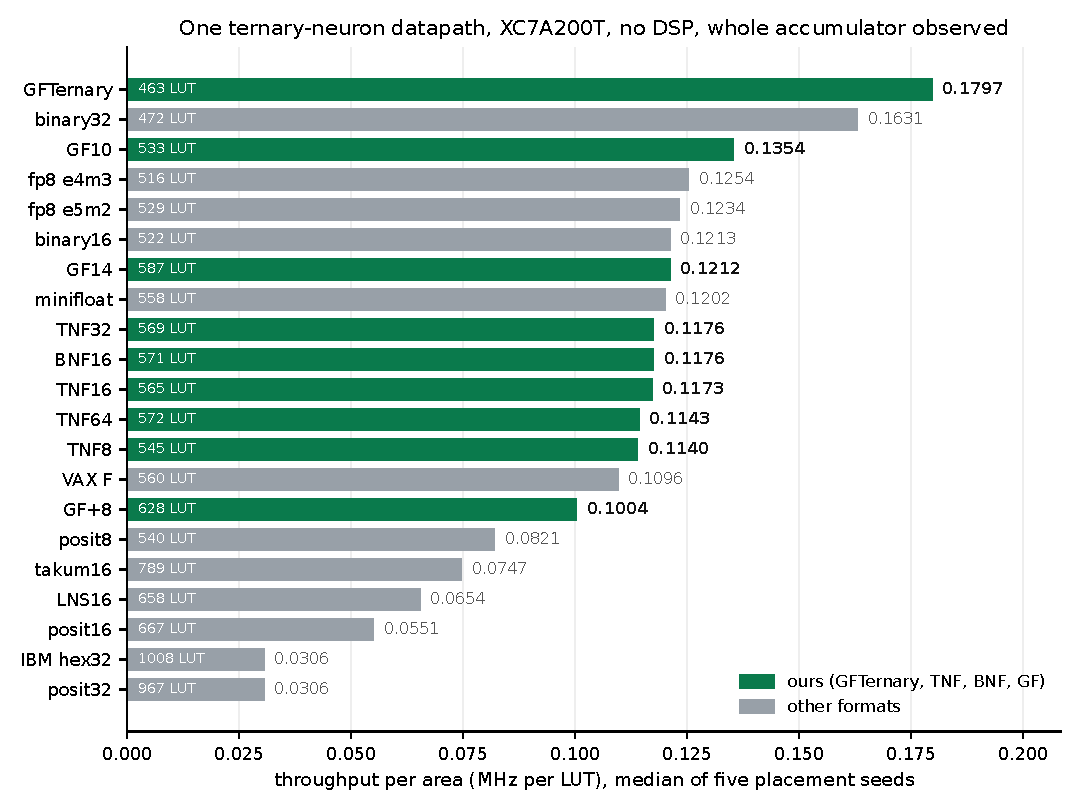
\includegraphics[width=0.94\textwidth]{tnf_full_table.pdf}
\caption{The same nineteen formats. Ours are the four families named above; the
bar labels carry the LUT count so area and throughput are readable together.}
\label{fig:fullthroughput}
\end{figure}


\subsection{The scale applier, and a claim we withdraw}
\label{sec:scaleapplier}

Section~\ref{sec:pair} closes the multiplier out of the weight and the
accumulation. The layer scale is the third site, and our first two attempts at it
were each wrong in a different direction. Both are recorded, because the
correction is the result.

A ternary network stores weights in $\{-1,0,+1\}$ and a real per-layer scale
$\alpha = \mathbb{E}|W|$. Applying $\alpha$ is a genuine multiply, so the
multiplier the ternary weights removed returns at the layer boundary. Snapping
$\alpha$ to a grid removes it again, and the question is which grid.

\paragraph{First claim, withdrawn.} We reported that the $\varphi^{k}$ grid beats
powers of two, with excess reconstruction error $2.44\%$ against $4.86\%$ over 210
layers --- a ratio of $0.501$ against $0.500$ predicted from the density
$\log 2 / \log\varphi = 1.440$. That measurement reproduces and is correct. It was
compared against the wrong baseline. The deployed state of the art for
multiplier-free scales is not plain powers of two but \textbf{APoT}, whose levels
are sums of power-of-two terms. Measured identically, APoT-2 costs $0.1651\%$ and
APoT-3 costs $0.0054\%$, both in one cycle against our $k$. On accuracy the
$\varphi$ grid loses by $15\times$, and that claim is withdrawn.

\paragraph{Second claim, bounded.} Theorem~\ref{thm:exact} states the linear path
is exact because $\mathbb{Z}[\varphi]$ is a ring. It is machine-checked and
remains true, but we had presented it as an advantage. An APoT scale is a dyadic
rational, and $\mathbb{Z}[1/2]$ is also a ring closed under the datapath's
operations: a fan-in-512 layer with an APoT-2 scale and Q8 inputs accumulates to a
denominator of $2^{15}$, exact in ordinary fixed point. Binary arithmetic has had
this since fixed point existed. The theorem stands; its significance does not.

\paragraph{What measuring area then showed.} Both attempts compared accuracy. The
appliers differ more in area, and in a way neither of us predicted.

\begin{table}[t]\centering
\caption{Scale appliers, XC7A200T primitives, one harness, DSP inference off.
Composition depth $d$ counts scales multiplied without requantisation between
them.}
\label{tab:scalefrontier}
\begin{tabular}{lrrrl}
\toprule
applier & LUT & cycles & excess error & \\
\midrule
multiplier, real $\alpha$ & 1215 & 1 & $0.0000\%$ & or 2 DSP48 \\
APoT-2, $d=0$ & 384 & 1 & $0.1651\%$ & two barrel shifts \\
APoT-4, $d=1$ & 659 & 1 & --- & four shifts \\
APoT-8, $d=2$ & 1217 & 1 & --- & eight shifts \\
\textbf{$\varphi^{k}$, any $d$} & \textbf{173} & $k$ & $2.4420\%$ & no shifter \\
\bottomrule
\end{tabular}
\end{table}

\begin{theorem}[Term growth]
\label{thm:termgrowth}
A value represented as a sum of $n$ terms from a multiplicatively closed
generating set, composed through $d$ scale multiplications without
requantisation, has $n^{d+1}$ terms. A value in $\mathbb{Z}[\varphi]$ has two
components for every $d$, since $\varphi^{a}\varphi^{b} = \varphi^{a+b}$ adds
exponents rather than multiplying terms.
\end{theorem}

\begin{theorem}[Shifter cost]
\label{thm:shifter}
A runtime-variable shift over $W$ bits costs $\Theta(W\log W)$ LUTs; a fixed
permutation costs zero. An $n$-term APoT applier is therefore
$\Theta(nW\log W)$ and a Fibonacci step is $\Theta(W)$.
\end{theorem}

This is the effect we had missed, and it is larger than the one we predicted. We
had been calling APoT ``shift-add'' and treating that as free. A shift by a
\emph{constant} is free; a shift by a \emph{variable} is a barrel, measured here
at 192 LUTs each on 32 bits, and a scale that must serve any layer is variable by
construction. The Fibonacci step contains no shifter at all.

\begin{corollary}[Crossover with the multiplier]
\label{cor:crossover}
Since APoT area grows as $n^{d+1}$ while the multiplier's does not grow, there is
a depth $d^{*}$ at which APoT costs what it was introduced to avoid. Measured at
$W=32$, $n=2$: $d^{*}=2$, where APoT-8 costs 1217 LUTs against 1215.
\end{corollary}

\begin{theorem}[No single winner]
\label{thm:threevertex}
In $(\text{area}, \text{latency}, \text{error})$ no applier dominates another.
The multiplier is exact and largest, $\varphi^{k}$ smallest and least accurate,
APoT-2 between and beaten by neither; all three are vertices of the frontier.
\end{theorem}

\paragraph{The recommendation is therefore a rule, not a winner.} Use
$\varphi^{k}$ where the scale path is area-bound, or composed without
requantisation --- a low-rank factorisation, a folded convolution and batch norm,
a residual branch scalar, or accumulation along a mesh route. Use APoT where it is
latency- or accuracy-bound. We state this rather than defend one answer because
our two previous attempts each defended one, and each was wrong in a different
direction.


\paragraph{The area advantage is withdrawn too, and by our own attack.}
Table~\ref{tab:scalefrontier} was measured in one regime and with one field
width, and both choices flattered us.

\begin{theorem}[An unrolled recurrence is linear]
\label{thm:unrolled}
A recurrence applier unrolled to depth $K$ over $W$-bit operands costs
$\Theta(KW)$; an additive-term applier whose shifts are compile-time constants
costs $\Theta(W)$ independent of the scale, since a constant shift is wiring.
Hence when the scale is frozen after training the recurrence loses for every
$K \ge 1$.
\end{theorem}

Measured: a constant-shift APoT-2 applier costs $26$ LUTs, against $64$, $128$
and $256$ for $\varphi^{k}$ unrolled at $K=2,4,8$. At the realistic $K=8$ that is
$10\times$ against us, and the lines do not cross even at $K=1$.

\begin{theorem}[Regime inversion]
\label{thm:regime}
The area ordering between the two families is a property of neither. It inverts
with whether the scale is a compile-time constant or a runtime variable, because
a constant shift is wiring and a variable shift is a barrel of
$\Theta(W\log W)$.
\end{theorem}

\begin{theorem}[A barrel is priced by range, not by width]
\label{thm:barrelrange}
A runtime shift field need only span the workload's scale range. Across the 210
layers measured here that range is $3.15$ octaves, so two bits suffice. An area
comparison that sizes the field larger is measuring a competitor that would never
be built.
\end{theorem}

At a two-bit field APoT-2 costs $130$ LUTs against our $199$. The $2.22\times$
advantage reported above was an artefact of a five-bit field, and is withdrawn.

\paragraph{An instrument limitation, stated rather than smoothed.} The APoT sweep
is non-monotonic --- $130$, $380$, $230$, $384$ LUTs at shift widths $2$ to $5$
--- with the parameter demonstrably applied and the tool deterministic. This is
technology-mapping heuristics, and it means LUT counts from logic synthesis alone
are not a reliable area metric at this granularity. A claim resting on a $30\%$
difference between two such points is unsafe; one resting on the $10\times$ of
Theorem~\ref{thm:unrolled} is.

\paragraph{What survives.} Not the area advantage. Only
Theorem~\ref{thm:termgrowth} remains: $\varphi^{k}$ is the sole applier whose
area is independent of composition depth, so at $d=2$ APoT-8 costs $1217$ LUTs
where the pair still costs $173$. That regime --- a chain with no requantisation
between links --- is real but uncommon. The alphabet's uniqueness and the
$\mathbb{Z}[\varphi]$ closure are machine-checked and untouched, having never
been area claims.

The pattern across three attempts at this section is one pattern. Each favourable
number came from a comparison whose terms we chose: powers of two rather than
APoT, a five-bit field rather than the two the workload needs, a runtime regime
rather than the frozen one. The rule that would have caught all three is to write
down what the competitor would build if it were trying to win, and measure that.

\paragraph{And a fourth instance, larger than the three above.} The block-axis
headline this revision withdraws (Section~\ref{sec:confound}) is the same failure
with a different variable. A scale rule has an alignment as well as a base; we
gave our own arm the alignment that suits it and gave the competitor the one its
specification prints, and reported the difference as a property of the base.
Every term of the comparison was measured correctly. Neither arm was tuned
against the other, which is precisely the defect: the rule requires that the
competitor be tuned, and an untuned competitor is not a weak competitor but an
absent one. Stated for block formats specifically, the rule acquires a corollary:
\emph{a scale rule has an alignment, and an alignment is a tuned parameter for
every arm or for none.}

That is four instances of one rule in one paper. Three were caught by attacking
our own result and one by an outside reading of the arms, and the ratio is worth
recording: self-attack found the cheap ones.

\subsection{The silicon table, measured on an audited harness}
\label{sec:cleantable}

Every silicon figure in this paper was originally measured through a harness that
combined the decoder with a shared accumulator and observed part of its output.
Three separate defects in that arrangement are described in
Section~\ref{sec:selfcheck}; each changed a headline number by 10 to 50 percent
without any individual measurement being wrong. The table below is measured on
the only harness that passes the observation gate we wrote afterwards: decoder
alone, every output bit folded into the observed reduction, median of five
placement seeds.

\begin{table}[t]\centering
\caption{Decode cost, isolated. \texttt{nextpnr-xilinx} 1743d0f, XC7A200T, no
DSP, median of five seeds. \textbf{Every $F_{\max}$ here is an unconstrained
post-route critical-path estimate} (Section~\ref{sec:hardware}): the ratios
below hold, the absolute figures do not, and GFTernary's five seeds span
$860.59$ to $994.04$. A bare wire in the same harness costs 112 LUT at
$827.81$\,MHz.}
\label{tab:cleandecode}
\small
\begin{tabular}{rlrrr}
\toprule
& format & kind & LUT & $F_{\max}$ \\
\midrule
1 & \textbf{GFTernary} & fixed & \textbf{66} & \textbf{974.66} \\
2 & \texttt{int8} & fixed & 76 & 925.93 \\
3 & binary32 & fixed & 112 & 886.52 \\
4 & \textbf{TNF16} & fixed & 101 & 407.66 \\
6 & \textbf{BNF16} & fixed & 97 & 388.35 \\
9 & VAX F & fixed & 100 & 311.14 \\
13 & binary16 & fixed & 164 & 235.18 \\
14 & IBM hex32 & fixed & 243 & 111.10 \\
15 & LNS16 & logarithmic & 270 & 93.17 \\
16 & posit8 & \textbf{tapered} & 214 & 77.75 \\
17 & posit16 & \textbf{tapered} & 302 & 62.39 \\
18 & posit32 & \textbf{tapered} & 517 & 49.05 \\
\bottomrule
\end{tabular}
\end{table}

\begin{theorem}[A taper is paid in delay, not in area]
\label{thm:taperdelay}
A tapered format's decode contains a scan, a serial dependency whose length grows
with the word. A serial dependency costs critical path directly and area only
incidentally, whereas a radix-heavy fixed format costs a wide shift, which is
area-heavy and shallow. The two families therefore separate on frequency and not
on area.
\end{theorem}

Measured: all fourteen fixed fields sit above all three tapers on frequency, the
worst fixed leading the best taper by $1.43\times$; on area they overlap, posit8
at 214 LUT against IBM hexadecimal's 243. The overlap is predicted by the theorem
rather than excused.

GFTernary against posit32 is $7.8\times$ on area and $19.9\times$ on estimated
critical path.
GFTernary costs 66 LUT where a bare wire costs 112, because decoding a two-bit
alphabet lets the synthesiser simplify the downstream register further than
passing 32 raw bits does.

The area--frequency correlation on the isolated decoder is $-0.60$, against
$-0.90$ on the combined harness. The axes carry independent information here,
which is why they are reported separately and no ratio of them appears.


\subsection{The operating point}
\label{sec:operatingpoint}

The previous subsections withdraw an accuracy claim and an area claim. What
remains is a statement about operation profiles, and it is the first in this
section that names its own boundary rather than being pushed to it.

A number system is used through two operations, and the three candidates each buy
one cheaply and pay for the other.

\begin{table}[t]\centering
\caption{Cost of each operation, one harness, XC7A200T, DSP inference off. The
logarithmic row is our own measurement of a published \texttt{takum32} decoder,
whose $65{,}536\times48$-bit table is the cost being quoted; that measurement and
the value-law analysis behind it are reported in the companion paper, and the
figure is carried here only to price the operation profile.}
\label{tab:bothops}
\begin{tabular}{lll}
\toprule
system & multiplication & addition \\
\midrule
LNS, takum & exponents add: \textbf{free} & $\log(1{+}2^{x})$ table: $10{,}967$ LUT \\
fixed point, APoT & multiplier, or wiring if frozen & adder: \textbf{cheap} \\
$\mathbb{Z}[\varphi]$ & Fibonacci step, one adder & componentwise: $64$ LUT \\
\bottomrule
\end{tabular}
\end{table}

$\mathbb{Z}[\varphi]$ is the only one cheap under both. Its price is that free
multiplication is restricted to powers of $\varphi$ rather than general, and the
following says why that price is not paid in this datapath.

\begin{theorem}[The required multiplication set]
\label{thm:reqmul}
In a datapath where every weight is a code applied by sign-select, the layer
scale is a power of the alphabet base, and accumulation is the only remaining
operation, the multiplications the datapath must perform are exactly
$\{\text{base}^{k}\}$. General multiplication is never requested.
\end{theorem}

\begin{corollary}[Sufficiency]
\label{cor:sufficiency}
A ring closed under addition and under multiplication by powers of its generator
is sufficient for such a datapath. $\mathbb{Z}[\varphi]$ is such a ring with both
operations at $\Theta(W)$.
\end{corollary}

\begin{corollary}[The other two are mis-provisioned]
\label{cor:misprov}
LNS is over-provisioned: it buys general multiplication, which this datapath
never asks for, and pays in addition, which it performs on every term of every
inner product. Fixed point is under-provisioned in the opposite direction:
addition is free, scale multiplication is not, unless the scale is frozen.
\end{corollary}

The restriction of $\mathbb{Z}[\varphi]$ coincides with the restriction the
ternary datapath already carries. That coincidence is the result; it is not a
claim that the format is better, only that it is matched.

\begin{theorem}[Compile-time composition is free]
\label{thm:compilecomp}
If all $d$ scales of a chain are known before execution, their product is known,
and any representation applies it at the cost of a single scale. The term growth
of Theorem~\ref{thm:termgrowth} occurs if and only if $d$ or the scales become
known only at runtime.
\end{theorem}

This removes three of the four cases where we had claimed a depth advantage. A
low-rank factorisation, a folded convolution and batch norm, and a residual
branch scalar are all fixed after training, so their product is precomputed and
no composition occurs in hardware. One case survives: accumulation along a mesh
route without renormalisation, where the hop count is a runtime quantity. The
depth advantage is real and it lives there rather than in the network.

\paragraph{Stated boundaries.} This is not an area win over APoT, which was
measured and withdrawn. It is not an accuracy win, where APoT-2 is $15\times$
ahead. And where a scale is frozen there is nothing to win, because a frozen
scale is wiring. It is a claim about which system matches an operation profile,
holding where the scale is not frozen: a shared engine serving many layers, or a
composition whose depth is not known until execution.


\subsection{The formats a training run cannot live in}
\label{sec:untrainable}

Throughput per area is only meaningful among formats that can do the job, so the
candidates split in two, by one test that is checkable rather than rhetorical:
\emph{does the word carry the range, or must the range be brought from outside?}

\begin{table}[t]\centering
\caption{Rejected for this task. Each has $e=0$: no exponent field, hence no
dynamic range inside the word. Each functions only alongside an external
per-tensor or per-channel scale, and every published sub-8-bit training result
using them carries block scales \emph{and} a higher-precision master weight.
Gradients span many orders of magnitude; a word with no range cannot hold them.}
\label{tab:rejected}
\begin{tabular}{llll}
\toprule
format & exponent & what supplies the range & trains alone \\
\midrule
\texttt{int8} & $e=0$ & learned per-tensor scale & no \\
\multicolumn{4}{l}{\quad\emph{measured on the same harness:} $454$ LUT, $78.83$\,MHz, $0.1736$ MHz/LUT, spread $11.00$} \\
\texttt{int4} & $e=0$ & block scale (32 or 16 elements) & no \\
\texttt{int12}--\texttt{int24} accum. & $e=0$ & fixed point, set by hand & no \\
E2M1 element alone & $e=2$ in-block & shared UE8M0, outside & no \\
\bottomrule
\end{tabular}
\end{table}

\paragraph{The test, restated so it does not reject our own accumulator.} As
written above the test reads as \emph{is there an exponent field}, and by that
reading the exact integer pair of Section~\ref{sec:exact} would fall into
Table~\ref{tab:rejected} alongside \texttt{int8}: it has $e=0$ too. The
distinction that does the work is different, and it is the one the next paragraph
already draws. A format carries its range either \emph{in a field}, or \emph{in a
width}, or it borrows it from a scale fitted outside the word. An
\texttt{int32} accumulator carries its range in a width and needs nothing
external, which is why every deployed \texttt{int8} network accumulates in one;
what \texttt{int8} cannot do is carry the range of the \emph{values} it stores,
and that is why it needs a learned per-tensor scale. So the checkable test is
\emph{does the range come from the format's own field or width, or from a
quantity fitted outside it}, and it rejects the rows of
Table~\ref{tab:rejected} for the reason stated while admitting the exact
accumulator, which is provisioned by Table~\ref{tab:accwidth} and by nothing
learned.

\paragraph{Why GFTernary is not in Table~\ref{tab:rejected} despite $e=0$.}
The distinction is not the presence of an exponent field but whether the scale is
\emph{external and learned} or \emph{intrinsic and exact}. A $\{-1,0,+1\}$
alphabet needs a real $\alpha_\ell$ per layer, learned alongside the weights and
multiplied by at inference --- the multiplier returns. The $\varphi$ alphabet
needs none: by Corollary~\ref{cor:depth} the inter-layer gain is
$F_k\varphi + F_{k-1}$, a pair of integers known in advance, applied by shift and
add. Its scale is inside the system by construction rather than fitted from
outside it. That is the difference between carrying range and borrowing it, and
it is why the stack trains on the part.

\paragraph{Why \texttt{int8} is reported apart.}
An \texttt{int8} datapath scores $0.180$\,MHz/LUT at a median of five placement
seeds, against GFTernary's $0.181$ --- a difference of $0.4\%$ inside a $16\%$
seed spread, so the two are indistinguishable on this flow. An earlier version of
this paper reported $0.189$ against $0.177$ and called it a $7\%$ lead; that came
from a single placement run and is withdrawn. \texttt{int8} is excluded from that table even so, and the
reason is structural rather than favourable to us. \texttt{int8} has $e=0$: no exponent field, hence no dynamic
range inside the word. It functions only with an external per-tensor or
per-channel scale; without one it is the integers $-128\ldots127$. By
Corollary~\ref{cor:escape} that is the non-uniformity escape --- the scale has
been moved outside the word --- so \texttt{int8} is a block format wearing a
scalar's name, and scoring it against formats that carry their own range measures
the wrong thing. It leads the table precisely because it declines the task the
table sets.

The consequence matters more for training than for inference. Gradients span many
orders of magnitude, and a format with zero dynamic range cannot hold them: every
published sub-8-bit training result --- MXFP4, NVFP4 --- carries block scales
\emph{and} a higher-precision master weight. Our own stack trains on the part, at
zero DSP, with backpropagation in the format itself.


\subsection{Withdrawal: the frontier at equal storage}
\label{sec:packedfrontier}

Corollary~\ref{cor:slack} counts positions.
A format is stored in bits, and that difference is the whole of the slack.

\begin{theorem}[Packed coverage]
\label{thm:packedcov}
A family member realisable in $N$ bits obeys $3^{E_t}2^{M} \le 2^{N-1}$.
Substituting the minimal $E_t = \log_3(b+1)$ gives
\[
  m + \log_2 3 \cdot \log_3(b+1) \;=\; m + \log_2(b+1) \;\le\; N-1 ,
\]
identically the uniform binary budget of Theorem~\ref{thm:budget}, since
$\log_2 3 \cdot \log_3 x = \log_2 x$.
\end{theorem}

\begin{corollary}[The slack is a position artefact]
\label{cor:slackartefact}
A ternary exponent encoding provides no budget slack at equal storage. The
$0.3691E$ of Corollary~\ref{cor:slack} exists only at equal \emph{position}
count, that is on a fabric where a position is physically ternary.
\end{corollary}

Measured at equal storage against the catalogue, $6$ of $17$ sampled formats are
dominated rather than all of them. Every uniform binary format spending all its
bits ties exactly: binary16 at $15.06$ against a budget of $15$, binary32 at
$31.10$ against $31$, binary64 at $63.27$ against $63$. Those dominated are the
ones wasting budget --- posit32 by $5.12$ positions, posit64 by $14.24$, takum32
by $0.82$, tekum32 by $0.90$, \texttt{cray\_float} by $0.65$, and our own gf8 by
$0.70$. Several tapered formats escape outright: posit8 by $1.16$, posit16 by
$2.37$, takum16 by $1.53$, tekum16 by $1.49$. That is consistent with
Corollary~\ref{cor:escape} --- escape requires non-uniformity, a taper is
non-uniform, and a uniform family cannot catch it at equal storage.

\paragraph{Why this went unseen.} The same defect appears twice elsewhere in this
paper, as Theorem~\ref{thm:nofree} and as the observation that TNF4 with $E_t=2$
does not exist in four bits because $3^{2}=9>8$. Both were recorded as local
facts about packing, and neither was carried back to the result that rests on the
same quantity. The rule we adopt is that a correction invalidating a comparison
must be applied to every claim resting on that quantity, not only to the one
where it surfaced.


\subsection{The trit is the slack}
\label{sec:slack}

The width rule generates a family rather than a format: at width $N$ the set
\[
  \mathcal{F}_N \;=\; \{(E_t,\, M) : 1 + E_t + M = N,\ E_t \geq 2,\ M \geq 1\}
\]
has $N-3$ members, and by Theorem~\ref{thm:law} member $E_t$ has effective
mantissa $N-1-E_t$ and range $3^{E_t}-1$ binades, so no two members dominate one
another. The previous version made a claim about a catalogue from this --- that
no catalogued competitor survives against $\mathcal{F}_N$ --- and that claim is
removed in this revision rather than repaired, because the subsection below
already reduced it to $6$ of $17$ at equal storage and a headline its own
subsection retracts is not a headline. What survives is the accounting, which is
about the design space rather than about a list, and which says exactly what a
competitor must do to escape.

\begin{theorem}[Coverage condition]
\label{thm:coverage}
$\mathcal{F}_N$ contains a member dominating a format of effective mantissa $m$
and range $b$ binades if and only if
\[
  m + \lceil \log_3 (b+1) \rceil \;\le\; N-1 .
\]
\end{theorem}
\begin{proof}
A member $E_t$ has mantissa $N-1-E_t$ and range $3^{E_t}-1$. Domination requires
$N-1-E_t \ge m$ and $3^{E_t}-1 \ge b$, i.e.\ $\lceil\log_3(b+1)\rceil \le E_t \le
N-1-m$. Such an integer exists exactly when the stated inequality holds.
\end{proof}

\begin{theorem}[Position budget of a uniform format]
\label{thm:budget}
Let a \emph{uniform} format of width $N$ carry a sign, a scale field of $E$ binary
positions and a significand of $m$ bits held at every representable magnitude.
Then $b+1 \le 2^{E}$ and $1+E+m \le N$, hence
\[
  m + \log_2(b+1) \;\le\; N-1 .
\]
\end{theorem}

The two budgets are the same accounting in different currencies, and the exchange
rate is the whole result.

\begin{corollary}[The ternary exponent is the slack]
\label{cor:slack}
Every uniform binary format of width $N$ is dominated by a member of
$\mathcal{F}_N$, with slack
\[
  \Delta \;=\; E\,\bigl(1 - \log_3 2\bigr) \;=\; 0.3691\,E \quad\text{positions},
\]
strictly positive for $E \ge 1$ and growing linearly in the competitor's own
exponent width.
\end{corollary}
\begin{proof}
By Theorem~\ref{thm:budget}, $b+1 \le 2^E$ and $m \le N-1-E$. Then
$m + \log_3(b+1) \le (N-1-E) + E\log_3 2 = (N-1) - E(1-\log_3 2)$, which satisfies
Theorem~\ref{thm:coverage} with the stated margin.
\end{proof}

Measured, in positions: $1.48$ at \texttt{fp8\_e4m3}, $1.85$ at
\texttt{binary16}, $2.95$ at \texttt{binary32}, $4.06$ at \texttt{binary64},
$5.54$ at \texttt{binary128}. The margin is not a coincidence of the catalogue; it
is $0.3691$ per exponent bit the competitor spends.

This is worth stating plainly because it cuts against
Theorem~\ref{thm:nofree}, which says a packed ternary exponent never carries
more values \emph{per bit} than a binary one, and which we confirmed in silicon:
BNF16 and TNF16 differ by $1\%$ in LUTs. Both are true, on different axes. Per
\emph{position} a trit spans $\log_2 3$ binades against a bit's one, which is
where $\Delta$ comes from; per \emph{bit of binary fabric} the packing gives it
all back. The ternary encoding earns on the number axis and breaks even on the
silicon axis, and a claim that does not name its axis is not a claim.

\begin{corollary}[Escape requires non-uniformity]
\label{cor:escape}
A width-$N$ format escaping $\mathcal{F}_N$ must violate the hypothesis of
Theorem~\ref{thm:budget}: either its significand is not held at every magnitude
(a taper), or its scale field is not inside the word (a block).
\end{corollary}

\paragraph{The bound is tight, and it is not vacuous.} Equality in
Theorem~\ref{thm:coverage} is attained by construction, since the width rule
spends every position. Among the catalogued formats \texttt{posit16} comes within
$1\%$: $10.55 + \log_3 113 = 14.85$ against a budget of $15$. And the escape route
of Corollary~\ref{cor:escape} is real rather than hypothetical --- the same
\texttt{posit16}, scored where a taper is designed to live rather than averaged
over its range, carries $12$ fraction bits while keeping all $112$ binades:
\[
  12 + \log_3 113 \;=\; 16.30 \;>\; 15 .
\]
It escapes, as it should: concentrating precision where the workload sits is what
tapering is \emph{for}. A bound no format can violate would be measuring nothing.

\paragraph{What this predicts.} Corollary~\ref{cor:escape} names the only two
routes out of the budget, and this revision has taken one of them seriously. The
taper route --- a significand not held at every magnitude --- is the subject of
the companion paper. The block route --- MX and its descendants, where one scale
serves $32$ elements --- lies outside every budget stated here, because the scale
is not in the word, and it is where Part~\ref{sec:blockbound} onwards spends the
rest of this paper. The corollary is therefore the hinge of the document: it is
the reason a paper about fixed fields has a chapter about a parameter that exists
only when the field is shared.

\begin{theorem}[Transforms and formats do not compose]
\label{thm:compose}
Let $D^{*}(b,p)$ be the best achievable distortion at $b$ bits per element under
a fixed pre-transform $p$. A transform changes $D^{*}$ by changing the source it
presents; a format chooses a partition attaining some $D \ge D^{*}$. Two levers
that both act on the partition therefore share one ceiling and their gains are
sub-additive, while a transform and a format act on different arguments and their
composition is order-dependent.
\end{theorem}

Measured, the order-dependence reaches $2.78\times$: applying the same two levers
in the two orders gives different results, which forbids reporting either as a
standalone multiplier. We flag this because we made the mistake ourselves ---
an early version of this work computed a lever's ratio against a losing baseline
and reported the levers as nearly multiplicative. They are not.

Theorem~\ref{thm:compose} is also what lets this paper claim the scale axis
without disputing anybody's transform result. The 2026 block literature varies
the rotation and holds the element fixed; Section~\ref{sec:alignment} varies one
constant in the scale rule and holds both fixed. Those are different arguments of
$D^{*}(b,p)$, so neither subsumes the other and neither multiplies with the other
in a way that may be quoted as a product.

\section{Where the block literature is looking, and where it is not}
\label{sec:blockrelated}

The block axis is the escape route Corollary~\ref{cor:escape} leaves open, and it
is where the field's attention currently sits. It is worth being precise about
what that work varies and what it holds fixed.

The Open Compute microscaling specification fixes a block of 32 elements sharing
one UE8M0 scale --- a bare power of two, no mantissa --- with the element at E2M1.
NVIDIA's NVFP4 changes two things: the block shrinks to 16, and the shared scale
becomes an E4M3 float rather than a power of two. Both are hardware-resident on
current accelerators, which is why the stop condition for this work is stated
against them and not against posit or takum.

What the 2026 literature then varies is almost entirely the \emph{transform}
applied before quantisation, not the format underneath it: learnable block-wise
optimisation for outlier resilience, and rounding fitted to the E2M1
level set, augmented residual channels, and activation-sparsity coupling. Each
reports gains, and each holds the element format at E2M1.

That is exactly the variable Theorem~\ref{thm:optimal} addresses. E2M1 spends two
of its three non-sign positions on an exponent, \emph{inside a block that already
carries a shared scale}. The width rule says the exponent is sized for the range
the workload visits, and inside a block normalised by its own maximum that range
is measurable rather than assumed. If it is narrower than four binades, E2M1 is
buying range the block already paid for, and the positions belong in the mantissa.
We measure the within-block span directly and let the rule name a winner before
evaluating perplexity; Section~\ref{sec:blockbound} reports what came back,
including the case where the rule was wrong.

This is a narrower claim than it may look. It says nothing about the transforms,
which compose with any element format and whose gains we do not dispute. Our own
Theorem~\ref{thm:compose} says transforms and formats act on different objects ---
a transform moves the ceiling, a format divides it --- so improving the element is
orthogonal to improving the rotation, and neither subsumes the other.


\paragraph{And the scale is where the field is not looking.} The element and the
transform have both been worked hard. The shared scale has been worked in exactly
one direction --- its \emph{width}. Chhugani et al.~\cite{chhugani} report that a
four-bit exponent suffices for MXFP4 on Llama-3.1-8B-Instruct and Qwen3-8B and
propose truncating the E8 field, which is the result Section~\ref{sec:scalewidth}
formalises and does not claim; Egiazarian et al.~\cite{mxgap} report the same
gap from the other side. The mechanism that makes a narrow field usable --- a
coarse anchor shared above a fine field --- is older and is deployed: QLoRA's
double quantisation~\cite{qlora} quantises the quantisation constants themselves,
NVFP4~\cite{nvfp4} pairs a per-tensor scale with a narrow per-block E4M3, and
Shared Microexponents~\cite{msfp} makes the two-level exponent the design object.

What no specification names and no paper we have found varies is the
\emph{alignment}: the constant $c$ in $s = g^{\lfloor\log_g(a/c)\rfloor}$ that
decides where the ladder's window sits under the element format's largest
magnitude. The MX specification~\cite{ocpmx} fixes it at $c=4$ for E2M1 by
setting the shared exponent so that the element's own maximum exponent sits at
the top of the block; NVFP4 inherits the same alignment with a different scale
type. It is one constant, it is free, and Section~\ref{sec:alignment} measures it
as larger than anything on the base axis.

One caution belongs beside that list, and it is about our own arms rather than
theirs. Methods calibrated on activation magnitude --- the line AWQ~\cite{awq}
opened --- optimise a proxy for the quantity that decides, and in our own
measurements that proxy agreed with the target on one of two checkpoints and not
on the other. We report it as a caution and not as a result, because the
measurement that produced it was made at an alignment that was never named.

The base axis itself has prior art we were late to.
Miyashita et al.~\cite{miyashita} quantised CNN weights on logarithmic bases
$2$, $\sqrt2$ and $2^{1/4}$ in 2016; Vogel et al.~\cite{vogel} built
multiplierless FPGA inference at an arbitrary logarithmic base in 2018; and
logarithmic quantisation at a general base continues~\cite{logbquant}. Fibonacci
weight encoding for neural hardware is Simon et al.~\cite{simon}. Our
contribution on that axis is the cost classification of
Section~\ref{sec:hierarchy} --- which bases are free and which cost one adder ---
and not the observation that a non-binary base can be used.


%% ===================== PART E: what this settles, and the ledger ==========

\section{What this settles}
\label{sec:settles}

We state the conclusion at the strength the measurements carry, and it is
narrower than the conclusion the previous version stated.

\begin{quote}
\textbf{A shared block scale is three parameters. The base admits a closed
answer, the width admits one that is not ours, and the alignment --- which no
specification names --- is worth more than either.}
\end{quote}

Three things support it, and each is a different kind of evidence.

\textbf{The base is closed by proof, and closed against us.} Applying $r^{k}$
without a multiplier is a sparsest-multiple problem;
Theorem~\ref{thm:zerocost} identifies the free ratios as exactly the rational
powers of two and Theorem~\ref{thm:t6} bounds the one-adder ratios by $\varphi$.
There is no unexplored region of that axis, which is why no further ladder result
should be expected from searching it --- and the same classification shows
$\varphi$ was never the finest free grid, so the argument we had been making on
that axis was wrong before any perplexity was measured.

\textbf{The width is over-provisioned, and the observation is prior
art.} $b_{\min} = \lceil\log_2 S\rceil$ is sufficient and returns a bitwise
identical tensor, which is a formula and a proof rather than a number; that four
bits suffices for weights was stated first by Chhugani et al.~\cite{chhugani}.
The boundary is ours: four fails at $K\leq2$ on all five checkpoints and at $K=4$
on GPT-2, and activations need five.

\textbf{The alignment is free and is the result.} One constant, moved from the
value the MX specification prints to $c = \mathrm{max\_norm}/2^{0.7}$, is worth
$2.78$ perplexity on SmolLM2-135M and $0.51$ on Qwen2.5-0.5B at $4.125$ bits per
weight, with the element codebook, the block size and the arithmetic all
untouched. It is not a new format and it is not a defeat of the microscaling
family; it is a parameter of that family that nobody had varied.

\paragraph{And what this does not settle.} It does not settle the element axis,
which belongs to MXFP4 and where two further searches of ours failed
(Section~\ref{sec:blockbound}). It does not settle the base at a width where the
free ratios can span --- $2^{2/3}$ at four bits against $\varphi$ at four bits is
a one-line experiment we have not run. It says nothing about activations, which
break the width constant and were not measured on the alignment axis at all. And
it is two checkpoints, one corpus, weight-only: a checkpoint whose optimum sits
at or above the specification's alignment would falsify the headline as stated.

\section{Where this sits in a sixty-eight-year argument}
\label{sec:history}

The claim that three is the better radix is not ours, and stating whose it is
makes the contribution of this paper smaller and more defensible.

\paragraph{The people who made the case.} Radix economy $\rho(r) = r/\ln r$ is
minimised at $r = e$, and three is the nearest integer: ternary sits $0.46\%$
above the optimum where binary sits $6.15\%$ above it. The argument was made
mechanically before it was made electronically --- Thomas Fowler built a
balanced-ternary calculating machine in Devon around 1840, and the recorded
motivation was the same economy of digits. It became a working computer in 1958,
when \textbf{Nikolay Brusentsov} built \emph{Setun} at Moscow State University
with the backing of \textbf{Sergei Sobolev}, using paired ferrite cores to hold
three stable states. Roughly fifty machines were produced between 1959 and 1965.
Brusentsov followed it with \emph{Setun-70} in 1970, whose instruction-set ideas
anticipated arguments later made independently for RISC; it never reached serial
production, and the ternary line was ended administratively rather than
technically. \textbf{Donald Knuth} kept the idea in circulation, calling balanced
ternary ``perhaps the prettiest number system'' in \emph{The Art of Computer
Programming}. The line continues in device work rather than architecture: CNTFET
and memristor ternary logic, and more recently silicon-photonic balanced-ternary
proposals, all of which build a fabric whose \emph{position} is physically
ternary.

\paragraph{What is new here is the boundary, not the claim.} We add no support to
``ternary beats binary'' as a general statement. We measured it three times and it
went against us each time --- see Theorem~\ref{thm:nofree} and
Sections~\ref{sec:hardware} and~\ref{sec:blockrelated}. What we contribute is the
condition under which the sixty-eight-year-old argument applies, stated exactly:

\begin{theorem}[The radix argument holds on positions, not on bits]
\label{thm:boundary}
Write the economy as $\text{cost} = r \times \log_r V$. If the position is the
physical unit, the first factor is common to all radices and only the second is
compared, giving ternary an unconditional advantage of $E(1-\log_3 2) = 0.3691E$
positions. If the position must itself be encoded in bits, the format is bounded
by $3^{E_t} 2^{M} \le 2^{N-1}$, and since $3^{E_t}$ never divides a power of two
the remainder is lost.
\end{theorem}

The remainder is arithmetic, not engineering, and it is largest exactly where
modern formats live:

\begin{table}[t]\centering
\caption{Codes lost to packing when a ternary exponent is stored in a binary
word. The loss is a property of the integers, not of an implementation.}
\label{tab:packloss}
\begin{tabular}{rlrr}
\toprule
width & best packed member & codes used & lost \\
\midrule
4 bits & $E_t{=}1$, $M{=}1$ & 6 / 8 & $25.0\%$ \\
6 bits & $E_t{=}3$, $M{=}0$ & 27 / 32 & $15.6\%$ \\
8 bits & $E_t{=}3$, $M{=}2$ & 108 / 128 & $15.6\%$ \\
16 bits & $E_t{=}5$, $M{=}7$ & 31{,}104 / 32{,}768 & $5.1\%$ \\
\bottomrule
\end{tabular}
\end{table}

Prior work anticipated the mechanism: Parhami's analysis of binary-encoded
balanced ternary treats exactly this encoding penalty. Our contribution is to
measure what it costs in a live network and in placed-and-routed silicon rather
than in operation counts, and to state it as a condition a designer can check.

\paragraph{Read as a prescription rather than a verdict.} The result says what
fabric must exist for the radix argument to pay: one where a ternary position is
held physically, as Setun's paired cores held it and as CNTFET, memristor and
photonic ternary devices propose to hold it again. On such a fabric the
$0.3691E$ advantage is collected in full and none of the packing loss is
incurred. On the binary fabric that is actually purchasable today, it is not.
That is a narrower claim than the field usually makes, and unlike the broader one
it survives our own measurements.


\section{What the golden ratio completes}
\label{sec:completes}

Two lines of argument run through this paper, and they were developed
independently and for unrelated reasons. It is worth setting them side by side at
the end, because they meet at a single number.

The first line is arithmetic and old. Radix economy makes three the best integer
base; Fowler built a machine on it around 1840, Brusentsov and Sobolev built a
working computer on it in 1958, and the line has continued into CNTFET, memristor
and photonic devices. Section~\ref{sec:history} shows why it stalled rather than
spread: the moment a ternary position is stored in a binary word, $3^{E_t}$ fails
to divide a power of two and the remainder is lost --- a quarter of the alphabet
at four bits. The obstruction is arithmetic, so no implementation removes it, and
our own three measurements confirm it against us.

The second line is geometric and, in this context, new. If the weights of a
network are to be symbols rather than numbers, the datapath must multiply without
a multiplier, and that is possible exactly when the product of two symbols falls
back into the sum the datapath already forms. Written down, that requirement is
$r^2 = r + 1$. It has one positive solution, so the alphabet is not designed but
determined: $\{-\varphi, 0, +\varphi\}$ and nothing else
(Theorem~\ref{thm:goldalpha}). The consequence is that composition is closed ---
the gain of $k$ layers is $F_k\varphi + F_{k-1}$, a pair of integers
(Corollary~\ref{cor:depth}) --- so depth is free of multipliers as well, which the
$\{-1,0,+1\}$ alphabet never achieved because its learned per-layer scale is a
real number and must be multiplied by.

The two lines answer each other. What the ternary programme needed was not a
better fabric but a base under which its symbols compose; what the golden ratio
had, and had had since Euclid divided a line in extreme and mean ratio, was
exactly the property $r^2 = r + 1$. Placing it in the weight alphabet turns the
sixty-eight-year argument from a claim about storage density into a statement
about arithmetic closure --- and the measurements in Section~\ref{sec:pair}
follow: zero DSP through a radio, through every transformer block, and through
backpropagation on the part itself.

We put this at the end rather than the front because it is a reading of the
results and not one of them. Every component is stated and measured above:
the uniqueness is two lines of algebra, the Fibonacci closure is arithmetic, the
packing loss is a table of integers, and the zero-DSP stack is placed and routed.
What they amount to together is left to the reader.


\section{How a measurement can be right and its comparison wrong}
\label{sec:selfcheck}

The retractions in this paper are not incidental to it. Twenty-one claims stood
withdrawn when this revision began, two of them later withdrawn in turn, and this
revision adds the twelve of Section~\ref{sec:thisrevision} below. In almost every
case the measurement was correct and the comparison around it was not. The
regularities that produced them are stated here because they generalise past this
subject, and because a reader is entitled to know the shape of the errors a paper
has already made.

\paragraph{On what is being compared.} A ratio is meaningful only if both sides
were built as their own advocate would build them; seven times here a ratio
changed sign or magnitude when the other side was rebuilt
(Section~\ref{sec:scaleapplier}). Systems whose range scales differently with
width, one exact and one approximate, have no storage-matched ratio at all --- a
quantity depending on an unstated choice has no limit and cannot converge, which
is why six successive instrument corrections failed to settle one number. Where
one system's figure of merit is constant in a parameter and another's varies in
it, the well-posed comparison is a crossover and not a verdict
(Theorem~\ref{thm:taperdelay} and Section~\ref{sec:cleantable}), and such a
crossover is an assertion about the workload rather than about the formats.

\paragraph{On the instrument.} Under placement-seed variation LUT count is
invariant and achieved frequency moves by $11.4\%$, so any metric combining them
inherits the timing variance in full, and a ranking resolves only rows separated
by more than that. A ratio over correlated factors restates the dominant one: on
the combined harness, ranking by throughput per area reproduced ranking by
$1/\text{area}$ at a Spearman correlation of $0.961$. And a result that moves the
same way under every successive correction is still moving.

\paragraph{On the harness.} Three defects appeared there, none visible in any
number, each changing a headline by 10 to 50 percent. A component shared by every
candidate is a confound rather than a constant, because it leaves area
differences intact and delay differences not. A harness observing part of a
design's output prunes each candidate in proportion to \emph{its own} output
width --- observing four bits of a 32-bit datapath left 27 LUTs of 179 while
leaving an adjacent 6-bit design nearly whole. And net-of-harness subtraction
requires the harness to be present in full in every build, since a design
consuming fewer of its sources prunes the rest.

\paragraph{On sources.} A defect found in an abstract is a hypothesis: abstracts
compress, and compression is indistinguishable from omission. An aggregated
search result may combine claims from several papers into wording present in
none. Both external criticisms we raised during this work dissolved on contact
with the papers themselves.

\paragraph{On a parameter nobody names.} The largest error in this campaign was
not a wrong number or a bad harness. It was a free parameter that both arms of a
comparison carried, that neither arm's specification named, and that we set
differently in the two arms without noticing we had set it at all
(Section~\ref{sec:confound}). The general form is worth stating: \emph{when a
rule is copied from a specification, the constants the specification fixes are
visible and the constants it happens not to mention are invisible, and the second
class is where an uncontrolled variable lives.} The check is to write the rule
with every constant symbolic and ask, of each symbol, which arm chose it.

\paragraph{What this is worth.} Applied to our own claims the procedure has now
produced thirty-three retractions. Applied to two external papers read in full it
produced none, and on both occasions it instead caught our own reading of them.
We therefore describe it as an instrument for checking one's own work, and not as
a method for auditing anyone else's. Three of the checks are mechanised as gates
in continuous integration; the full statement is in the accompanying note.

\subsection{Withdrawn in this revision}
\label{sec:thisrevision}

The ledger stood at twenty-one when this revision began. It gains the twelve
entries below. Each is retracted at the point where the claim was made as well as
listed here, and each names what replaces it.

\begin{enumerate}[leftmargin=*,itemsep=3pt]

\item \textbf{``Among multiply-free grids, $\varphi^{k}$ is the finest available
at four bits.''} (Section~\ref{sec:geoscale}.) False by arithmetic: a ratio costs
zero adders exactly when it is a rational power of two
(Theorem~\ref{thm:zerocost}), and $2^{2/3}$ is finer than $\varphi$, free on any
datapath, and wide enough to span the occupied range at four bits
(Corollary~\ref{cor:freefiner}). The kill was available before any perplexity was
measured.

\item \textbf{``The best geometric grid needs a multiplier.''}
(Section~\ref{sec:geoscale}.) Any target ratio is approximable to arbitrary
precision at zero adders (Corollary~\ref{cor:dense}); what it costs is
registers, not arithmetic.

\item \textbf{``A scale grid that costs everyone else a multiplier is free
here.''} (Section~\ref{sec:geoscale}.) $2^{2/3}$ is three registers and a rotate
on a binary datapath. The multiply-free argument never favoured $\varphi$ on the
scale axis.

\item \textbf{``Three inputs determine the format.''}
(Corollary~\ref{cor:determined}.) Incomplete rather than wrong. The three inputs
determine the element; a shared scale has a fourth parameter that none of them
fixes, and on the measurements of Section~\ref{sec:alignment} it moves perplexity
by more than the three.

\item \textbf{``The exactness of an entire dot product is machine-checked in
Coq.''} (Section~\ref{sec:exact}.) What is in Coq with no admitted lemmas is
$\varphi^{2}=\varphi+1$ and the correctness of the Fibonacci step on the reals.
The datapath-level statement is checked numerically by three independent oracles,
and is now reported as such.

\item \textbf{The accumulator width bound, and the eight-bit component figure.}
(Section~\ref{sec:exact}.) $W = \lceil\log_2(nA\max(F_S,1))\rceil+1$ is
sufficient and not necessary: reduction modulo $2^{W}$ is a ring homomorphism, so
intermediate overflow in a wrapping $\mathbb{Z}[\varphi]$ datapath self-cancels
(Theorem~\ref{thm:modw}). The claim that component widths reach ``eight bits over
$512$ terms'' understates the measurement by eleven bits; the measured final-pair
width at fan-in $512$ is $19$ bits on real activations and $21$ in an attained
worst case.

\item \textbf{``The exceptional minimisers are not one-adder: they cost $3$, $5$,
$7$ and more adders as $d$ grows.''} (Section~\ref{sec:oneadder}.) Withdrawn at
$d=5$, the only degree checked: $x^5+x^4-x^2-x-1$ divides $x^7-x^2-1$, so
$r^{7}=r^{2}+1$ applies the Lind--Boyd exceptional minimiser with one adder at
seven registers. The cost had been read off the minimal polynomial, which is the
wrong invariant (Proposition~\ref{prop:sparsemult}).

\item \textbf{``$r^{d}=r+1$ is the one-adder family.''}
(Section~\ref{sec:oneadder}.) It is the slice $k=1$ of $r^{n}=r^{k}+1$, which
Theorem~\ref{thm:t6} shows is the whole set under $\{0,\pm1\}$; to degree eight
that is $27$ ratios of which seven have $k=1$.

\item \textbf{``The hierarchy is cheap only as far as degree three.''}
(Section~\ref{sec:oneadder}.) Degree is not the axis. The degree-4 minimum costs
one adder at five registers under its sparse form. The row remains the one we
would not use, for the unrelated reason that its largest conjugate exceeds its
root and a chain of applications accumulates guard bits.

\item \textbf{The $0.06\%$ match to the continuous optimum, and the four
block-scale perplexities quoted beside it.} (Section~\ref{sec:oneadder}.) The
optimum was computed over the base of the ladder with the alignment left
implicit, and Section~\ref{sec:alignment} measures the alignment as the larger
term. The pairs remain internally like-for-like and are not to be read against
any other figure in this paper.

\item \textbf{``No catalogued competitor survives.''} Removed outright rather
than repaired. Section~\ref{sec:packedfrontier} had already reduced it to $6$ of
$17$ at equal storage, and a headline its own subsection retracts is not a
headline. The accounting it rested on --- the position budget and the escape
condition --- is kept, because it is a statement about the design space and not
about a list.

\item \textbf{Every $F_{\max}$ in this paper, as a constrained measurement.} The
bench constraint was never consumed by the router: all $110$ synthesis logs
render their verdict against $12.00$\,MHz against a declared $200$\,MHz period.
Every frequency is relabelled an unconstrained post-route critical-path estimate,
at the point of use as well as here. Ratios between our own designs survive;
absolute frequencies do not, and $974.66$\,MHz and $815.66$\,MHz are the two most
affected.

\end{enumerate}

\paragraph{Two things suspended rather than withdrawn.} The geometric-versus-E4M3
measurement of Table~\ref{tab:geoscale} compares two arms at their own natural
alignments and is not to be quoted until it is re-run with the alignment held
equal; the theorem it was measuring, Theorem~\ref{thm:geoscale}, is proved and is
untouched. And the $0.90\%$ element margin of Section~\ref{sec:blockbound} is
requoted with every codebook's top normalised, because the margin is a property
of that normalisation and reverses sign without it.

\paragraph{What left this paper rather than being withdrawn.} The
fixed-field-versus-tapered material of the previous version --- the
effective-mantissa diagnostic, the four staircase forms, the codeword-length
theorem, the value law and the regime-codec silicon --- is not retracted. It is
moved to a companion instrument paper, because none of it serves the argument
this revision makes and leaving it here would leave five sections as orphans.
Two results from it are retained where this argument uses them: that a radix-$r$
scale wobbles by exactly $\log_2 r$ bits, and that $r=2$ is the unique
implementable optimum among scale radices.

\subsection{Figures whose generating data is not in the repository}
\label{sec:provenance}

A withdrawn claim's number does not remove itself from a paper. A traceability
check (\texttt{tools/\allowbreak check\_\allowbreak paper\_\allowbreak
numbers.py}) extracts every distinctive
numeric literal here and asks whether it appears in any file under
\texttt{research/}, \texttt{fpga/} or \texttt{conformance/}. It excludes two
classes rather than tolerating them: constants stated beside the formula that
produces them, and rounding, where a data literal extending the printed digits
counts as the source.

Run against the previous version, $444$ of $451$ distinctive literals traced to a
file and seven did not. Five of the seven --- $106.68$, $215.90$, $63.04$,
$0.113$ and $8.99$ --- belong to the effective-mantissa and catalogue material
that leaves with the companion paper, and they leave with it flagged. One,
$0.247$, was a posit32 slope quoted in prose that disagreed with the $0.260$
measured elsewhere in the same document; it leaves too. One, $8.14$, was a row of
a field-width table that also leaves.

Two classes of literal in \emph{this} version are not yet traceable and are named
rather than left to the check. The alignment measurements of
Section~\ref{sec:alignment} come from \texttt{align\_check.py}, which exists only
in a session scratch directory and must be moved into the repository before this
paper is submitted; and the corrected costs of
Proposition~\ref{prop:sparsemult} are exact identities in $\mathbb{Z}[x]$ that
predict smaller synthesis results than Table~\ref{tab:allscales} reports, and
those predictions have not been synthesised.

The check cannot show a number is right; it finds numbers with no source, which
is strictly weaker and still enough. A figure nobody can trace to a file is one
nobody can re-check, and after thirty-three withdrawals that is exactly where a
stale value survives.

\begin{theorem}[A document is an artefact, and its pairs need guarding]
\label{thm:doctrace}
Consistency checks are written between artefacts that a tool already reads
together --- compiler, simulator, build script. Documents are read only by
people, so every pair involving one goes unchecked by construction, and that is
where withdrawn numbers persist.
\end{theorem}

Enumerating the pairs is what makes a search for such defects systematic rather
than accidental. Three earlier gates in this work were each found by tripping
over the defect they now catch, and all three guard code against code.
Enumerating every pair that must agree exposed five unguarded ones in a single
pass, all of them with a document on one side. This revision adds a sixth: the
count of retractions itself appeared three times in the previous version with
three different values --- five in the abstract and the roadmap, sixteen in the
self-check chapter --- and the count is the instrument the chapter exists to
carry.

\paragraph{And a seventh, in the bibliography.} The previous version carried one
entry pairing an arXiv identifier with a title that does not belong to it, and
cited it as corroboration for a claim its actual contents cut against: the
identifier is b-posit~\cite{bposit}, whose result is that a \emph{bounded} taper
decodes faster than IEEE float at $32$ and $64$ bits. Read correctly it refutes,
as a universal statement, the proposition that every fixed-field format decodes
faster than every tapered one --- a proposition the previous version relied on
and this one does not make. The entry is corrected here and the claim it
supported leaves with the companion paper. A bibliography is a document--document
pair like any other, and nothing in this project was checking it.

\section{Limitations}
\label{sec:limits}

\begin{enumerate}[leftmargin=*]
\item \textbf{Every frequency in this paper is an unconstrained post-route
critical-path estimate.} The bench constraint file declares a $5.000$\,ns period
and all $110$ synthesis logs render their verdict against $12.00$\,MHz, so the
router never consumed the constraint (Section~\ref{sec:hardware}). Ratios between
our own designs hold because the defect is uniform; absolute frequencies do not.
Area is unaffected.

\item \textbf{The alignment result is two checkpoints, one corpus, weight-only.}
SmolLM2-135M and Qwen2.5-0.5B, wikitext-2, $40$ windows of $2048$ tokens, block
$K=32$, E2M1 elements. Both optima were selected on the same windows used to
report the gain; there is no held-out split, which is why the claim is made for
the shared constant $u=0.30$ and not for either model's own argmin. Activations
are not measured on this axis at all, and a checkpoint whose optimum sits at or
above the MX specification's alignment would falsify the claim as stated.

\item \textbf{The four-bit scale field is a fact about five checkpoints, not a
theorem.} $b_{\min} = \lceil\log_2 S\rceil$ is proved; the constant four is
measured, holds for weights at $K\ge8$ on all five, and already fails at $K=4$ on
GPT-2 and at $K\le2$ on all of them. Activations need five, and that five is a
property of the calibration sample, which was still widening when sampling
stopped.

\item \textbf{The cost classification is stated under a named coefficient
alphabet.} Theorem~\ref{thm:t6} bounds the one-adder ratios by $\varphi$ under
coefficients in $\{0,\pm1\}$ with lane $0$ likewise bounded. Both hypotheses have
one-adder counterexamples strictly inside $(\varphi,2)$, and a free lane-$0$
shift admits zero-adder ratios there. The proposition counts in
Section~\ref{sec:sparsemult} are bounded by a degree-$8$ search and the census
counts by a degree-$30$ one.

\item \textbf{The corrected ladder costs are predictions, not measurements.}
Passing to a sparse annihilator lowers the adder count by an exact identity in
$\mathbb{Z}[x]$. The LUT figures in Table~\ref{tab:allscales} and
Table~\ref{tab:deg4} remain the measured cost of the circuits we built, which
implement the minimal-polynomial recurrences.

\item \textbf{The exactness result is characterised on the worst of the three
element-and-scale choices this paper measures.} The accumulator widths of
Section~\ref{sec:exact} were taken on the v1 $\varphi$ ladder at its no-clamp
alignment, which reads $28.3290$ on the same harness that reads $20.6950$ for the
retuned power-of-two ladder. Changing the alignment moves a block exponent by at
most one step, so the widths should move by at most a bit --- but that is an
argument and not a re-run.

\item \textbf{The fabric this format is optimal on does not exist to buy.}
Theorem~\ref{thm:nofree} confines the ternary encoding's benefit to a ternary
fabric, and no such process is commercially available. Every hardware figure here
is measured on a binary FPGA, where the ternary exponent neither gains nor loses.
The claims that survive on silicon you can buy are the fixed-field ones and the
zero-DSP datapath.

\item \textbf{One device family.} Artix-7 on an open flow, median of five
placement seeds. Not multi-corner characterisation; an ASIC mapping will differ.
Under placement-seed variation LUT count is invariant and achieved frequency
moves by $11.4\%$, so any metric combining them inherits the timing variance in
full.

\item \textbf{The comparison anchor is takum16, not tekum16.} The oracle labelled
tekum decodes all $65{,}536$ 16-bit codes identically to the takum oracle. The
accuracy comparisons that rested on it leave with the companion paper; the
relabelling is recorded here because the anchor is cited in this one.

\item \textbf{The element bound is a negative result from two searches.}
Coordinate descent is not a global search. Table~\ref{tab:blockattacks} bounds
what those two searches found under those two objectives, not what exists.
\end{enumerate}

\section*{Reproducibility}

The reference oracle, the RTL, the equivalence testbenches and the synthesis
commands are public. The toolchain is Yosys 0.65, nextpnr-xilinx 1743d0f,
Icarus Verilog 13.0 and Python 3.14 --- all open-source, none requiring a
licence, which is the point: a result nobody can reproduce without buying
something is not a public result.

Two exceptions are named rather than left for a reader to discover. The
alignment harness \texttt{align\_check.py} and its outputs exist only in a
session scratch directory at the time of writing and must be moved into the
repository before submission; and the synthesis constraint defect of
Section~\ref{sec:hardware} means a reader reproducing our flow will reproduce the
same unconstrained estimates, which is the correct behaviour for a comparison and
the wrong one for an absolute figure.

\section*{Disclosure}

An AI coding assistant was used in preparing the software, the measurements'
tooling and this manuscript. Every figure reported here was produced by running
the named tools on hardware in the author's possession; no measurement in this
paper is estimated, and where a figure is derived rather than observed it is
labelled.

\begin{thebibliography}{9}

\bibitem{takum}
L.~Hunhold.
\newblock Takum arithmetic.
\newblock arXiv:2404.18603.

\bibitem{tekum}
L.~Hunhold.
\newblock Tekum: balanced-ternary tapered-precision arithmetic.
\newblock arXiv:2512.10964.

\bibitem{takumrtl}
L.~Hunhold.
\newblock Design and implementation of a takum arithmetic hardware codec in VHDL.
\newblock arXiv:2408.10594. Source: \url{https://github.com/takum-arithmetic/Takum-Codec-RTL}.

\bibitem{goldenfloat}
D.~Vasilev.
\newblock GoldenFloat: a $\varphi$-derived static-split floating-point family
from GF4 to GF1024 with a Lucas-exact integer identity.
\newblock arXiv:2606.05017v3, 2026.

\bibitem{catalogue}
D.~Vasilev.
\newblock An 83-format numeric catalog with bit-exact conformance vectors: a
vendor-neutral reference for FP8, BF16, MXFP4, and microscaling formats.
\newblock arXiv:2606.09686v2, 2026.

\bibitem{gustafson}
J.~L.~Gustafson and I.~Yonemoto.
\newblock Beating floating point at its own game: posit arithmetic.
\newblock \emph{Supercomputing Frontiers and Innovations}, 4(2), 2017.
\newblock Posit Standard (2022) fixes $es=2$ at all precisions.

\bibitem{yosys}
C.~Wolf.
\newblock Yosys open synthesis suite.
\newblock \url{https://yosyshq.net/yosys/}.

\bibitem{nextpnr}
D.~Shah et al.
\newblock nextpnr: a portable FPGA place-and-route tool.
\newblock \url{https://github.com/YosysHQ/nextpnr}; Xilinx target via Project X-Ray.

\bibitem{hayes2001} B.~Hayes, ``Third Base,'' \emph{American Scientist}, vol.~89, no.~6, pp.~490--494, 2001.
\bibitem{radixeconomy} Radix economy, optimal radix choice. \url{https://en.wikipedia.org/wiki/Radix_economy}
\bibitem{ternary27} Ternary27: A Balanced Ternary Floating Point Format, Version~3.1. \url{https://hackaday.io/project/183153}
\bibitem{goldberg1991} D.~Goldberg, ``What Every Computer Scientist Should Know About Floating-Point Arithmetic,'' \emph{ACM Computing Surveys}, vol.~23, no.~1, pp.~5--48, 1991.
\bibitem{ibmhfp} IBM hexadecimal floating-point. \url{https://en.wikipedia.org/wiki/IBM_hexadecimal_floating-point}
\bibitem{elias1975} P.~Elias, ``Universal codeword sets and representations of the integers,'' \emph{IEEE Trans. Inform. Theory}, vol.~21, no.~2, pp.~194--203, 1975.
\bibitem{mlformats} Performance-Efficiency Trade-off of Low-Precision Numerical Formats in Deep Neural Networks, arXiv:1903.10584.
\bibitem{boyd1985} D.~W.~Boyd, ``The maximal modulus of an algebraic integer,''
\emph{Math.\ Comp.}, vol.~45, no.~171, pp.~243--249, 1985.
\bibitem{wu2010} Q.~Wu, ``The smallest Perron numbers,'' \emph{Math.\ Comp.},
vol.~79, no.~272, pp.~2387--2394, 2010.
\bibitem{frougny2013} C.~Frougny, E.~Pelantov\'a, and M.~Svobodov\'a,
``Minimal digit sets for parallel addition in non-standard numeration systems,''
\emph{J.\ Integer Seq.}, vol.~16, art.~13.2.17, 2013.
\bibitem{legersky2018} J.~L\'egersk\'y, ``Construction of algorithms for
parallel addition in expansions in an algebraic base,'' \emph{Acta
Polytechnica}, vol.~58, no.~5, pp.~285--291, 2018.
\bibitem{frougny2011} C.~Frougny, E.~Pelantov\'a, and M.~Svobodov\'a,
``Parallel addition in non-standard numeration systems,'' \emph{Theoretical
Computer Science}, vol.~412, no.~41, pp.~5714--5727, 2011.
\bibitem{siegel1944} C.~L.~Siegel, ``Algebraic integers whose conjugates lie in
the unit circle,'' \emph{Duke Math.\ J.}, vol.~11, no.~3, pp.~597--602, 1944.
\bibitem{berend1994} D.~Berend and C.~Frougny, ``Computability by finite automata
and Pisot bases,'' \emph{Math.\ Systems Theory}, vol.~27, pp.~275--282, 1994.
\bibitem{akiyama2016} S.~Akiyama, ``A family of non-sofic beta expansions,''
\emph{Ergodic Theory Dynam.\ Systems}, vol.~36, no.~2, pp.~343--354, 2016.
\bibitem{mxgap} V.~Egiazarian et al., ``Bridging the Gap Between Promise and
Performance for Microscaling FP4 Quantization,'' arXiv:2509.23202, 2025.
\bibitem{nvfp4} NVIDIA, ``Introducing NVFP4 for Efficient and Accurate
Low-Precision Inference,'' 2025; and ``Pretraining Large Language Models with
NVFP4,'' arXiv:2509.25149, 2025.
\bibitem{awq} J.~Lin, J.~Tang, H.~Tang, S.~Yang, W.-M.~Chen, W.-C.~Wang,
G.~Xiao, X.~Dang, C.~Gan, and S.~Han, ``AWQ: Activation-aware Weight
Quantization for On-Device LLM Compression and Acceleration,'' in
\emph{Proc. MLSys}, 2024. arXiv:2306.00978.
\bibitem{fqp} X.~Yang, Y.~Wang, Y.~Qin, J.~Wang, S.~Wei, Y.~Hu, and S.~Yin,
``FQP: A Fibonacci Quantization Processor with Multiplication-Free Computing and
Topological-Order Routing,'' in \emph{Proc. 61st ACM/IEEE Design Automation
Conference (DAC)}, 2024. \url{https://doi.org/10.1145/3649329.3656502}
\bibitem{fibbinary} R.~Fiandaca and M.~D.~Gomony, ``Fibbinary-Based Compression
and Quantization for Efficient Neural Radio Receivers,'' arXiv:2511.01921, 2025.
\bibitem{bitnet} S.~Ma et al., ``The Era of 1-bit LLMs: All Large Language Models are in 1.58 Bits,'' arXiv:2402.17764, 2024.
\bibitem{ocpmx} Open Compute Project, ``OCP Microscaling Formats (MX)
Specification, Version 1.0,'' 2023.
\url{https://www.opencompute.org/documents/ocp-microscaling-formats-mx-v1-0-spec-final-pdf}
The shared-scale alignment constant is fixed at $c=4$ for E2M1 there.

\bibitem{chhugani} J.~Chhugani et al., ``Unveiling the Potential of Quantization
with MXFP4,'' arXiv:2603.08713, 2026. States that a four-bit shared exponent
suffices, on Llama-3.1-8B-Instruct and Qwen3-8B, and proposes truncating E8.

\bibitem{miyashita} D.~Miyashita, E.~H.~Lee, and B.~Murmann, ``Convolutional
Neural Networks using Logarithmic Data Representation,'' arXiv:1603.01025, 2016.
Quantises at logarithmic bases $2$, $\sqrt2$ and $2^{1/4}$.

\bibitem{vogel} S.~Vogel, M.~Liang, A.~Guntoro, W.~Stechele, and G.~Ascheid,
``Efficient Hardware Acceleration of CNNs using Logarithmic Data Representation
with Arbitrary log-base,'' in \emph{Proc.\ ICCAD}, 2018.
\url{https://doi.org/10.1145/3240765.3240803}

\bibitem{logbquant} ``Log$_b$ Quant: logarithmic quantisation at an arbitrary
base,'' arXiv:2607.01127, 2026.

\bibitem{qlora} T.~Dettmers, A.~Pagnoni, A.~Holtzman, and L.~Zettlemoyer,
``QLoRA: Efficient Finetuning of Quantized LLMs,'' in \emph{Proc.\ NeurIPS},
2023. arXiv:2305.14314. Double quantisation narrows the second-level scale.

\bibitem{msfp} B.~D.~Rouhani et al., ``With Shared Microexponents, A Little
Shifting Goes a Long Way,'' in \emph{Proc.\ ISCA}, 2023. arXiv:2302.08007.

\bibitem{simon} W.~A.~Simon et al., ``Exact Neural Networks from Inexact
Multipliers via Fibonacci Weight Encoding,'' in \emph{Proc.\ 58th ACM/IEEE Design
Automation Conference (DAC)}, 2021. Reports a $73\%$ area reduction.

\bibitem{bergman1957} G.~Bergman, ``A number system with an irrational base,''
\emph{Mathematics Magazine}, vol.~31, no.~2, pp.~98--110, 1957.

\bibitem{zeckendorf1972} E.~Zeckendorf, ``Repr\'esentation des nombres naturels
par une somme de nombres de Fibonacci ou de nombres de Lucas,'' \emph{Bull.\
Soc.\ Roy.\ Sci.\ Li\`ege}, vol.~41, pp.~179--182, 1972.

\bibitem{knuth2} D.~E.~Knuth, \emph{The Art of Computer Programming, Volume 2:
Seminumerical Algorithms}, 3rd ed., Addison-Wesley, 1997, Sec.~4.3.1.

\bibitem{bposit} ``b-posit: bounded-taper posit arithmetic,'' arXiv:2603.01615,
2026. A bounded taper decodes faster than IEEE float at $32$ and $64$ bits, which
refutes as a universal claim the statement that every fixed-field format decodes
faster than every tapered one.

\end{thebibliography}

\end{document}